\documentclass[preprint,12pt,authoryear]{elsarticle}
\usepackage[utf8]{inputenc}
\usepackage[T1]{fontenc}
\usepackage{lmodern}
\usepackage{amsmath,amssymb,amsfonts,bm}
\usepackage{graphicx}
\usepackage{longtable,booktabs,array,calc}
\usepackage{xcolor}
\usepackage{pdflscape}
\usepackage[hidelinks]{hyperref}
\usepackage{newunicodechar}
\newunicodechar{→}{\ensuremath{\rightarrow}}
\newunicodechar{⁻}{\textsuperscript{-}}
\newunicodechar{⁵}{\textsuperscript{5}}
\newunicodechar{·}{\textperiodcentered}
\newunicodechar{×}{\ensuremath{\times}}
\providecommand{\tightlist}{\setlength{\itemsep}{0pt}\setlength{\parskip}{0pt}}
\makeatletter
\newsavebox\pandoc@box
\newcommand*\pandocbounded[1]{\sbox\pandoc@box{#1}%
  \Gscale@div\@tempa{\textheight}{\dimexpr\ht\pandoc@box+\dp\pandoc@box\relax}%
  \Gscale@div\@tempb{\linewidth}{\wd\pandoc@box}%
  \ifdim\@tempb\p@<\@tempa\p@\let\@tempa\@tempb\fi
  \ifdim\@tempa\p@<\p@\scalebox{\@tempa}{\usebox\pandoc@box}\else\usebox{\pandoc@box}\fi}
\makeatother
\def\LTcaptype{table}
\setlength{\LTleft}{0pt}\setlength{\LTright}{0pt}
\setlength{\emergencystretch}{3em}
\journal{Computer Methods in Applied Mechanics and Engineering}
\begin{document}
\begin{frontmatter}
\title{Learned static condensation for cut thin-walled TPMS cells with equilibrium correction}
% Author block (elsarticle). Fill in names, affiliations and the corresponding author; the build inserts this file
% into the front matter after the title. Placeholders are printed in red so that none can go out unnoticed.
\author[a]{\textcolor{red}{[First author]}\corref{cor1}}
\ead{[corresponding e-mail]}
\author[a]{\textcolor{red}{[Second author]}}
\cortext[cor1]{Corresponding author.}
\affiliation[a]{organization={\textcolor{red}{[Department, University]}},
  city={\textcolor{red}{[City]}}, country={\textcolor{red}{[Country]}}}

\begin{abstract}
Static condensation replaces a substructure\textquotesingle s interior by a Schur complement on its retained coordinates, at the cost of an interior solve per retained displacement. For cut thin-walled triply periodic minimal surface (TPMS) cells we approximate this operator on the complete retained space, without a reduced boundary representation, by neural-initialised condensation with equilibrium correction (NICE). A geometry-conditioned neural network supplies an initial interior field, and a fixed, geometry-specific multilevel correction, Chebyshev smoothing and a trilinear Galerkin coarse solve at fixed retained displacement, reduces its equilibrium residual. The corrected extension is a matrix-free linear operator that preserves retained values and rigid motion; its energy in a stabilised three-dimensional cut finite element model defines a symmetric, positive semidefinite condensed stiffness, bounded below by the exact one and never formed. Its error is confined to the interior extension and can be reduced through both the network and the correction budget. Ritz orthogonality makes the stiffness excess quadratic in the interior extension error, which we follow to the assembled compliance through each cell\textquotesingle s energy participation and to thickness sensitivity through the stiffness derivative. Accurate compliance therefore need not imply accurate local sensitivity: participation weighting masks the error of weakly participating cells. Trained through the correction with an objective that includes thickness sensitivity, the predictor attains a mean directional energy error of 0.074\% under consistent tractions on 80 unseen geometries, with at most 0.65\% for any geometry. In assemblies with a continuous-thickness neighbour it keeps the compliance error below 0.06\% and the eight-corner thickness-sensitivity error below 0.7\% in all fourteen configurations examined, whereas the uncorrected predictor exceeds a 3\% sensitivity error in four of eleven. Under the same correction budget, the learned starting field is 7 to 290 times more accurate than a harmonic extension. In heterogeneous lattices of eight distinct cells, all represented by the learned operator, the compliance error is at most 0.015\% and the sensitivity error below 0.15\% under consistent face loads. Against conventional condensation with a sparse direct solver on the host cores, the learned operator on one GPU condenses a cell 9 to 29 times faster, stores 4 to 14 times less, and applies it 2 to 23 times faster.
\end{abstract}
\begin{keyword}
static condensation \sep learned substructures \sep cut finite elements \sep TPMS \sep displacement extension \sep equilibrium correction \sep structural sensitivity
\end{keyword}
\end{frontmatter}

\section{Introduction}

Finite structures built from thin-walled triply periodic minimal surface (TPMS) cells combine spatially varying thickness with supports, external loads and cells cut by the specimen boundary. Graded TPMS specimens have been manufactured and mechanically tested, establishing the relevance of local geometric variation to finite cellular structures \href{https://doi.org/10.1016/j.matdes.2019.108021}{Yu et al. (2019)}. A reusable cell model must respond to the displacement imposed by the surrounding structure, whose pattern depends on both loading and neighbouring cells. Its interior field determines local design quantities, while its returned forces determine the assembled equilibrium. A reduced cell model must therefore approximate both, and its error must be understood in the quantities that structural analysis and design require.

Static condensation provides such a model without approximation. Interior equilibrium defines a Schur complement on the retained displacement coordinates, and the corresponding equilibrium extension recovers the interior field; multiscale basis constructions similarly transmit fine-scale mechanics through locally adapted fields \href{https://doi.org/10.1006/jcph.1997.5682}{Hou \& Wu (1997)}. For cut thin-walled cells the retained space is large: box-face coefficients carry exterior loads and intercell coupling, and a band of cut-element coefficients carries virtual work on the cut surface, so that each cell of the present examples retains tens of thousands of coordinates. Forming the Schur complement then requires one interior solve per retained coordinate, and applying it without forming it requires an interior factorisation for every geometry. Two approximations reduce this cost. Reducing the retained coordinates, as in transfer-operator constructions of port spaces, changes the displacement patterns that substructures can exchange \href{https://doi.org/10.1137/15m1009603}{Smetana \& Patera (2016)}. Approximating the interior extension on the complete retained space leaves those patterns unchanged and alters only the interior response to each of them. This work takes the second route. It asks how the approximation of the condensed operator can be made controllable, how its remaining error propagates through assembly, and whether compliance accuracy suffices for local thickness sensitivity.

Multilevel iteration supplies the means of control. Classical subspace correction gives an energy interpretation to local and coarse updates \href{https://doi.org/10.1137/1034116}{Xu (1992)}, and polynomial smoothing combined with a Galerkin coarse solve reduces the interior equilibrium residual at fixed retained displacement. With geometry-fixed coefficients and a prescribed number of steps, such a correction is a fixed linear map \(\mathcal W\) of the interior field. Applied to an initial extension \(\widehat E\) that is linear in the retained displacement and preserves it, it yields a linear extension \(F=\mathcal W\widehat E\) whose energy form \(\widehat S=F^TKF\) is a symmetric, positive semidefinite condensed stiffness bounded below by the exact Schur complement; the rigid kernel is retained when \(\widehat E\) reproduces rigid motion. Accuracy is then governed by the initial field and the correction budget. The complete transpose enters the condensed force \(F^TKFq\), so the correction acts on the operator used by the assembled equilibrium solve as well as on the recovered interior field. Hybrid neural solvers combine learned prediction with relaxation, learned inverse actions or coarse spaces, as in HINTS, DeepONet-based preconditioners and the geometric multigrid transformer \href{https://doi.org/10.1038/s42256-024-00910-x}{Zhang et al. (2024)}, \href{https://doi.org/10.1137/24m162861x}{Kopaničáková \& Karniadakis (2025)}, \href{https://doi.org/10.1145/3811333}{Xing et al. (2026)}. In the present framework, learning has a corresponding role within condensation: a geometry-conditioned network supplies the initial interior field across geometries, and the correction completes it for each geometry.

Learned substructures have been developed along a related line. Problem-independent machine learning (PIML) predicts substructure shape functions and condensed stiffnesses, imposes rigid-motion constraints, and constructs stiffness from predicted shape functions through \(N^TKN\). Its general boundary-coordinate formulation also permits an additional prescribed interpolation; the three-dimensional examples use a corner-based linear interpolation \href{https://doi.org/10.1016/j.eml.2023.102041}{Huang et al. (2023)}. Subsequent work trains continuous numerical shape functions by minimum potential energy and applies PIML substructures to three-dimensional lattice optimisation \href{https://doi.org/10.1016/j.jmps.2024.105893}{Huang et al. (2024)}, \href{https://doi.org/10.1016/j.compstruct.2025.119330}{Xu et al. (2025)}. Cubic Bézier interpolation of the substructure boundary displacements enriches the boundary description for analysis and topology optimisation \href{https://doi.org/10.1016/j.cma.2026.118955}{Guo et al. (2026a)}, and the PIML-OFEM preprint combines oversampled local bases in a partition-of-unity overlapping formulation \href{https://arxiv.org/abs/2607.22019v1}{Guo et al. (2026b)}. By describing each substructure through a small number of boundary coordinates, these methods obtain compact coarse models of large structures; the energy construction and rigid-motion constraints they employ are shared by the operator used here. A reduced boundary description also introduces a model error that is independent of the accuracy of the learned interior. Its size depends on the application: for the cut thin-walled cells considered here, restricting every box face to corner-linear displacements gives compliance errors of 78--85\% even with exact cell operators, and higher-degree boundary polynomials reduce the compliance error faster than the local sensitivity error (Section 6.8). The present framework keeps the complete retained space, so that its approximation error lies in the interior extension, where the network and the correction can reduce it.

Related energy-based models address the structure of local operators and their assembly. Embedded learned elements use symmetric positive-semidefinite stiffness representations \href{https://doi.org/10.1007/s00466-024-02481-5}{Parish et al. (2024)}. The convex neural energy elements preprint learns geometry-dependent boundary energies from Schur-complement targets; its reported linear field recovery uses exact interior lifting. Its nonlinear study also evaluates trial-field energies and differentiates through interior Newton refinement \href{https://arxiv.org/abs/2608.02036v1}{Jiang et al. (2026)}. These models share the variational structure of the present operator. Here, one corrected extension defines both the condensed operator used in assembly and the field recovered after it, so that its remaining error can be followed into compliance and local thickness sensitivity.

We construct the initial extension on the complete retained space of a stabilised three-dimensional cut finite element model \href{https://doi.org/10.1002/nme.4823}{Burman et al. (2015)}. With tens of thousands of retained coordinates per cell, an explicit shape-function matrix, with one column per retained coordinate, is impractical to form and store; the extension is instead a matrix-free operator, exactly linear in the retained displacement and conditioned on geometry. Its nonlinear geometry branch generates interaction and transfer coefficients; its displacement branch uses those coefficients in a linear multilevel map. Retained values and rigid-body motion are imposed deterministically. The condensed stiffness is applied through the stiffness action and the complete transpose of the corrected extension and is never formed. The network is trained through the correction, so that it supplies the initial field that the correction completes, and its objective measures thickness sensitivity in addition to energy, as the analysis below motivates.

We analyse this construction from local extension error to structural response. Classical Ritz orthogonality makes the condensed-stiffness excess quadratic in the interior extension error and identifies its directional energy with the squared equilibrium residual in the dual interior energy norm. At exact assembled equilibrium, the compliance discrepancy equals the total reconstructed field-error energy; a participation-weighted bound then connects that discrepancy to local directional errors. Thickness sensitivity introduces the stiffness derivative and the scale of the local reference sensitivity, while the complete derivative of surrogate compliance also includes the design dependence of the extension. Together, these relations show that accurate compliance does not imply accurate local thickness sensitivity: participation weighting can mask the interior error of a weakly participating cell in the compliance while its sensitivity remains inaccurate. They also explain how the equilibrium correction reduces both errors.

The contributions are as follows. (i) A framework, neural-initialised condensation with equilibrium correction (NICE), that approximates the condensed operator of cut, non-periodic, thin-walled cells on the complete retained space of a stabilised cut finite element model by combining a learned initial interior field with a fixed, geometry-specific multilevel equilibrium correction. Its energy form defines a symmetric, positive semidefinite condensed stiffness with exact rigid-body behaviour, bounded below by the exact Schur complement, and its error can be reduced through both the initial field and the correction budget. (ii) A geometry-conditioned, matrix-free extension operator, linear in the retained displacement, trained through the correction with an objective that includes thickness sensitivity. (iii) An error analysis that follows the interior extension error to the assembled compliance, through the energy participation of each cell, and to the local thickness sensitivity, through the stiffness derivative, and that quantifies why small displacement errors produce large energy errors in thin walls. (iv) The demonstration that accurate compliance does not imply accurate local sensitivity for learned substructures, and that the corrected operator brings the compliance and eight-corner sensitivity errors of assembled cells below one percent in all configurations examined.

Sections 2 and 3 define the discrete substructures and the learned displacement extension. Section 4 develops the error relations that motivate the equilibrium correction in Section 5. Section 6 tests local correction and the distinction between compliance and thickness sensitivity, with population, retained-space and workload comparisons providing context. Sections 7 and 8 discuss the resulting mechanics and conclusions.

\section{Discrete substructures and static condensation}

\subsection{Geometry and discrete elastic problem}

We consider three-dimensional thin-walled TPMS cells in the reference box \(\mathcal B=[0,1]^3\). Their material domain is defined by a P-type trigonometric level-set field, a spatially varying band parameter, and an optional planar cut:

\[
\begin{aligned}
&\phi(x)=\sum_{a=1}^{3}\cos(2\pi x_a),\qquad
\tau(x)=\sum_{c\in\{0,1\}^{3}}N_c^{Q_1}(x)\tau_c,\\
&\Omega(\eta)=\{x\in\mathcal B:|\phi(x)|\le\tau(x),\ \boldsymbol n\cdot x\le b_{\rm cut}\}.
\end{aligned}
\tag{1}
\]

The eight parameters \(\tau_c\) are interpolated by the trilinear functions \(N_c^{Q_1}\). They control the implicit band width and hence the material distribution; they are not pointwise physical wall thicknesses. The half-space constraint is omitted for an uncut cell. The descriptor \(\eta\) collects geometry, material and discretisation parameters.

The elastic problem uses continuous tensor-product \(Q_2\) displacement functions on a Cartesian background mesh. Integration over the material domain supplies the bulk stiffness, and ghost-penalty stabilisation couples neighbouring active elements to control small-cut effects \href{https://doi.org/10.1002/nme.4823}{Burman et al. (2015)}. The resulting symmetric matrix \(K\) defines the stabilised discrete energy \(\tfrac12u^TKu\). The reference in this work is the equilibrium of this specified discrete system. Figure 1 shows representative geometries and Table 1 records the principal settings; Appendix A gives the integration and assembly details.

\begin{figure}[!htbp]
\centering
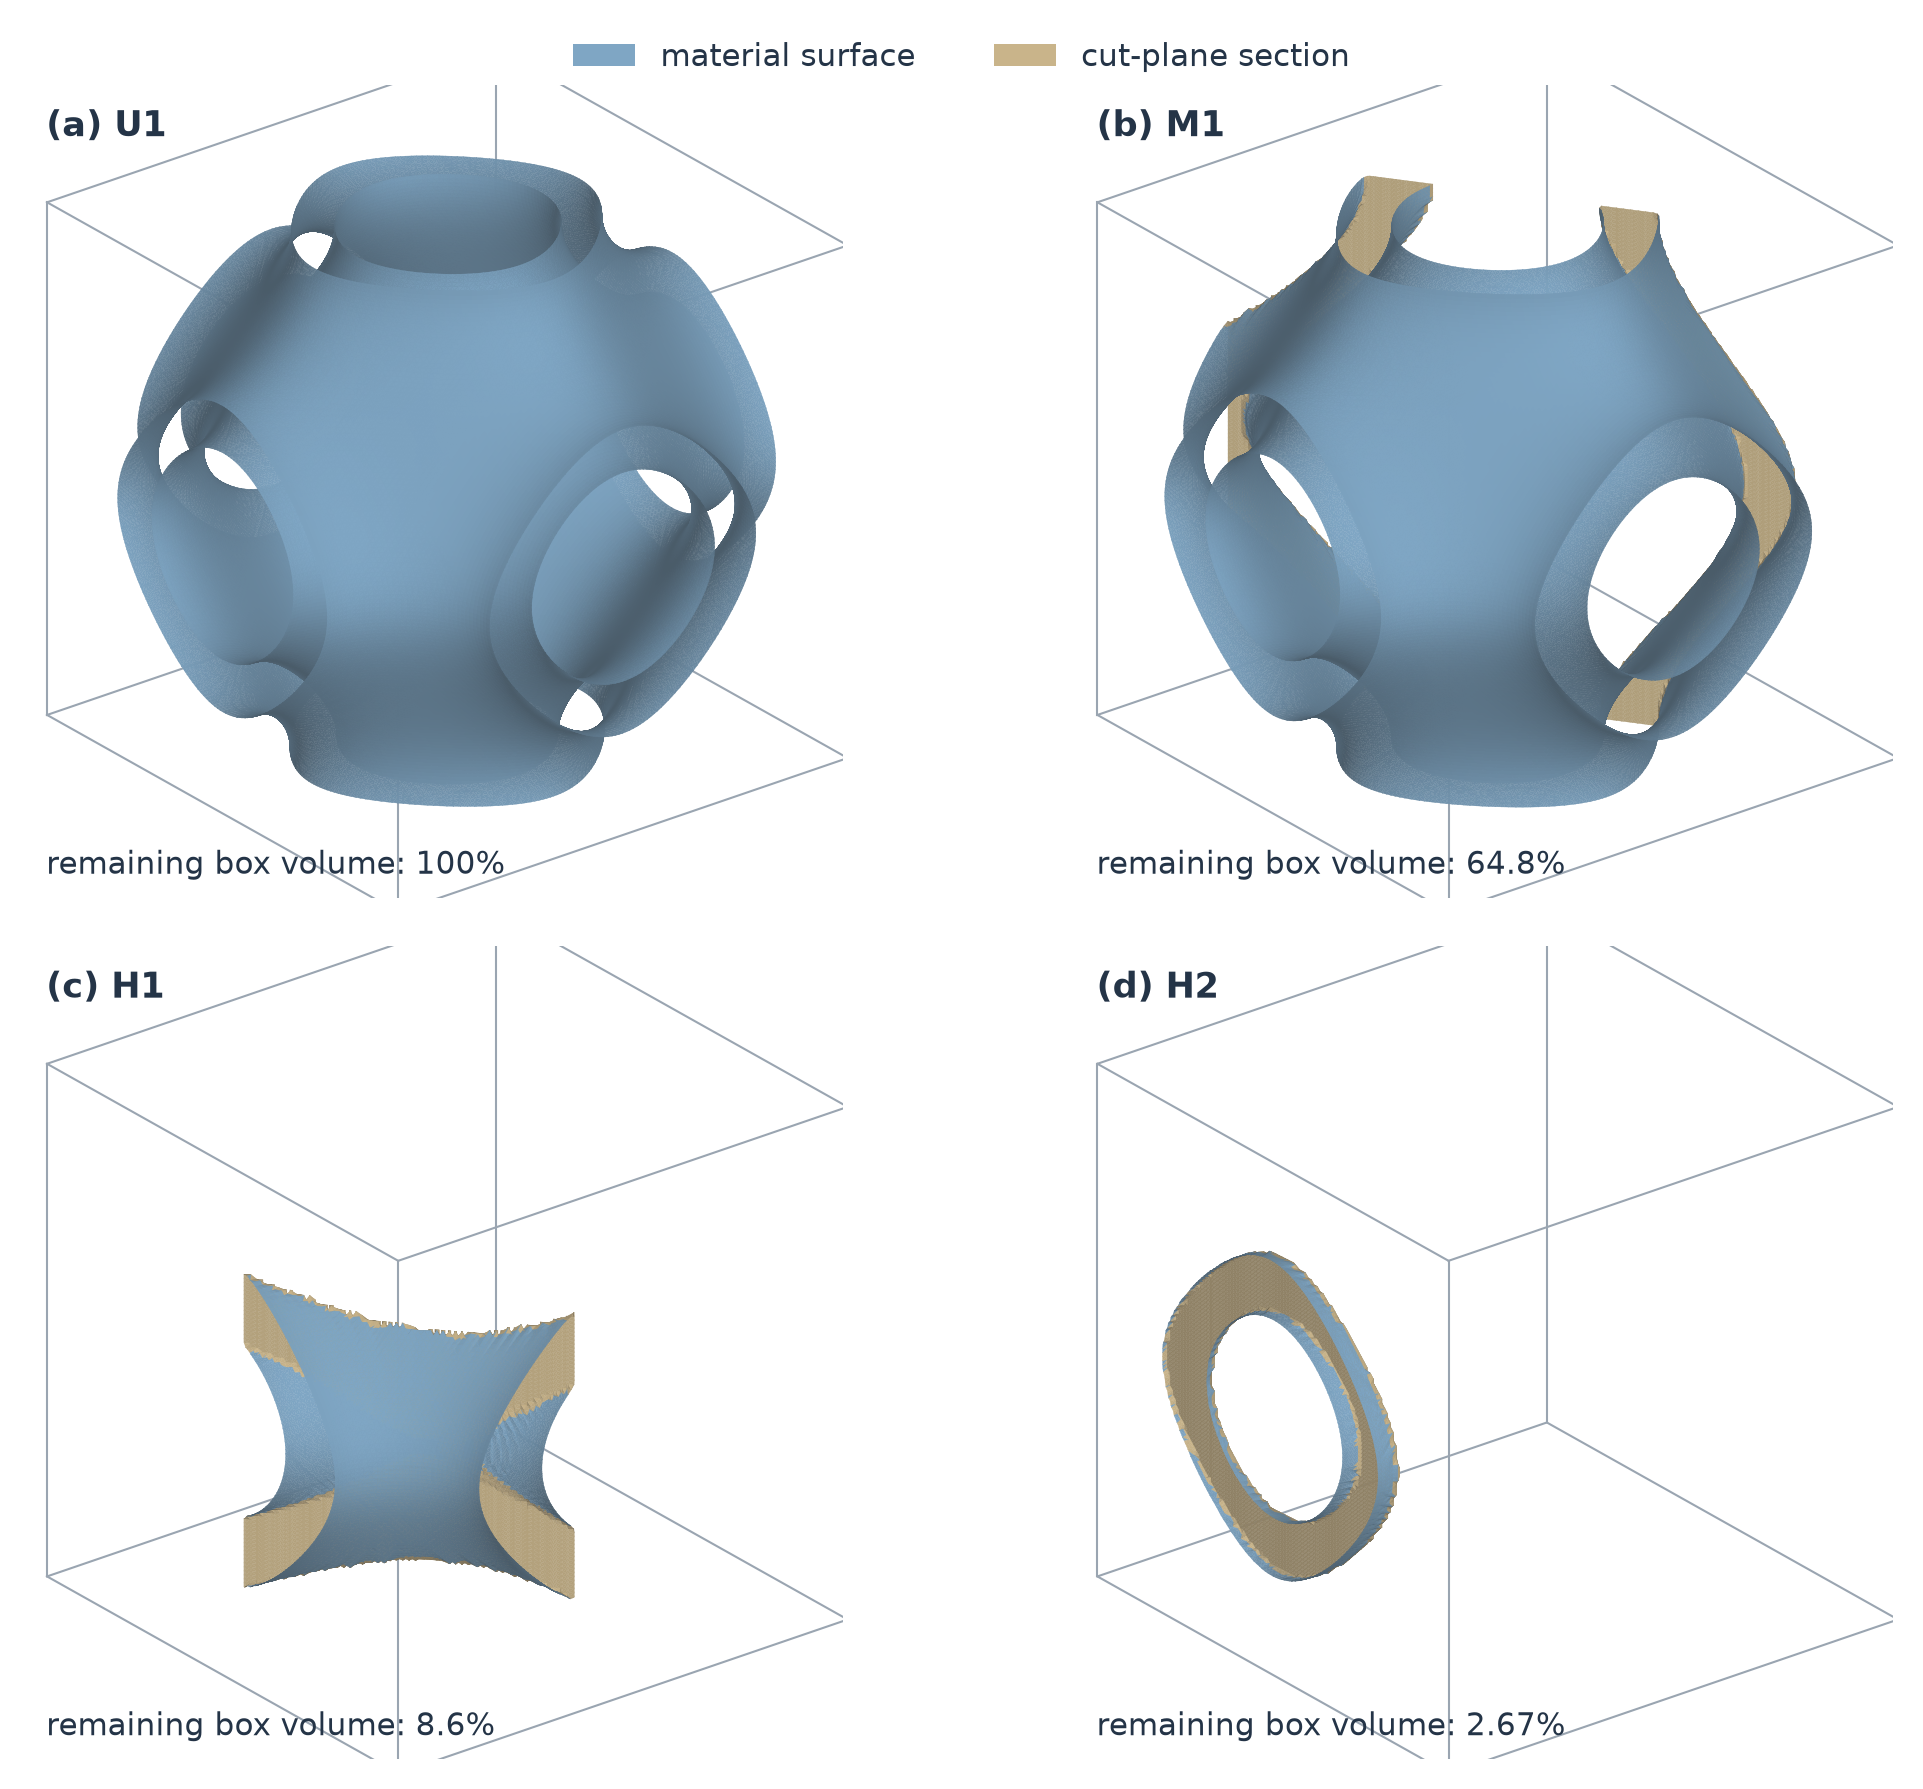
\includegraphics[width=\textwidth]{../figures/F08_geometry.png}
\caption{\textbf{Representative validation geometries.} The same unit-box scale and viewing direction are used for (a) uncut U1, (b) moderately cut M1, and (c,d) heavily cut H1 and H2. Blue denotes the material surface and orange the macro-cut section. Percentages indicate the retained macro-domain volume relative to the unit box, before intersection with the thin-wall material. Surfaces are reconstructed from the trilinear band parameters and cut-plane data in Eq. (1); the visualisation sampling is specified in Supplementary Note S3.}\label{fig:1}
\end{figure}

\subsection{Retained degrees of freedom and equilibrium extension}

The retained coordinates are chosen from the kinematics of cell coupling and the support of the boundary-load functional. For each cell, the set \(P\) contains the active box-face displacement coefficients and all displacement coefficients of active elements carrying a positive-area macro-cut patch. The latter form a cut band: although some of its nodes lie away from the cut plane, their finite element basis functions contribute to displacement and virtual work on that plane. Keeping these coefficients gives the full retained space used throughout prediction and assembly. It includes both intercell and exterior-boundary coordinates; interior equilibrium is approximated within this fixed space.

Let \(I\) denote the remaining internal degrees of freedom, \(p=|P|\), \(i=|I|\), and \(n_a=p+i\). The selectors \(J_P\) and \(J_I\) extract the two sets from the active displacement vector, and \(q=J_Pu\) is the retained displacement. Boundary loads act through \(q\); internal body loads are zero. In the displayed \((P,I)\) ordering, static condensation gives

\[
\begin{aligned}
&K=\begin{bmatrix}K_{PP}&K_{PI}\\K_{IP}&A\end{bmatrix},\qquad
A=K_{II},\qquad
E=\begin{bmatrix}I_p\\-A^{-1}K_{IP}\end{bmatrix},\\
&S=K_{PP}-K_{PI}A^{-1}K_{IP}=E^TKE.
\end{aligned}
\tag{2}
\]

We assume \(K\succeq0\) and \(A\succ0\), so prescribing \(q\) removes every internal zero-energy motion. The equilibrium displacement extension \(u=Eq\) uniquely minimises the discrete energy over \(J_Pu=q\), and \(Sq\) is its work-conjugate retained force. For a connected free substructure, we additionally assume that \(K\) has exactly six rigid-body modes whose restriction to \(P\) has rank six. Figure 2 summarises how the learned extension replaces the interior solve while retaining the same assembly coordinates.

\subsection{Assembly and response measures}

For substructure \(m\), the Boolean assembly map \(B_m\) extracts \(q_m=B_mU\) from the free global retained displacement \(U\). Coincident box-face coordinates are shared; retained cut-band coordinates outside the box faces remain local to their substructure. Fixed homogeneous supports are incorporated into \(B_m\). The reference and approximate assembled systems are

\[
\mathbb K=\sum_mB_m^TS_mB_m,\qquad
\widehat{\mathbb K}=\sum_mB_m^T\widehat S_mB_m,
\qquad
\mathbb K U=f_g,\quad\widehat{\mathbb K}\widehat U=f_g.
\tag{3}
\]

Here \(\widehat S_m\) denotes the approximate condensed stiffness defined in Section 3. Local condensation commutes with assembly because the internal sets are disjoint and all intercell couplings act through retained coordinates. Both systems use the same local stabilised matrices. We assume that the supported reference matrix \(\mathbb K\) is positive definite.

Under a prescribed force \(f_g\), compliance is \(C=f_g^TU\), with \(\widehat C=f_g^T\widehat U\) and relative error \(e_C=|\widehat C/C-1|\). Local operator accuracy is measured by the relative directional energy excess defined in Section 4.1. Thickness sensitivities use the eight-component vector defined in Section 4.3, with relative Euclidean error \(e_s=\|\widetilde{\boldsymbol s}-\boldsymbol s\|_2/\|\boldsymbol s\|_2\). All relative measures use a nonzero reference denominator. Directional means are formed within each geometry before population statistics are computed; Section 6 specifies the geometry and load sets for each comparison.

{\small
\begin{longtable}[]{@{}
  >{\raggedright\arraybackslash}p{(\linewidth - 2\tabcolsep) * \real{0.5000}}
  >{\raggedright\arraybackslash}p{(\linewidth - 2\tabcolsep) * \real{0.5000}}@{}}
\caption{Discretisation and internal-correction settings.}\tabularnewline
\toprule\noalign{}
\begin{minipage}[b]{\linewidth}\raggedright
Quantity
\end{minipage} & \begin{minipage}[b]{\linewidth}\raggedright
Setting
\end{minipage} \\
\midrule\noalign{}
\endfirsthead
\toprule\noalign{}
\begin{minipage}[b]{\linewidth}\raggedright
Quantity
\end{minipage} & \begin{minipage}[b]{\linewidth}\raggedright
Setting
\end{minipage} \\
\midrule\noalign{}
\endhead
\bottomrule\noalign{}
\endlastfoot
Reference geometry & Unit box; P-type implicit band with trilinear corner parameters and an optional planar cut \\
Displacement approximation & Continuous tensor-product \(Q_2\) solid elements on a Cartesian background mesh \\
Background resolution, validation geometries & \(n=32\) elements per axis; \(65\) Q2 node positions per axis \\
Isotropic material, validation geometries & Normalised Young\textquotesingle s modulus \(E_Y=1\), Poisson\textquotesingle s ratio \(\nu=0.3\) \\
Ghost-penalty coefficient, validation geometries & \(\gamma=10^{-4}\) \\
Retained space & Active box-face coefficients and all coefficients of active elements carrying a positive-area macro-cut patch \\
Standard volume integration & \(4^3\) initial subcells; one local refinement of partial subcells; clipped Kuhn tetrahedra with quadrature-rule parameter 4 \\
Smoothing interval & \([b/30,b]\), with \(b=1.05\widehat\lambda_{\max}\) estimated by 40 power iterations \\
Principal interior coarse space & Trilinear vector functions on a \(17^3\)-vertex grid, restricted to the internal degrees of freedom \\
Thickness-difference step & \(h_c=10^{-5}\tau_c\), with fixed active coordinates and ghost contribution \\
Correction of the principal predictor & 8 Chebyshev steps, \(Q_1(17)\) Galerkin solve, 8 Chebyshev steps; same sequence in training and evaluation \\
Arithmetic & Network in single precision (true fp32 convolutions); stiffness actions, smoothing, coarse solve and energies in double precision \\
\end{longtable}}

The mesh, material and stabilisation entries apply to all 80 validation geometries. Length is expressed relative to the unit reference box and the modulus is normalised. Integration and spectral-estimation entries specify the standard implementation. The coarse dimension and smoothing count vary by geometry and correction sequence and are reported with those comparisons. Training populations and the computational benchmark are specified in Tables 2 and 5.

\section{Geometry-conditioned neural displacement extension}

The method combines a geometry-conditioned displacement extension with an internal equilibrium correction. Figure 2 shows how the resulting field defines both the condensed action and the displacement recovered after assembly.

\begin{figure}[!htbp]
\centering
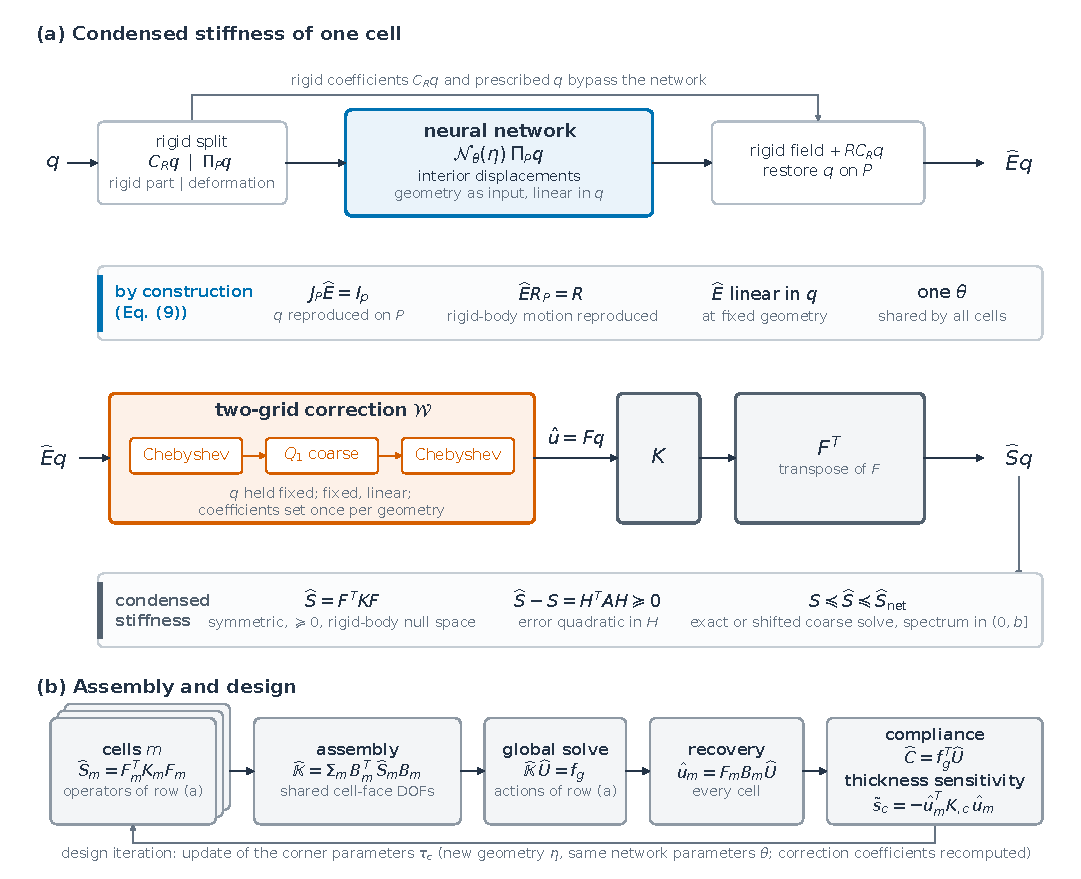
\includegraphics[width=\textwidth]{../figures/F01_method_overview.pdf}
\caption{\textbf{Learned displacement extension, equilibrium correction and variational assembly.} (a) Rigid motion is separated from the retained displacement before the deformation is extended by the network. The rigid field is reconstructed and the prescribed retained values are restored; correction then reduces internal imbalance at fixed retained displacement. (b) Applying the local stiffness and the complete extension transpose gives the work-conjugate retained force. The assembled solution supplies the inputs for local field recovery. The neural extension is detailed in Figure 3; Section 5 defines the internal correction.}\label{fig:2}
\end{figure}

\subsection{Geometry-conditioned multilevel displacement extension}

The learning target is the internal equilibrium map \(q\mapsto E_Iq=-A^{-1}K_{IP}q\). Approximating this map provides both a displacement field and, through its energy, an action of the condensed operator on the complete retained space. Unlike learned shape-function substructures that describe the boundary by a few coordinates \href{https://doi.org/10.1016/j.eml.2023.102041}{Huang et al. (2023)}, \href{https://doi.org/10.1016/j.cma.2026.118955}{Guo et al. (2026a)}, the map is learned on every prescribed retained coordinate. The architecture has two requirements: it must adapt to the distribution of material and support in each cell, and it must respect displacement superposition at a fixed geometry. Figure 3 shows how these requirements lead to a nonlinear geometry branch coupled to a linear, multilevel displacement branch.

Rigid motion is separated before learning. Let \(R\in\mathbb R^{n_a\times6}\) contain three translations and three rotations about a common centre, and let \(R_P=J_PR\). The coefficient extractor \(C_R=(R_P^TR_P)^{-1}R_P^T\) and projector \(\Pi_P=I_p-R_PC_R\) decompose the input into rigid coefficients \(C_Rq\) and retained deformation \(q_d=\Pi_Pq\). The network extends only \(q_d\). This decomposition reserves its approximation capacity for deformation and makes rigid reconstruction independent of training accuracy.

The geometry branch describes where the discrete body carries and transmits stiffness. Element moments resolve the material distribution within each background cell; node features identify retained and cut-band membership, weak support, local stiffness magnitude and position. Encoders form element and node embeddings, which exchange information in two successive rounds. From these embeddings, coefficient heads assign weights to prescribed element and ghost-face incidences, to transfers between latent grids, and to coarse-grid convolutions. The incidence maps and retained-coordinate semantics are deterministic. Geometry conditioning changes their numerical action, with coefficients that remain fixed for all displacement directions on the same geometry.

The displacement branch first lifts the three components of \(q_d\) to 32 channels on retained nodes and sets the internal features to zero, defining \(X^0(q)\). Local interactions then propagate these values through the element and ghost-face neighbourhoods. Each interaction gathers the features on a 27-slot stencil into four weighted heads, mixes the channels within each head, and scatters the result back to the incident nodes. Separate gather and scatter coefficients permit directional coupling across the stencil. With internal and retained masks \(M_I,M_P\) acting on nodal rows, an interaction updates the latent field by

\[
X^{\ell+1}=M_I\left[X^\ell+
 \sum_h\mathcal S_{\ell h}(\eta)
   \big(\mathcal G_{\ell h}(\eta)X^\ell W_{\ell h}\big)\right]
 +M_PX^0(q).
\tag{4}
\]

Here \(\mathcal G_{\ell h}\) and \(\mathcal S_{\ell h}\) are geometry-weighted gather and scatter maps, and \(W_{\ell h}\) mixes channels. The residual form preserves the incoming state, while the final term restores the retained features. Element interactions follow the local \(Q_2\) support, and ghost-face interactions communicate across face neighbourhoods present in the stabilised discretisation. They approximate the displacement response; the mechanical stiffness continues to be defined by \(K\).

Internal equilibrium also couples locations separated by many element neighbourhoods. A U-shaped latent hierarchy supplies this longer-range communication. Four local interaction pairs precede restriction through grids with 65, 33, 17 and 9 positions per axis. At each coarser level, two residual convolutions mix neighbouring latent features. The upward pass applies two further convolutions before prolongation and adds the stored state at the receiving finer level. These additive skips retain local information while the coarse path distributes information across larger distances. All levels carry 32 displacement channels. After returning to the active fine nodes, four local interaction pairs combine the multilevel result with the element and face neighbourhoods, and four additional pairs act on stencils containing weakly supported nodes. A linear 32-to-3 map reconstructs nodal displacement. Appendix G gives the complete order of operations and coefficient definitions.

Every displacement operation is linear: the nonlinear encoders and coefficient bounds act only on geometry. The resulting raw map \(\mathcal N_\theta(\eta)\) therefore obeys superposition for a fixed geometry \(\eta\), despite its nonlinear dependence on that geometry. Adding back the rigid field and restoring the original retained values gives

\[
\widehat E q=J_P^Tq+
J_I^TJ_I\left[RC_Rq+\mathcal N_\theta(\eta)\Pi_Pq\right].
\tag{5}
\]

Consequently, \(J_P\widehat E=I_p\) and \(\widehat ER_P=R\): admissibility and rigid reproduction hold by construction. The latent hierarchy changes how the deformation extension is computed; the mechanical input and output retain their original coordinates. Its learned communication also serves a different purpose from the residual-based equilibrium corrections introduced in Section 5, which act on the reconstructed field using \(K\).

\begin{figure}[!htbp]
\centering
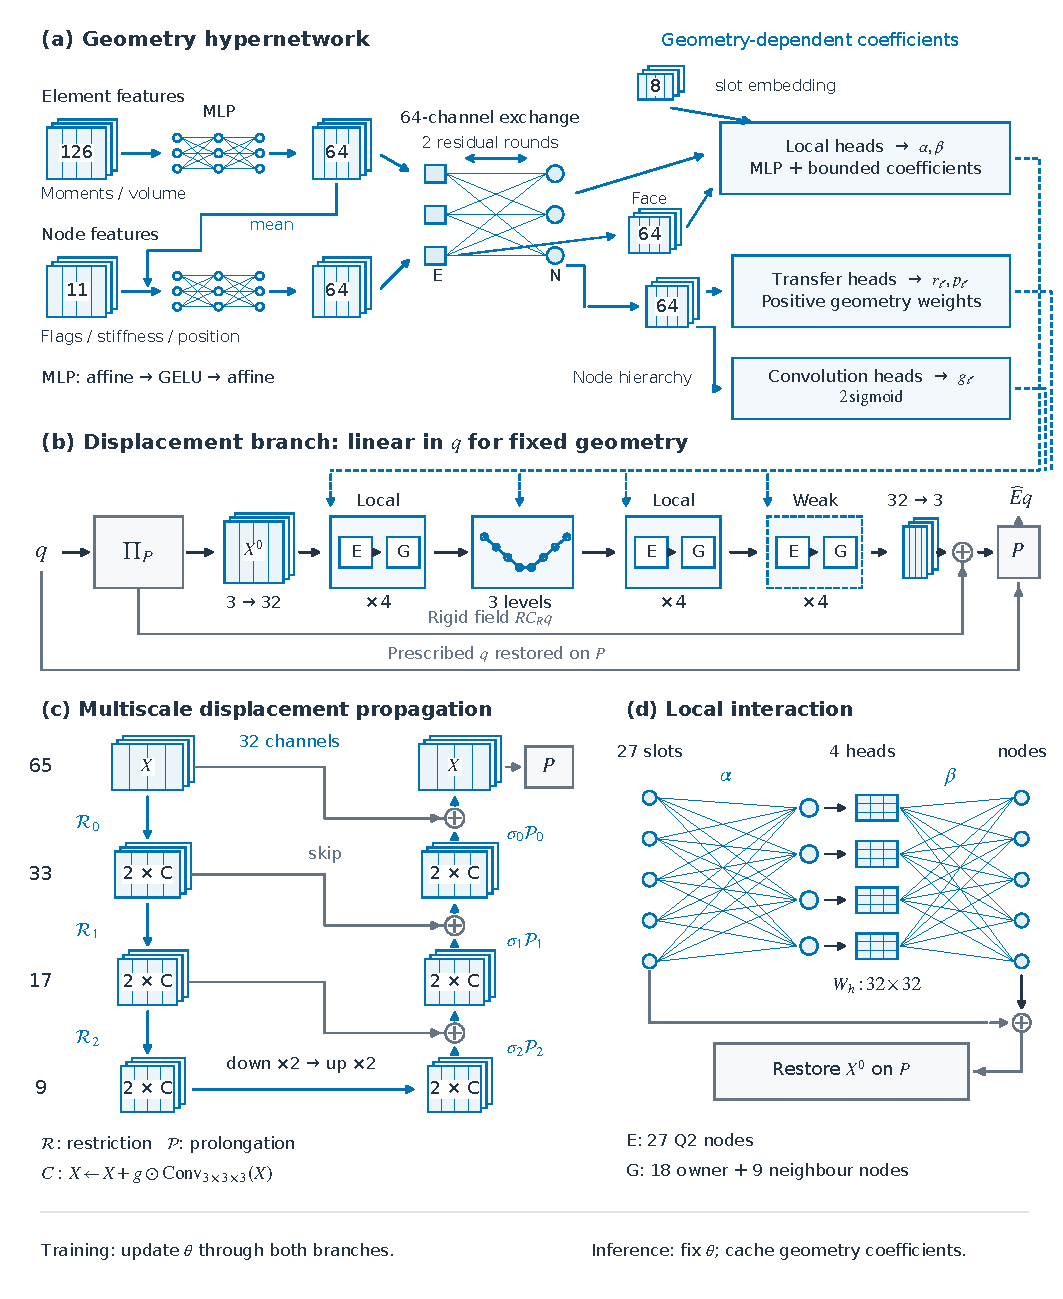
\includegraphics[width=\textwidth]{../figures/F11_network_architecture.pdf}
\caption{\textbf{Geometry-conditioned neural displacement architecture.} (a) Element and node encoders produce 64-channel geometry embeddings, followed by two rounds of residual exchange. Coefficient heads condition the local interactions, grid transfers and convolutions. (b) The displacement branch propagates the nonrigid retained input through four local interaction pairs, the multilevel block, four further local pairs and four pairs on weakly supported stencils. Linear input and output maps connect the three displacement components to 32 latent channels. Deterministic bypasses reconstruct rigid motion and restore the original retained values. (c) Restriction and prolongation connect grids with 65, 33, 17 and 9 background positions per axis; actual active node counts depend on geometry. Each coarse level has two residual convolutions on each pass, and upward transfers combine with additive skips. (d) A local interaction uses geometry-weighted gathering, four channel-mixing heads and scattering, followed by residual addition and retained-value restoration. E and G denote element and ghost-face interactions. Blue dashed arrows carry geometry-dependent coefficients; solid arrows carry features or displacement states. Channel-mixing matrices and convolution kernels are shared trainable parameters. For fixed geometry, the complete displacement path is linear. Training updates parameters through both branches; inference reuses the geometry coefficients.}\label{fig:3}
\end{figure}

\subsection{Variational condensed stiffness}

The learned field becomes a mechanical operator by evaluating its energy with the original local stiffness. Let \(\mathcal W\) be a fixed linear internal correction that preserves retained values, with the identity corresponding to no correction. For each geometry, the correction schedule and its coefficients are fixed independently of the displacement query. The final extension and its condensed stiffness are

\[
F=\mathcal W\widehat E,\qquad
\widehat S=F^TKF,\qquad
\widehat{\mathcal U}(q)=\tfrac12q^T\widehat S q,\qquad
\widehat f_P=\widehat S q.
\tag{6}
\]

Thus a single displacement representation determines the energy and retained force. For a virtual retained displacement \(\delta q\), the corresponding full virtual field is \(F\delta q\), and \(\delta\widehat{\mathcal U}=(F\delta q)^TKFq=\delta q^TF^TKFq\). Applying the condensed operator therefore requires the transpose of the complete extension after the stiffness action. This includes the rigid reconstruction, retained-value restoration and any internal corrections. With \(F_I=J_IF\), its block form is

\[
\widehat S q=(KFq)_P+F_I^T(KFq)_I.
\tag{7}
\]

The second term transfers the work of the internal residual to the retained coordinates. It vanishes for an equilibrated field; otherwise it is needed for the returned force to be the derivative of the stated energy. Symmetry and positive semidefiniteness follow from \(K=K^T\succeq0\), without requiring symmetry of the learned gather, scatter or grid-transfer maps. Under the rigid-kernel assumption of Section 2.2 and \(FR_P=R\), the only null modes of \(\widehat S\) are the retained rigid-body modes. Appendix B proves this statement, and Appendix E derives the complete transpose.

This construction also provides a common field representation for subsequent mechanics. After an assembled solve, \(F_mB_m\widehat U\) supplies the local reconstructed displacement for response and sensitivity evaluation. Accuracy is governed by how closely that field satisfies internal equilibrium. Section 4 quantifies its effect on condensed energy and mechanical response, and Section 5 uses the same residual to correct the field while preserving the retained values.

\subsection{Training directions and objective}

Training probes the extension through retained displacement directions that exercise different forms of local deformation and interaction with neighbouring cells. Prescribed polynomial and multiscale displacements supply broad spatial content. Responses to equilibrated nodal loads and consistent tractions, spring-supported responses, and displacements induced by a neighbouring cell supply mechanically generated directions. Rigid components are removed and each retained direction is normalised to \(q_j^TSq_j=1\) using the reference substructure solution. This energy normalisation makes the objective compare approximation quality across directions with different amplitudes and stiffnesses. For a batch of \(B\) directions, the objective is

\[
\mathcal L(\theta)=\frac1B\sum_{j=1}^{B}\log(q_j^T\widehat S q_j)
 +w_s\frac1{|\mathcal J_s|}\sum_{j\in\mathcal J_s}
 \frac{\|\widetilde{\boldsymbol s}_j-\boldsymbol s_j\|_2^2}{\|\boldsymbol s_j\|_2^2},
\tag{8}
\]

The energy term is the mean logarithm of the predicted-to-reference energy ratio. For an admissible extension, the variational identity in Section 4 makes its minimum correspond to the equilibrium field on each sampled direction. The sensitivity term additionally measures the complete eight-corner vectors, so that training accounts for how the reconstructed field weights the local design derivatives. The set \(\mathcal J_s\) contains directions with reference sensitivity labels; this term is omitted when the set is empty, and the reported configurations use \(w_s=1\). Gradients with respect to \(\theta\) pass through the reconstructed field to the geometry encoders, coefficient heads and linear displacement maps. The stiffness, retained-coordinate maps and rigid basis define the mechanical objective deterministically.

The correction of Section 5 can also be placed inside the training loop. The principal predictor evaluates Eq. (8) on the corrected extension \(F=\mathcal W\widehat E\), with \(\mathcal W\) the eight-step smoothing, trilinear coarse solve and eight-step smoothing sequence of Section 5.2. Because \(\mathcal W\) is linear and fixed for a given geometry, the gradient of Eq. (8) passes through the smoothing recurrence and the coarse solve to the network parameters; the network is thereby trained to supply the initial field that the correction completes, rather than a field that must be accurate on its own. The smoothing interval and coarse factorisation depend only on \(K\) and are recomputed per geometry, so training through the correction adds no trainable parameters.

Finite direction banks sample only part of the retained space. Large-energy-ratio directions are therefore sought by a block search on the rigid complement and by a search within the span of stored directions. Adding them focuses subsequent training on observed weaknesses of the extension. Geometry augmentation uses the 48 cube symmetries with consistent transformations of vector components; predicted fields are returned to the original frame for mechanical evaluation. Appendix G specifies the direction classes, sampling weights, normalisation and optimisation settings. Table 2 identifies the model roles, and Table ST12 records the training and weight-selection settings. The fixed-weight correction study in Section 6.5 changes the internal correction while using the same learned extension.

\section{Extension error and mechanical response}

Once the retained coordinates are fixed, the local approximation lies in the interior field associated with each retained displacement. Its mechanical significance follows from the energy carried by the departure from equilibrium. We first relate this departure to condensed stiffness, then examine how assembly and thickness differentiation weight the same field error. These relations provide the basis for the internal correction in Section 5.

\subsection{Variational energy error}

For the specified symmetric stiffness \(K\succeq0\), with \(A=K_{II}\succ0\) and zero internal body loads, \(Eq\) minimises the energy at prescribed \(q\). Any admissible linear extension \(F\), with \(J_PF=J_PE=I_p\), differs from it only internally. Writing \(H=J_I(F-E)\), internal stationarity \(J_IKE=0\) eliminates the cross terms in \(F^TKF\) and gives the discrete Ritz identity

\[
\boxed{\widehat S-S=H^TAH\succeq0.}
\tag{9}
\]

The learned extension therefore adds stiffness in proportion to the energy of its internal error. The absence of a first-order term follows from equilibrium of the reference field. For \(u=Eq\), \(\widehat u=Fq\) and \(d_I=Hq\), the internal residual \(r_I=(K\widehat u)_I\) satisfies \(r_I=Ad_I\). The relative directional energy excess \(\varepsilon(q)=q^T(\widehat S-S)q/(q^TSq)\) can consequently be written as

\[
\varepsilon(q)=\frac{d_I^TAd_I}{q^TSq}
=\frac{r_I^TA^{-1}r_I}{q^TSq}.
\tag{10}
\]

Equation (10) identifies the squared \(A^{-1}\)-norm of the internal residual as the stiffness-error measure. The residual itself is available from the reconstructed field and the known stiffness, so it also supplies a correction without requiring the reference extension. Appendix B gives the corresponding all-direction norm; evaluation over a finite direction bank samples this energy error.

\subsection{Assembled compliance and energy participation}

The local stiffness excess changes both the global retained solution and the fields recovered within each substructure. Consider the exact equilibria of the two supported systems in Eq. (3), with the same local matrices, fixed assembly maps and homogeneous supports, and the same nonzero retained load. The supported reference stiffness is positive definite as assumed in Section 2.3. Writing \(u_m=E_mB_mU\), \(\widehat u_m=F_mB_m\widehat U\) and \(a(v,v)=\sum_m v_m^TK_mv_m\), global equilibrium and local energy orthogonality give

\[
\boxed{C-\widehat C
=a(\widehat u-u,\widehat u-u)
=\|\widehat U-U\|_{\mathbb K}^{2}
+\sum_m\|H_mB_m\widehat U\|_{A_m}^{2}.}
\tag{11}
\]

Compliance underestimation is therefore the total reconstructed error energy. Its two contributions have distinct mechanical origins: the changed retained solution and the internal departure from equilibrium at that solution. Their orthogonality makes the energy partition exact. The additional work associated with incomplete global equilibrium is treated in Section 5.3.

The influence of a local approximation depends on how much energy that substructure carries under the applied load. At the exact assembled traces \(q_m=B_mU\), define \(w_m=q_m^TS_mq_m/C\) and \(\beta=\sum_mw_m\varepsilon_m(q_m)\). Contributions from rigid zero-energy responses are defined as zero, consistently with the exact rigid reproduction imposed in Section 3. The energy fractions \(w_m\) sum to one, and

\[
0\le\frac{C-\widehat C}{C}\le\frac{\beta}{1+\beta}\le\beta.
\tag{12}
\]

The weighted product \(w_m\varepsilon_m\) links local stiffness error to global work. Small participation can attenuate a substructure\textquotesingle s effect on compliance even when its local field remains inaccurate. Consequently, accurate compliance under a particular load does not establish uniform local accuracy. Appendix J.3 derives this load-specific bound and the associated asymptotic expansion.

\subsection{Field-based sensitivity and the complete design derivative}

Thickness sensitivity weights the field through the change in stiffness caused by a material variation. On a differentiable design interval with fixed active and retained coordinates, assembly maps, homogeneous supports and a design-independent load, the exact compliance sensitivity is \(s_c=-u^TK_{,c}u\), where \(K_{,c}=\partial K/\partial\tau_c\); contributions are summed over affected substructures. Internal stationarity gives \(S_{,c}=E^TK_{,c}E\), eliminating the design derivative of the exact extension from the force-controlled compliance derivative \href{https://doi.org/10.1023/a:1011430410075}{Giles \& Pierce (2000)}.

The field-based estimate \(\widetilde s_c=-\widehat u^TK_{,c}\widehat u\) uses the same stiffness derivative with the reconstructed field. At the same retained displacement,

\[
\widetilde s_c-s_c=-2d^TK_{,c}u-d^TK_{,c}d,
\qquad u=Eq,\quad d=Fq-Eq.
\tag{13}
\]

Internal equilibrium sets \((Ku)_I=0\), but generally leaves \((K_{,c}u)_I\ne0\). The linear cross term in Eq. (13) therefore survives the stationarity that removed it from the stiffness error. Its magnitude relative to the quadratic term depends on the derivative-weighted fields: its presence does not imply first-order dominance at finite error, and decreasing energy error need not decrease sensitivity error monotonically. For corner thickening, nonnegative trilinear shape functions generate nested material domains. With fixed basis, material and ghost contribution, exact integration gives \(K_{,c}\succeq0\); even then the cross term can have either sign. Appendix J.4--J.5 gives the corresponding sensitivity bounds and design assumptions.

Assembly introduces a further field change through \(\Delta q=\widehat q-q\). The local discrepancy becomes \((F-E)q+E\Delta q+(F-E)\Delta q\), combining extension error, changed retained displacement and their interaction. The field-only and solution-only replacements in Section 6 isolate the first or second effect; their sensitivity norms are not additive contributions.

The derivative of surrogate compliance also accounts for the design dependence of the approximate extension. For a parameter affecting one substructure, differentiation at fixed retained coordinates gives

\[
\widehat C_{,c}
=-\widehat u^TK_{,c}\widehat u
 -2\widehat q^TF_{,c}^TK\widehat u
=\widetilde s_c-2(F_{I,c}\widehat q)^Tr_I,
\qquad\widehat u=F\widehat q.
\tag{14}
\]

Here \(\widehat q\) is the surrogate\textquotesingle s assembled retained solution and \(r_I=(KF\widehat q)_I\); affected-substructure contributions are summed. The second term couples the extension\textquotesingle s design dependence to its internal imbalance and vanishes for an equilibrated extension. The reported field-based estimates contain only the first term. A uniformly \(C^1\)-small extension error is sufficient for quadratic accuracy of the complete derivative, as shown by Eq. (J.5) in Appendix J.5; energy accuracy alone does not supply that design-derivative control. Appendix H specifies the numerical stiffness derivatives.

The eight-component vector refers to local corner parameters. For shared design variables \(\boldsymbol\tau_g\) enforcing continuity through \(\boldsymbol\tau_m=\boldsymbol\tau_m(\boldsymbol\tau_g)\), the structural gradient is \(\nabla_{\boldsymbol\tau_g} C=\sum_m(\partial\boldsymbol\tau_m/\partial\boldsymbol\tau_g)^T\boldsymbol s_m\) under the fixed load and assembly maps above. The same parameter map acts on the complete derivatives in Eq. (14) for surrogate compliance.

\section{Internal equilibrium correction}

The stiffness-error identity in Eq. (10) and the compliance relation in Eq. (11) suggest correcting the learned field by reducing its internal imbalance while preserving the retained motion. Polynomial relaxation and coarse energy minimisation address different components of that imbalance within the existing assembly space. Their effect on sensitivity remains governed by the derivative-weighted relations in Eqs. (13)--(14).

\subsection{Error spectrum and polynomial relaxation}

The internal spectrum resolves the error into components on which relaxation acts differently. Set \(D=\operatorname{diag}(A)\) and order the generalised eigenvectors by increasing eigenvalue, \(Av_j=\lambda_jDv_j\), with \(v_j^TDv_k=\delta_{jk}\). For \(c_j=v_j^TDd_I\),

\[
d_I^TAd_I=\sum_j\lambda_jc_j^2,\qquad
\chi_\ell(q)=\frac{\sum_{j=1}^{\ell}\lambda_jc_j^2}{d_I^TAd_I}.
\tag{15}
\]

The fraction \(\chi_\ell\) locates the error energy carried by the first \(\ell\) Jacobi-scaled internal modes. The corresponding exact-field fraction uses its own denominator \(u_I^TAu_I\). These spectra describe relaxation at fixed retained displacement, whereas Eq. (B.8) compares the full error with the loaded response. Polynomial relaxation attenuates the modal coefficients according to their eigenvalues, and a coarse space is chosen to address slowly relaxed interior error.

For each retained input, the learned field provides an initial approximation to \(Au_I=-K_{IP}q\). We apply Jacobi-preconditioned Chebyshev semi-iteration with \(q\) fixed. A prescribed iteration count and geometry-dependent coefficients make the corrected extension linear in displacement, as required for one condensed stiffness operator. Polynomial relaxation supplies a parallelisable component of multigrid methods \href{https://doi.org/10.1016/s0021-9991(03)00194-3}{Adams et al. (2003)}; pairing it with a learned initial field exploits their complementary error-reduction properties \href{https://doi.org/10.1038/s42256-024-00910-x}{Zhang et al. (2024)}.

For a degree-\(k\) error polynomial, the update is \(P_kd_I\), where \(P_k=p_k(D^{-1}A)\). Each coefficient in Eq. (15) is multiplied by \(p_k(\lambda_j)\), connecting the polynomial directly to the error-energy distribution. The Chebyshev polynomial targets \([a,b]\), \(0<a<b\), and is nonexpansive in the \(A\)-energy norm if the actual positive spectrum of \(D^{-1/2}AD^{-1/2}\) lies in \((0,b]\). Modes below \(a\) can decay slowly, providing the reason for a complementary coarse update. The correction sequences use \(a=b/30\), with \(b\) from a power estimate increased by 5\%; on all 80 validation geometries this endpoint exceeds the converged largest eigenvalue by 2.1--5.0\%. Appendix D gives the polynomial, recurrence, interval estimator, this verification and the contraction bound.

\subsection{Interior coarse correction}

A coarse update removes the part of the remaining error accessible to a prescribed interior space. Let \(V\in\mathbb R^{i\times n_c}\) have full column rank, \(A_c=V^TAV\), and \(b_r=V^Tr_I\). Minimising the energy over \(u_I+\operatorname{range}V\) gives

\[
u_I^{\rm c}=u_I-VA_c^{-1}b_r,\qquad
d_I^{\rm c}=(I_i-VA_c^{-1}V^TA)d_I,\qquad
\|d_I\|_A^2-\|d_I^{\rm c}\|_A^2=b_r^TA_c^{-1}b_r.
\tag{16}
\]

The Galerkin solve enforces equilibrium against the coarse variations, and the last equality measures the energy removed by that projection \href{https://doi.org/10.1137/1034116}{Xu (1992)}. The principal basis consists of trilinear vector functions on a \(17^3\)-vertex grid restricted to internal fine-grid coordinates. Other resolutions and quadratic interpolation provide the comparisons in Section 6.5. All preserve the full retained space. Appendix F specifies the generating families, basis construction and numerical coarse solves.

Placing the coarse update between two \(k\)-step smoothing stages combines these corrections. With \(C_V=I_i-VA_c^{-1}V^TA\) and \(H_0=J_I(\widehat E-E)\), the resulting error is

\[
H_{\rm tg}=P_kC_VP_kH_0,\qquad
\widehat S_{\rm tg}-S=H_{\rm tg}^TAH_{\rm tg}.
\tag{17}
\]

For the exact Galerkin update and \(\|P_k\|_A\le1\), \(S\preceq\widehat S_{\rm tg}\preceq\widehat S_0\). The combined correction therefore removes variational stiffness excess while preserving the condensation target. This ordering also moves exact assembled compliance toward the reference through Eq. (11), although it does not order the sensitivity error in Eq. (13). Appendices D and F state how the polynomial and coarse-solve conditions relate to the actual correction matrices.

\subsection{Energy-consistent operator application}

The corrected field and returned force must derive from the same energy. Geometry-dependent coefficients, maps, smoothing interval and coarse factorisation are prepared once and reused across retained inputs.

\textbf{Algorithm 1. Corrected condensed stiffness action.}

\begin{enumerate}
\def\labelenumi{\arabic{enumi}.}
\tightlist
\item
  Extend \(q\) with \(\widehat E\) and apply the prescribed pre-smoothing, coarse and post-smoothing sequence at fixed retained values to obtain \(u=Fq\).
\item
  Form \(y=Ku\) and return \(F^Ty\): transpose the complete correction in reverse order, followed by the transpose learned extension.
\item
  Assemble these actions through Eq. (3); after the global solve, recover \(F_mB_m\widehat U\) for field and sensitivity evaluation.
\end{enumerate}

Each forward cycle uses \(2k\) smoothing steps and one coarse solve, with the corresponding reverse operations in the transpose. Appendices E--F give the actions, factorisation and arithmetic details.

At the assembled level, the energy relation also separates approximation error from incomplete equilibrium. For an approximate solution \(\bar U\), define the recomputed residual \(\rho=f_g-\widehat{\mathbb K}\bar U\) using the stated variational operator and the recovered fields \(\bar u_m=F_mB_m\bar U\). Then

\[
C-f_g^T\bar U=a(\bar u-u,\bar u-u)+\bar U^T\rho.
\tag{18}
\]

The signed residual work determines how incomplete solution affects the compliance comparison. Its sign and magnitude depend on the residual and displacement together. Appendix J.6 gives the residual-corrected functional and the additional consistency term required when the numerical action differs from the energy operator.

\section{Numerical examples}

The examples follow the error of a learned local extension into the quantities required for assembled analysis. Population results identify its dependence on geometry and loading; fixed-weight comparisons then establish how much the local error can be reduced by correcting interior equilibrium. The assembled responses examine the distinct accuracy requirements of global compliance and local thickness sensitivity. These are the principal comparisons, with retained-space restriction and computational cost providing complementary perspectives. Response errors are measured against equilibrium of the discrete elastic problem in Section 2.

\subsection{Geometries, predictors and loading conditions}

The 80 validation geometries span uncut, lightly cut, moderately cut and heavily cut cells, with 20 geometries in each stratum. They use the material parameters and background discretisation in Table 1 and comprise 20 uniform, 30 affine and 30 mixed trilinear thickness fields. Their corner parameters range from 0.1762 to 0.6983. Canonical cut normals are \((\cos\vartheta,\sin\vartheta,0)\), with \(0<\vartheta<\pi/4\). Cut severity refers to the retained macro-box volume before intersection with the TPMS material: heavy cuts retain less than one third, moderate cuts between one and two thirds, and light cuts more than two thirds. Table ST11 gives the parameter domain and stratum-specific ranges. U, M and H identify the selected uncut, moderately cut and heavily cut cells used for detailed comparisons.

The predictors in Table 2 separate the contribution of the network, of the correction and of training through the correction. The principal predictor A3 continues B on the larger training population with the complete correction of Section 5.2 inside the training loop (Section 3.3) and applies the same correction when evaluated. B supplies the fixed network for the local correction examples; B+W applies A3\textquotesingle s correction to B\textquotesingle s unchanged weights, isolating the effect of training through the correction. C continues B without correction. S8 continues B with eight smoothing steps at evaluation; only part of its training steps passed through the smoothing stage, so S8 is used as a comparison predictor and not interpreted as a trained smoothing variant. A2b continues B with eight smoothing steps included in every training step and no coarse solve. P0 provides a reference trained on a smaller population. The historical computational examples use a separate uncorrected predictor D.

{\small
\begin{longtable}[]{@{}
  >{\raggedright\arraybackslash}p{(\linewidth - 8\tabcolsep) * \real{0.1875}}
  >{\raggedright\arraybackslash}p{(\linewidth - 8\tabcolsep) * \real{0.1875}}
  >{\raggedleft\arraybackslash}p{(\linewidth - 8\tabcolsep) * \real{0.2500}}
  >{\raggedright\arraybackslash}p{(\linewidth - 8\tabcolsep) * \real{0.1875}}
  >{\raggedright\arraybackslash}p{(\linewidth - 8\tabcolsep) * \real{0.1875}}@{}}
\caption{Learned predictors and their roles in the numerical comparisons.}\tabularnewline
\toprule\noalign{}
\begin{minipage}[b]{\linewidth}\raggedright
Predictor
\end{minipage} & \begin{minipage}[b]{\linewidth}\raggedright
Role in the comparison
\end{minipage} & \begin{minipage}[b]{\linewidth}\raggedleft
Training geometries
\end{minipage} & \begin{minipage}[b]{\linewidth}\raggedright
Correction in training
\end{minipage} & \begin{minipage}[b]{\linewidth}\raggedright
Correction at evaluation
\end{minipage} \\
\midrule\noalign{}
\endfirsthead
\toprule\noalign{}
\begin{minipage}[b]{\linewidth}\raggedright
Predictor
\end{minipage} & \begin{minipage}[b]{\linewidth}\raggedright
Role in the comparison
\end{minipage} & \begin{minipage}[b]{\linewidth}\raggedleft
Training geometries
\end{minipage} & \begin{minipage}[b]{\linewidth}\raggedright
Correction in training
\end{minipage} & \begin{minipage}[b]{\linewidth}\raggedright
Correction at evaluation
\end{minipage} \\
\midrule\noalign{}
\endhead
\bottomrule\noalign{}
\endlastfoot
\textbf{A3} & \textbf{Principal predictor} & 591 & 8 / \(Q_1(17)\) / 8 & 8 / \(Q_1(17)\) / 8 \\
B+W & B\textquotesingle s weights with A3\textquotesingle s correction, untrained & 305 & None & 8 / \(Q_1(17)\) / 8 \\
A2b & Smoothing-only training & 591 & 8 steps & 8 steps \\
S8 & Comparison predictor & 591 & Partial (see text) & 8 steps \\
C & Uncorrected continuation & 591 & None & None \\
B & Fixed weights for the local correction study & 305 & None & None \\
P0 & Reference with a smaller training population & 148 & None & None \\
\end{longtable}}

All predictors share the architecture of Section 3 (603,464 trainable parameters) and the same validation set. A3, A2b, C and S8 continue B for 15,000 steps; B was trained for 40,000 steps with weights selected at step 30,000. A3\textquotesingle s continuation took 2.7 h on one NVIDIA GeForce RTX 5090 (peak device memory 29.6 GB). Table ST01 specifies direction-class coverage, and Table ST12 gives training schedules, weight selection and evaluation orientations.

Two properties of the evaluation data are relevant to the comparisons. First, the weights of the continued predictors were selected on a validation list whose first 40 geometries include 20 of the 80 reported validation geometries (6 uncut, 14 cut); selection compared two checkpoints per predictor. Population statistics are therefore also reported for the 60 geometries that did not enter selection. Second, the cells used in the assembly examples served repeatedly as development cases during method development, so the assembly results characterise these configurations rather than an independent test sample. All geometries carry a single planar cut with normal \((\cos\vartheta,\sin\vartheta,0)\); multiple cuts per cell and curved boundaries are outside the present study.

Population statistics first average directional energy excess within each geometry and loading class, then give equal weight to the available geometries. The five basic classes, consistent tractions and single-face consistent tractions cover all 80 geometries; stiffness-scaled supports and neighbour-induced displacements cover 75 (Figure 5 and Table ST01). The population maximum is consequently the largest geometry-level direction mean. This aggregation separates variation across geometries from variation among directions within one cell.

The assembly examples join a learned target to an exact neighbouring cell, with continuous thickness parameters across their common interface. Figure 4 defines the two configurations, supports and load locations. The assembly accuracy solves use preconditioned conjugate gradients with the exact assembled reference factor as preconditioner. Each configuration has six face loads: the three Cartesian traction directions applied separately to the target and neighbour faces. Compliance and each cell\textquotesingle s eight-parameter sensitivity vector are compared with their exact counterparts. For sensitivity evaluation, the assembled nodal load is held fixed at its base-design value. We use 3\% as a common accuracy reference, taking maxima over the six loads and, for sensitivity, both cells. Three additional tractions on a target cut face are considered separately. Configurations x and y identify the adjoining side.

\begin{figure}[!htbp]
\centering
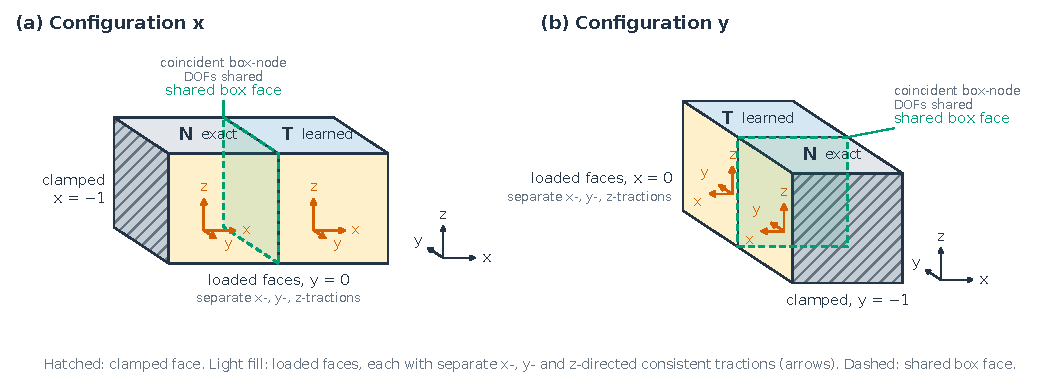
\includegraphics[width=\textwidth]{../figures/F09_assembly_loads.pdf}
\caption{\textbf{Supports and loading of the two-cell examples.} Box envelopes define the coordinate convention. (a) Configuration x: the neighbour is translated by \((-1,0,0)\), the face \(x=-1\) is clamped, and face tractions act at \(y=0\). (b) Configuration y: the translation is \((0,-1,0)\), the face \(y=-1\) is clamped, and tractions act at \(x=0\). Each target (T) and neighbour (N) face carries separate x-, y- and z-directed consistent-traction loads. Coincident box-node coordinates are shared across the interface; non-box cut-band coordinates remain local. Cut targets also receive three macro-cut tractions, analysed separately from the six face loads.}\label{fig:4}
\end{figure}

\subsection{Verification of the discrete reference and of the corrected operator}

All errors in this section are measured against equilibrium of the stabilised discrete problem of Section 2, so two properties must be established first: that this reference approximates the elastic response of the thin-walled cells, and that the implemented operator possesses the structure assumed in Sections 3--5.

For the reference, single cells are clamped on one box face and loaded by a unit consistent traction on another face carrying material, in each Cartesian direction, at background resolutions \(n=24\) to 48 (Figure S06). On the moderately cut M1, the compliance at \(n=32\) differs from that at \(n=48\) by at most 0.057\% over the three load directions, and by 0.21\% at \(n=24\). On the heavily cut H1, whose retained part carries no material on its \(z\)-faces and is therefore clamped on \(x=0\) and loaded on \(y=0\), the corresponding differences from \(n=48\) are at most 0.99\% at \(n=32\) and 2.1\% at \(n=24\), the largest for the in-plane load that bends the remaining wall segments. For heavily cut cells the discretisation error of the reference at \(n=32\) is thus of order one percent, an order of magnitude above the energy errors of the corrected predictor reported below; the comparisons in this section measure the approximation of the discrete operator, not of the continuum. The ghost-penalty contribution to the energy of these loaded fields is \(5\times10^{-5}\) of the total at \(n=32\) and decreases with refinement (from \(1.5\times10^{-4}\) at \(n=24\) to \(1.5\times10^{-5}\) at \(n=48\) on M1). The moderately cut M2 and the uncut U1 behave like M1: at \(n=32\) their compliances differ from the finest level by at most 0.057\% (M2, \(n=48\)) and 0.025\% (U1, \(n=40\)). The eight-corner sensitivities converge at the same rate; at \(n=32\) they differ from the finest level by at most 0.11\% for M1, M2 and U1 and by 0.97\% for H1. Varying the penalty coefficient between \(10^{-5}\) and \(10^{-3}\) changes the compliance by at most 0.053\% and the sensitivities by at most 0.12\% in the four cells, the penalty energy rising to about \(4\times10^{-4}\) of the total at \(\gamma=10^{-3}\). Refining the volume integration (a second level of subcell refinement, or \(6^3\) initial subcells) changes the compliance and the sensitivities by at most 0.010\%. The central-difference stiffness derivative used for the reference sensitivities agrees with central differences of the re-solved compliance to better than \(10^{-6}\) (relative) and changes by less than \(10^{-7}\) when the step is varied between \(10^{-6}\tau_c\) and \(10^{-3}\tau_c\).

For the operator, the deployed implementation evaluates the network in single precision and the stiffness actions, smoothing and coarse solve in double precision. On U2, M1, M2, H1 and H2, the bilinear form \(q_i^T\widehat Sq_j\) is symmetric to a relative \(3\times10^{-8}\), the returned work \(q^T\widehat Sq\) agrees with the energy of the recovered field \(q^TF^TKFq\) to \(2\times10^{-8}\), and the deployed operator reproduces the training-time field to \(1.1\times10^{-7}\). The rigid-body energy \(r^T\widehat Sr\) of normalised rigid modes is at most \(2\times10^{-11}\) of a typical deformation energy. The Chebyshev interval requires \(b\ge\lambda_{\max}(D^{-1}A)\) for the energy contraction of Section 5.1; the power-iteration estimate \(b\) exceeds the Lanczos value of \(\lambda_{\max}\) by 3.9--4.3\% in all five cells, whereas the guaranteed Gershgorin bound exceeds it by factors of 11 to 20 and would slow the smoothing accordingly. These margins refer to the interval estimates of the deployed runs; the 80-geometry check in Appendix D uses its own power-iteration start. The contraction condition is therefore verified per cell rather than guaranteed a priori. Table ST19 and Supplementary Note S5 give the per-cell values.

\subsection{Dependence on geometry and loading}

Consistent tractions are the principal loading class. They represent the surface loads and neighbour tractions of an assembled structure, and the energy of their exact fields resides almost entirely in the bulk material: the ghost-penalty contribution is below 0.05\% of the exact field energy in all cells examined in Section 6.4. Equal nodal forces on the retained coordinates, by contrast, also load weakly supported nodes of small cut elements, and 49--81\% of the corresponding exact field energy resides in the ghost-penalty term. The nodal-force class is therefore retained as a stress test of the stabilised discrete problem, not as the measure of mechanical accuracy.

The principal predictor removes most of the geometric dependence of the uncorrected extension (Figure 5). Under consistent tractions, A3\textquotesingle s mean directional energy excess is 0.016\%, 0.079\%, 0.091\% and 0.109\% across the uncut, lightly, moderately and heavily cut strata of all 80 geometries (0.074\% overall, largest geometry mean 0.65\%), compared with 1.03\%, 5.33\%, 7.82\% and 11.2\% for the uncorrected continuation C (6.33\% overall, largest geometry mean 42\%). The same holds for the loading classes that probe assembly: neighbour-induced retained displacements give a mean of 0.060\% (largest geometry mean 0.38\%) and spring-supported faces 0.057\% (0.47\%). On the nodal-force stress test, B\textquotesingle s mean increases from 0.908\% in uncut cells to 11.3\% in heavily cut cells, with a largest geometry mean of 70.1\%, whereas A3\textquotesingle s stratum means lie between 0.0135\% and 0.0897\% and its largest geometry mean is 0.325\%. Restricting the statistics to the 60 geometries that did not enter weight selection leaves A3\textquotesingle s means essentially unchanged: 0.077\% against 0.074\% under consistent tractions and 0.0591\% against 0.0579\% under nodal forces.

The intermediate predictors locate this improvement. Under consistent tractions, B\textquotesingle s mean is 6.89\% (largest geometry mean 48.6\%), and continuing it without correction (C) changes this only marginally, to 6.33\%. Evaluating with eight smoothing steps (S8) reduces the mean to 1.51\% and training through the smoothing (A2b) to 1.28\%, still with largest geometry means of 9.2\% and 7.8\%; the complete correction trained end to end (A3) reaches 0.074\%. Applying the same correction to B\textquotesingle s unchanged weights (B+W) already gives 0.0965\% (largest geometry mean 0.91\%; strata 0.029\%, 0.096\%, 0.105\% and 0.156\%), so most of the population improvement comes from the correction itself, and training through it reduces the remaining mean by a further factor of 1.3 and the heavy-stratum mean by 1.4. The fixed-weight examples in Section 6.5 separate the contribution of the correction from that of the network weights.

Orientation supplies another source of variation. On the 20 geometries of an earlier evaluation in both orientations, the tested nonidentity cube transformation changes B\textquotesingle s consistent-traction mean from 6.62\% to 7.49\% (Table ST01c). Thus the transformed examples expose differences that are hidden by evaluation in a single orientation. The distributions in Table ST01 and Figure S01 motivate examining both the magnitude and the internal structure of the extension error.

\begin{figure}[!htbp]
\centering
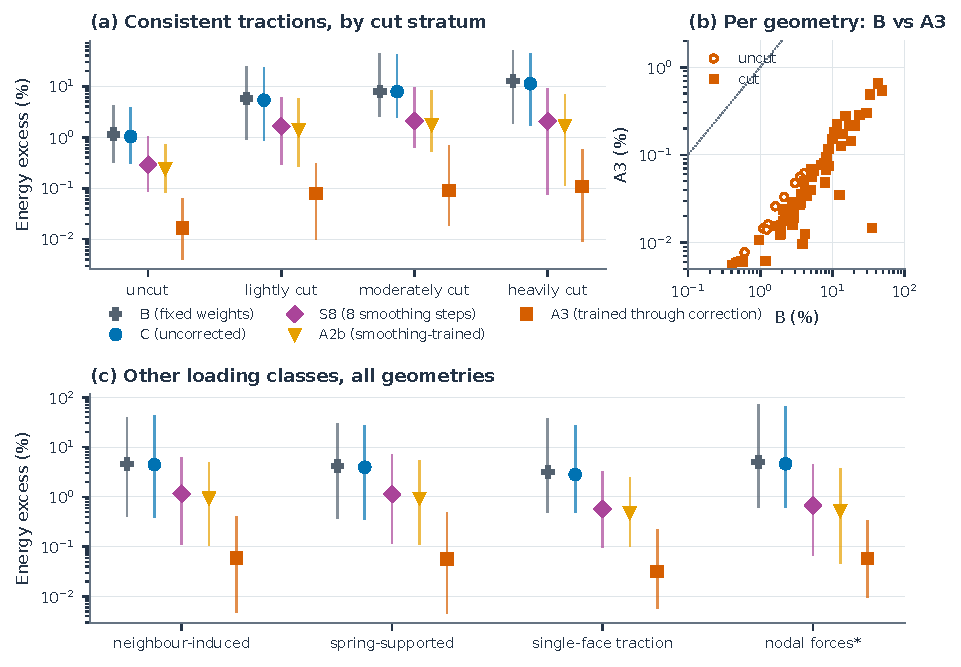
\includegraphics[width=\textwidth]{../figures/F02_validation_A3.pdf}
\caption{\textbf{Directional energy error of the learned substructures on 80 unseen geometries.} Each observation is a geometry\textquotesingle s mean directional energy excess \(q^T(\widehat S-S)q/(q^TSq)\) over the validation directions of a loading class. (a) Consistent tractions, 20 geometries per cut stratum: markers give the mean over geometries and bars the range from the 10th percentile to the maximum. (b) Geometry means of B and of the principal predictor A3 under consistent tractions; the dotted line denotes equality. (c) Neighbour-induced retained displacements, spring-supported faces, single-face consistent tractions and equal nodal forces, all available geometries (75 for the first two classes, 80 for the others); the nodal-force class is a stress test whose exact energy resides largely in the ghost penalty. Predictors as in Table 2.}\label{fig:5}
\end{figure}

\subsection{Components of the extension error}

To relate the geometric variation to interior equilibrium, we examine where B\textquotesingle s field error lies in the Jacobi-scaled internal spectrum (Figure 6). Under consistent tractions on M1, the lowest 200 modes contain 24.5\% of the error energy and 4.87\% of the exact-field energy. These modes have eigenvalues from \(5.74\times10^{-4}\) to \(1.13\times10^{-2}\), all below the lower endpoint \(a=0.173\) of the smoothing interval. In H2, the corresponding eigenvalue range is \(2.13\times10^{-2}\) to \(0.416\), and 66 of the 200 modes lie below \(a=0.138\). The error thus occupies different parts of the spectrum targeted by relaxation. These low-mode locations are consistent with the different smoothing rates examined in Section 6.5 and motivate an additional correction for slowly relaxed components.

The spectral distribution also depends on loading within the same cell. For U1, the lowest 200 modes contain 24.0\% of the error energy and 8.50\% of the exact-field energy under consistent tractions, compared with 5.04\% and 7.98\% under nodal forces. This reversal at fixed geometry shows why the error spectrum must be assessed for the response directions of interest. Table ST02b gives the eigenvalue endpoints and their relation to the smoothing intervals. These modes describe the internal problem at prescribed retained displacement.

\begin{figure}[!htbp]
\centering
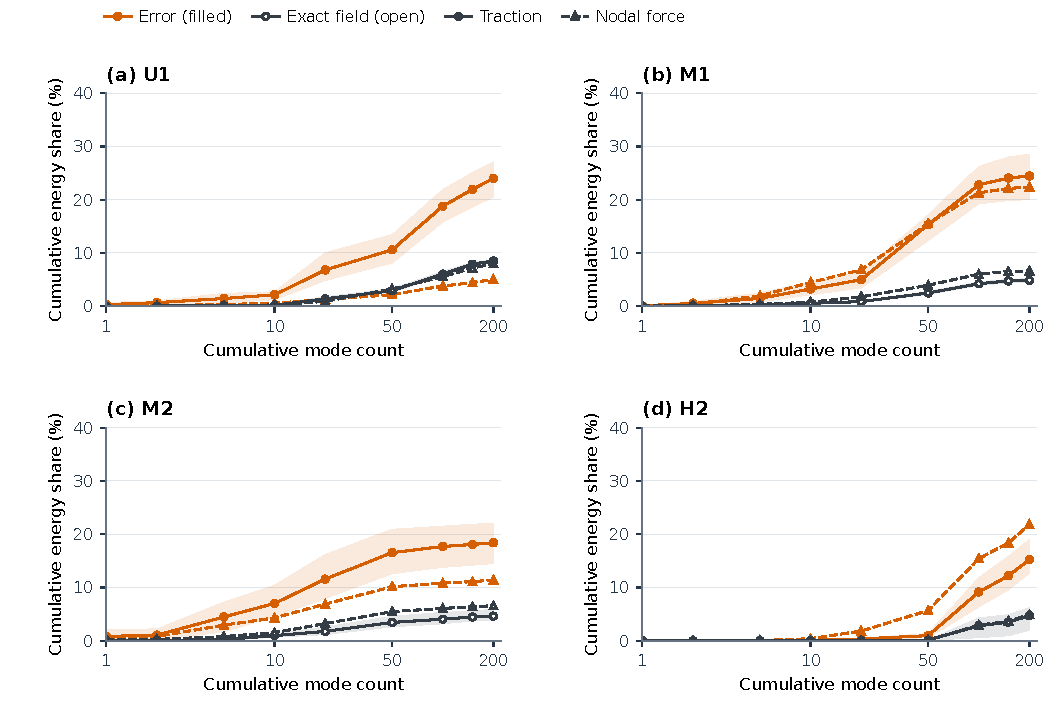
\includegraphics[width=\textwidth]{../figures/F03_spectrum.pdf}
\caption{\textbf{Spectral distribution of the uncorrected extension error.} Panels show U1, M1, M2 and H2 for predictor B. Modes solve \(Av=\lambda Dv\), with \(A=K_{II}\) and \(D=\operatorname{diag}(A)\), and are ordered by increasing eigenvalue. Filled orange markers represent the extension error and open grey markers the exact internal field. Solid circles correspond to consistent tractions and dashed triangles to nodal forces. Curves are directional means; bands give the 10th--90th directional percentiles under consistent tractions. Each cumulative fraction uses the total internal energy of its own field or error as denominator.}\label{fig:6}
\end{figure}

Where in the cell the error resides is shown in Figure 7 for M1 under one consistent-traction direction. The exact field distributes its energy over the thin walls, with 8\% of it in the layer of elements within two element widths of the cut plane, a layer that contains 13\% of the elements. B\textquotesingle s error energy is concentrated in the same layer: across four directions, 39--43\% of it lies there, adjacent to the retained cut-band coordinates whose values the extension must propagate into the interior. The corrected field reduces the element error energies by two to three orders of magnitude throughout the cell and halves the share of the cut-adjacent layer to 19--22\%.

\begin{figure}[!htbp]
\centering
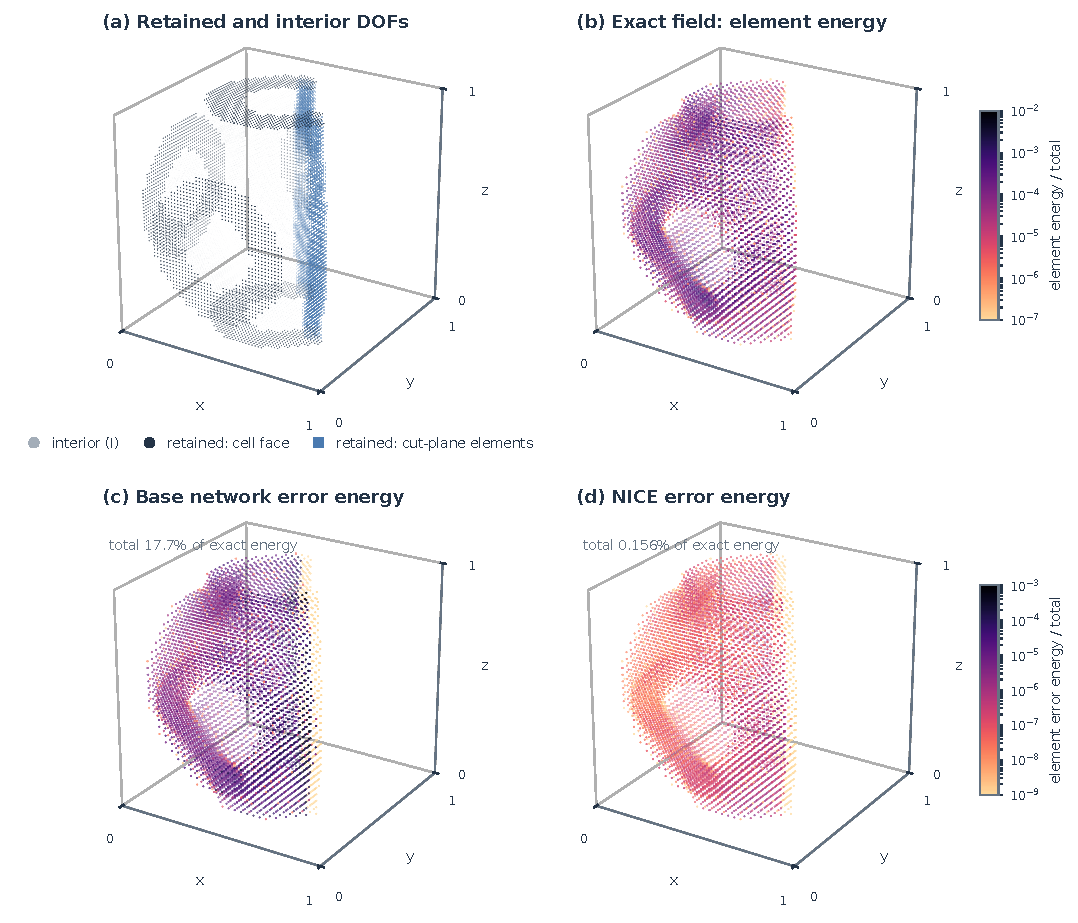
\includegraphics[width=\textwidth]{../figures/F12_field_error_M1.pdf}
\caption{\textbf{Retained coordinates and spatial distribution of the extension error in M1.} (a) Retained box-face coordinates, retained cut-band coordinates of the elements carrying the macro-cut surface, and internal coordinates. (b) Bulk element energies of the exact field under one consistent-traction direction, relative to its total. (c,d) Bulk element energies of the error of B and of the corrected predictor A3 for the same retained displacement, on a common colour scale. Elements of the cut band carry no error because their coefficients are retained.}\label{fig:7}
\end{figure}

The magnitude of these energy errors reflects an amplification that can be measured directly. For a direction with interior error \(d_I\) and exact interior field \(u_I\), write \(\delta^2=d_I^TDd_I/u_I^TDu_I\) for the Jacobi-weighted relative displacement error and \(\kappa=R(d)/R(u)\) for the ratio of the Rayleigh quotients \(R(d)=d_I^TAd_I/d_I^TDd_I\) and \(R(u)=u^TKu/u_I^TDu_I\). Then the relative energy excess is exactly \(\varepsilon=\delta^2\kappa\). Under consistent tractions, B\textquotesingle s fields in M1, M2, H1 and H2 have \(\delta\) of 0.7--1.3\% but \(\kappa\) of 124 to 7089: the displacement error is small, yet it lies in directions that are far stiffer, relative to their amplitude, than the exact field, which in these thin-walled cells deforms mainly through soft bending of the walls. A displacement accuracy of about one percent therefore produces energy errors of 2--35\%; in the uncut U2 the same \(\delta\) of 0.74\% meets \(\kappa=85\) and gives only 0.40\%. The correction acts on both factors: A3\textquotesingle s fields have \(\delta\) of 0.05--0.19\% and \(\kappa\) of 33 to 582 in the cut cells (0.11\% and 47 in U2), so that the stiff error components, which relaxation removes efficiently, no longer dominate.

Thickness sensitivity introduces the derivative weighting in Eq. (13). At fixed retained displacement, M1 has mean energy and field-based sensitivity errors of 13.5\% and 14.1\%, whereas H2 has errors of 35\% and 75.1\%, respectively, under consistent tractions. The linear term contributes only 7.2\% and 0.79\% of the sum of the linear- and quadratic-term norms, evaluated jointly over the eight thickness parameters and the applied directions. The quadratic contribution therefore dominates these finite-error examples. The linear term in the expansion remains relevant as the error changes in magnitude and alignment. Table ST02 and Figure S03 show how this balance varies across cells and direction classes.

\subsection{Reducing interior error with fixed network weights}

Holding B fixed isolates the effect of equilibrium correction from changes in the learned weights. We first apply Chebyshev smoothing to five cells under nodal-force and consistent-traction directions, preserving the same retained displacement throughout. A zero interior field with those retained values provides a comparison for the contribution of the learned starting field.

Eight smoothing steps reduce the mean energy excess in every cell and loading class, but the residual errors differ strongly (Figure 8). Under consistent tractions, H2 decreases from 35\% to 0.205\%, while M1 decreases from 13.5\% to 4.68\%. At 32 steps the corresponding errors are 0.00333\% and 2.95\%. This contrast is consistent with the spectral locations in Section 6.4: much of M1\textquotesingle s low-mode error lies below the interval targeted by the smoother. M1\textquotesingle s mean field-based sensitivity error decreases from 14.1\% to 2.76\% after eight steps, although its evolution between these endpoints is not monotone (Figure S02A). At 32 steps, the learned starting field gives lower energy excess than the zero interior field in all the cases considered. Table ST03 gives both initialisations and the directional percentiles.

An interior coarse correction addresses the error that remains after relaxation. On M1, adding a trilinear coarse correction before the same eight-step smoothing stage reduces the mean energy excess from 4.68\% to 0.230\%. Adding eight pre-smoothing steps lowers it further to 0.186\%, compared with 13.5\% before correction. The first comparison holds the smoothing count fixed and identifies the additional benefit of the coarse update, whose solve contributes extra work. The \(Q_1(17)\) correction uses 5,601 coarse coefficients for 165,927 internal degrees of freedom. Applying the complete eight-step/coarse/eight-step cycle to M2 and U1 gives approximately 0.027\% under the same loading class.

The remaining error can be varied through the correction budget. On M1, two, four and eight smoothing steps on each side of the trilinear coarse update give 1.02\%, 0.422\% and 0.186\%, respectively. These fixed-weight results establish the local accuracy benefit of combining smoothing and coarse correction while preserving the retained representation. Quadratic interpolation and zero-field comparisons are given in Figure S02B and Table ST04, with Appendix F.1 describing their coarse representations; enriched partition-of-unity spaces are recorded there as numerical observations only (Supplementary Note S6).

What does the learned field contribute once the correction is applied? Table 3 applies the same correction to four starting fields at the same retained displacements: a zero interior, a graph-harmonic interior extension, B\textquotesingle s learned field, and, for reference, A3. The zero and harmonic fields receive the same exact rigid-body split as the network. With eight smoothing steps on each side of the coarse solve, a zero interior leaves 28--1100\% energy excess and the harmonic extension 0.08--17\%, whereas B\textquotesingle s field ends at 0.004--0.19\%, lower than the harmonic start by factors of 7 to 290. Quadrupling the smoothing budget to 32 steps per stage does not close the gap: the harmonic start then reaches 0.0006--4.1\%, still above B\textquotesingle s field at the eight-step budget in four of the five cells. The learned field therefore supplies the part of the interior equilibrium that the smoothing and the coarse space do not reach at a practical budget, chiefly the slowly relaxed components identified in Section 6.4. Table ST18 gives both loading classes.

{\small
\begin{longtable}[]{@{}llrrrr@{}}
\caption{Mean energy excess (\%) after the same correction applied to different starting fields (consistent tractions, 32 directions).}\tabularnewline
\toprule\noalign{}
Cell & Correction & Zero interior & Harmonic & B (learned) & A3 \\
\midrule\noalign{}
\endfirsthead
\toprule\noalign{}
Cell & Correction & Zero interior & Harmonic & B (learned) & A3 \\
\midrule\noalign{}
\endhead
\bottomrule\noalign{}
\endlastfoot
M1 & 8 / \(Q_1(17)\) / 8 & 1097 & 17.2 & 0.186 & 0.131 \\
M1 & 32 / \(Q_1(17)\) / 32 & 185 & 4.11 & 0.0727 & --- \\
M2 & 8 / \(Q_1(17)\) / 8 & 324 & 6.72 & 0.0273 & 0.0358 \\
M2 & 32 / \(Q_1(17)\) / 32 & 38.9 & 1.52 & 0.00691 & --- \\
H1 & 8 / \(Q_1(17)\) / 8 & 39.9 & 1.28 & 0.0131 & 0.0115 \\
H1 & 32 / \(Q_1(17)\) / 32 & 2.92 & 0.199 & 0.00130 & --- \\
H2 & 8 / \(Q_1(17)\) / 8 & 28.3 & 0.0806 & 0.0117 & 0.0148 \\
H2 & 32 / \(Q_1(17)\) / 32 & 0.0156 & 0.000614 & 0.000182 & --- \\
U2 & 8 / \(Q_1(17)\) / 8 & 47.2 & 1.23 & 0.00424 & 0.00465 \\
U2 & 32 / \(Q_1(17)\) / 32 & 5.51 & 0.380 & 0.00090 & --- \\
\end{longtable}}

Uncorrected, B\textquotesingle s errors in these cells are 13.5\% (M1), 3.64\% (M2), 1.81\% (H1), 35\% (H2) and 0.402\% (U2). The harmonic extension solves a graph Laplacian on the element connectivity weighted by material volume; its setup cost is one sparse factorisation of that Laplacian. The comparison also shows that, locally, applying the correction to B\textquotesingle s unchanged weights (B+W) is about as accurate as the predictor trained through the correction: A3 is lower on M1 and H1 and higher on M2, H2 and U2. The assembled comparison in Section 6.6 shows the same pattern for the structural responses: the correction alone suffices for the accuracy reference, and training through it lowers the largest sensitivity errors by factors of up to 2.2.

\begin{figure}[!htbp]
\centering
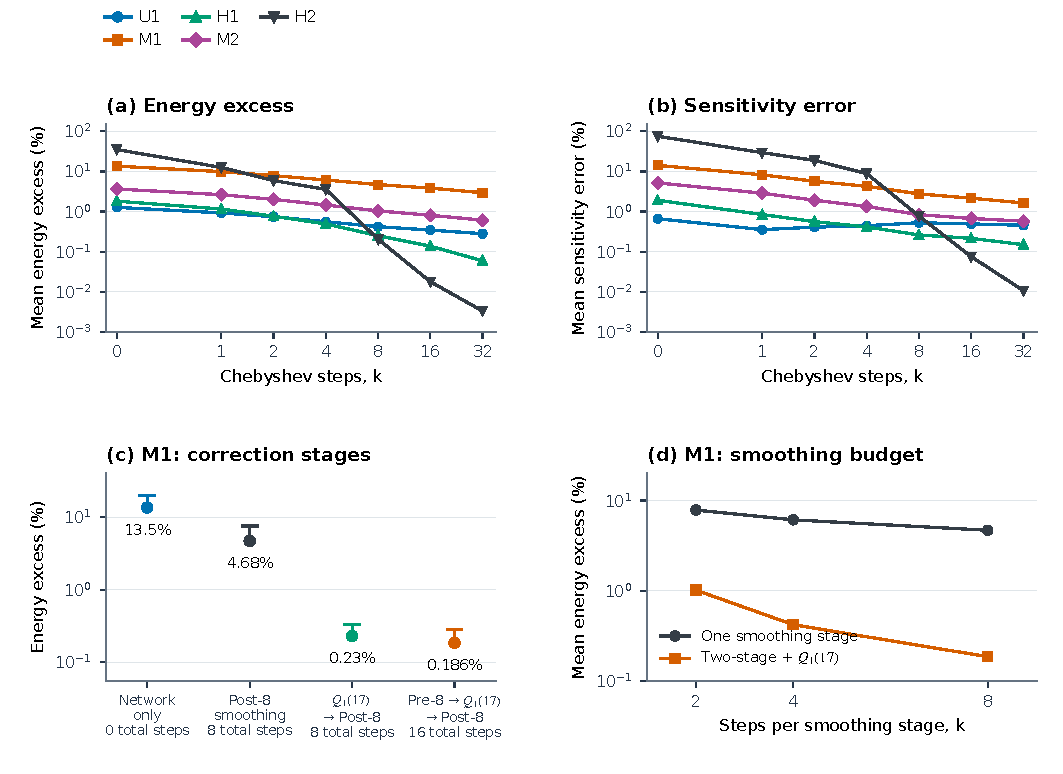
\includegraphics[width=\textwidth]{../figures/F04_correction.pdf}
\caption{\textbf{Accuracy gained by correcting B at fixed weights.} (a,b) Mean directional energy excess and field-based sensitivity error during Chebyshev smoothing on five cells. (c) M1 with no correction, eight smoothing steps, coarse correction followed by eight steps, and eight steps on each side of the coarse correction. The mean excesses are 13.5\%, 4.68\%, 0.230\% and 0.186\%, with 0, 8, 8 and 16 smoothing steps in total. Dots show means and caps the 90th percentile. The two methods with eight smoothing steps differ by one additional coarse solve. The \(Q_1(17)\) representation contains 5,601 coefficient columns for 165,927 internal degrees of freedom. (d) Mean energy excess versus steps per smoothing stage; the complete cycle uses twice this count. All panels use consistent tractions, fixed retained displacements and \(a=b/30\). In (a,b), the step axis is linear from zero to one and logarithmic thereafter.}\label{fig:8}
\end{figure}

\subsection{Compliance and local sensitivity after assembly}

Assembly places different accuracy demands on global work and local design quantities. Figure 9 compares the predictors in the two-cell configurations of Figure 4, with an exact neighbour in every case, using 3\% on compliance and on each cell\textquotesingle s eight-parameter sensitivity vector as a common accuracy reference. The principal predictor meets both requirements in all fourteen configurations evaluated: its largest compliance error over the six face loads is 0.056\% (M1/x) and its largest sensitivity error, taken over both cells, is 0.67\% (U1/y). The uncorrected continuation C was evaluated on eleven configurations, the nine common to all predictors and L1/x and L1/y; it fails the sensitivity requirement in four of them (U1/x, U1/y, M1/x, M1/y, with up to 11.4\%), and S8 fails in the same four of the nine common configurations (up to 5.83\%). Table ST13 lists the configuration maxima of all predictors, and Table ST06 the cut-traction responses. A2b, trained through the smoothing alone, reduces these errors but still fails the same four configurations (3.15--4.43\%): smoothing without the coarse solve does not reach the slowly relaxed error components that dominate the sensitivity of U1 and M1. B+W, which applies A3\textquotesingle s complete correction to B\textquotesingle s unchanged weights, also meets both requirements in the same fourteen configurations, with a largest sensitivity error of 0.95\% (U1/x). The correction is therefore what brings the assembled responses within the accuracy reference; training through it reduces the remaining sensitivity error on the most demanding cells, from 0.35\% to 0.16--0.21\% on M1 and from 0.90--0.95\% to 0.60--0.67\% on U1, while on M2 the untrained combination is marginally more accurate. On the lightly cut L1, whose exact two-cell reference exceeds the device memory and was therefore formed and factorised on the host, A3 gives at most 0.0020\% in compliance and 0.10\% in sensitivity, B+W 0.0019\% and 0.087\%, and C 0.18\% and 1.9\%: all three meet the reference there, in line with the small errors of lightly cut cells in Section 6.3.

The load-specific responses show why both quantities are needed, and how the correction changes their relation. For the uncorrected and partially corrected predictors, an accurate compliance does not guarantee an accurate local sensitivity: under a neighbour-face load on U1/x, S8\textquotesingle s compliance error is 0.00137\% while the target-cell sensitivity error is 3.89\%, with the target carrying 0.13\% of the exact assembled energy. A3 reduces both errors under the same loads (Table 4): the target-cell sensitivity error of that load falls to 0.598\%, and on M1/x, the configuration with the largest errors for C and S8, the target-face y load gives 0.0481\% and 0.145\% instead of 1.42\% and 5.83\%. The separation between global and local accuracy therefore remains visible in A3, in that its sensitivity error exceeds its compliance error by a factor of about two for a target-face load on the heavily cut H1 and by four orders of magnitude for the weakly participating U1 target, but both now lie well within the accuracy reference. Sections 6.7 and 7.2 explain this separation through energy participation and the derivative weighting of the sensitivity.

\begin{figure}[!htbp]
\centering
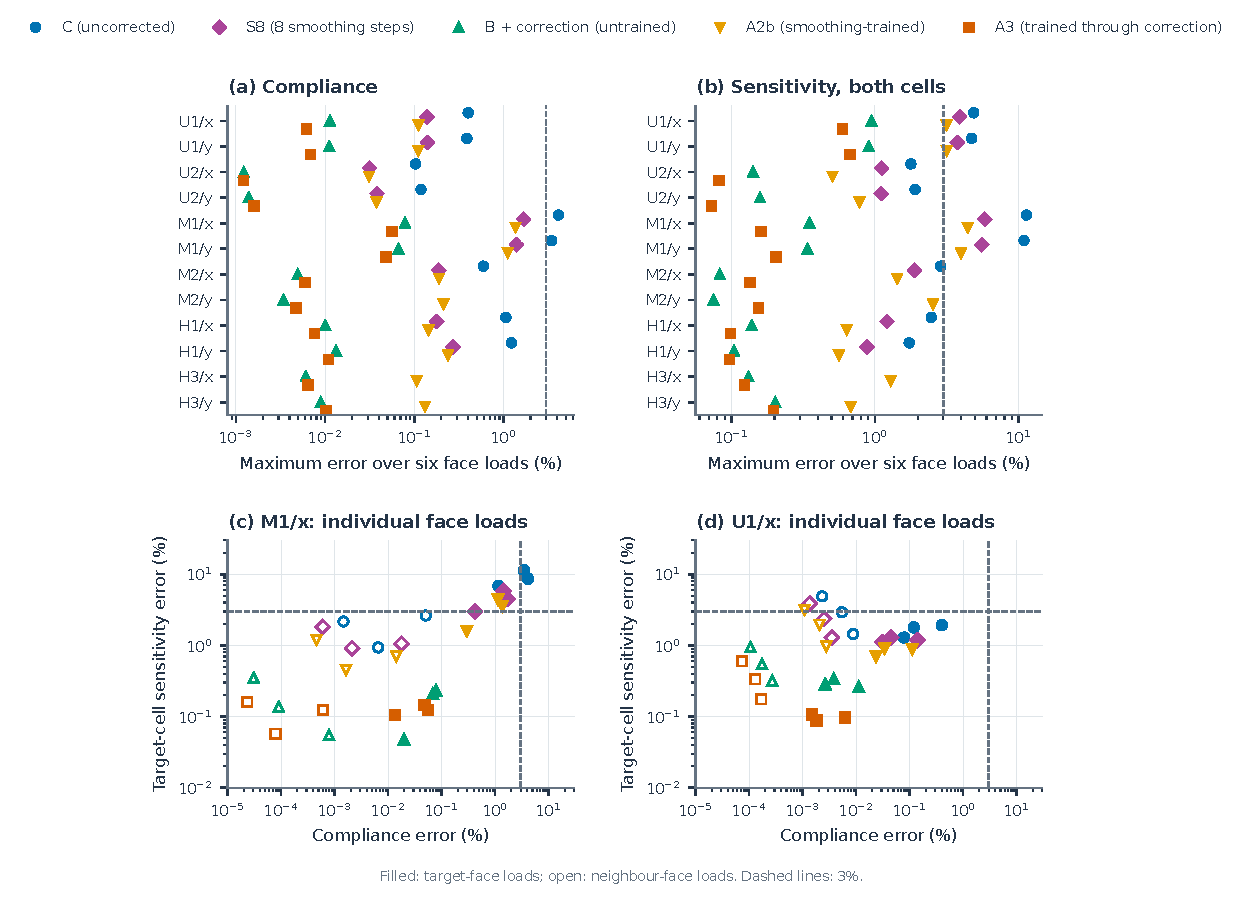
\includegraphics[width=\textwidth]{../figures/F05_assembly_A3.pdf}
\caption{\textbf{Compliance and thickness sensitivity in assembled cell pairs.} The target cell uses a learned operator and the neighbour exact condensation. (a,b) Maximum errors over the six face loads in each configuration; the sensitivity error is also maximised over both cells. (c,d) Compliance and target-cell sensitivity errors of the individual face loads on M1/x and U1/x; filled markers denote target-face loads and open markers neighbour-face loads. Dashed lines mark 3\%. The uncorrected predictor C reaches sensitivity errors of 4.7--11.4\% in four configurations and A2b, trained through smoothing alone, 3.2--4.4\% in the same four; the principal predictor A3 stays below 0.06\% in compliance and 0.67\% in sensitivity in all fourteen configurations. H3 is a further heavily cut cell evaluated for A2b, B+W and A3 only. B+W was evaluated on the same fourteen configurations as A3; L1 is a lightly cut cell evaluated for C, B+W and A3.}\label{fig:9}
\end{figure}

{\footnotesize
\begin{longtable}[]{@{}
  >{\raggedright\arraybackslash}p{(\linewidth - 10\tabcolsep) * \real{0.1579}}
  >{\raggedright\arraybackslash}p{(\linewidth - 10\tabcolsep) * \real{0.1579}}
  >{\raggedright\arraybackslash}p{(\linewidth - 10\tabcolsep) * \real{0.1579}}
  >{\raggedright\arraybackslash}p{(\linewidth - 10\tabcolsep) * \real{0.1579}}
  >{\raggedright\arraybackslash}p{(\linewidth - 10\tabcolsep) * \real{0.1579}}
  >{\raggedleft\arraybackslash}p{(\linewidth - 10\tabcolsep) * \real{0.2105}}@{}}
\caption{Compliance and target-cell sensitivity under individual face loads.}\tabularnewline
\toprule\noalign{}
\begin{minipage}[b]{\linewidth}\raggedright
Target / configuration
\end{minipage} & \begin{minipage}[b]{\linewidth}\raggedright
Load
\end{minipage} & \begin{minipage}[b]{\linewidth}\raggedright
C: compliance / sensitivity (\%)
\end{minipage} & \begin{minipage}[b]{\linewidth}\raggedright
S8: compliance / sensitivity (\%)
\end{minipage} & \begin{minipage}[b]{\linewidth}\raggedright
A3: compliance / sensitivity (\%)
\end{minipage} & \begin{minipage}[b]{\linewidth}\raggedleft
Target energy share
\end{minipage} \\
\midrule\noalign{}
\endfirsthead
\toprule\noalign{}
\begin{minipage}[b]{\linewidth}\raggedright
Target / configuration
\end{minipage} & \begin{minipage}[b]{\linewidth}\raggedright
Load
\end{minipage} & \begin{minipage}[b]{\linewidth}\raggedright
C: compliance / sensitivity (\%)
\end{minipage} & \begin{minipage}[b]{\linewidth}\raggedright
S8: compliance / sensitivity (\%)
\end{minipage} & \begin{minipage}[b]{\linewidth}\raggedright
A3: compliance / sensitivity (\%)
\end{minipage} & \begin{minipage}[b]{\linewidth}\raggedleft
Target energy share
\end{minipage} \\
\midrule\noalign{}
\endhead
\bottomrule\noalign{}
\endlastfoot
H1/x & T-x & 1.06 / 2.47 & 0.178 / 1.22 & 0.0076 / 0.0133 & 0.643 \\
U1/x & N-z & 0.0023 / 4.89 & 0.00137 / 3.89 & 7.3×10⁻⁵ / 0.598 & 0.0013 \\
M1/x & T-y & 3.44 / 11.4 & 1.42 / 5.83 & 0.0481 / 0.145 & 0.311 \\
\end{longtable}}

The target uses the learned operator and the neighbour exact condensation. T and N identify the loaded face; x, y and z give the traction direction. Each row compares the two response errors for the same load; the last column gives the target cell\textquotesingle s share of the exact assembled energy. H1 is heavily cut, M1 moderately cut and U1 uncut. Configuration-level sensitivity maxima include both cells.

\subsection{Energy participation and field recovery}

Energy participation explains how a local stiffness error can have a small effect on global compliance. Under the neighbour-face z load in U1/x, B\textquotesingle s target cell carries 0.127\% of the exact assembled energy and has a local directional energy excess of 2.31\%. Their product, \(\beta=w\varepsilon\), gives a relative compliance bound of 0.00295\%, close to the observed 0.00283\%. The target-cell sensitivity error is nevertheless 5.83\%. Figure 10 shows this participation weighting across the finite load responses. Equation (12) relates the local energy error to global work, while Eq. (J.4) relates local relative sensitivity error to participation, derivative coupling and the local reference scale.

Sensitivity further depends on the interaction between field recovery and the assembled retained displacement. For B on M1/x under the target-face y load, the full sensitivity error is 12.2\%. Evaluating the learned extension at the exact retained displacement gives 15.6\%, whereas evaluating the exact extension at the learned retained displacement gives 19.3\% (Table ST05). The full error is smaller than either replacement error. The vector expansion in Eq. (H.2) accounts for this interaction: the extension error, the retained-displacement change and their mixed term enter the recovered field together. The replacement norms consequently cannot be added as scalar error contributions. Table ST05 gives the replacement results, and Tables ST15--ST16 give the load-specific responses for S8 and B.

\begin{figure}[!htbp]
\centering
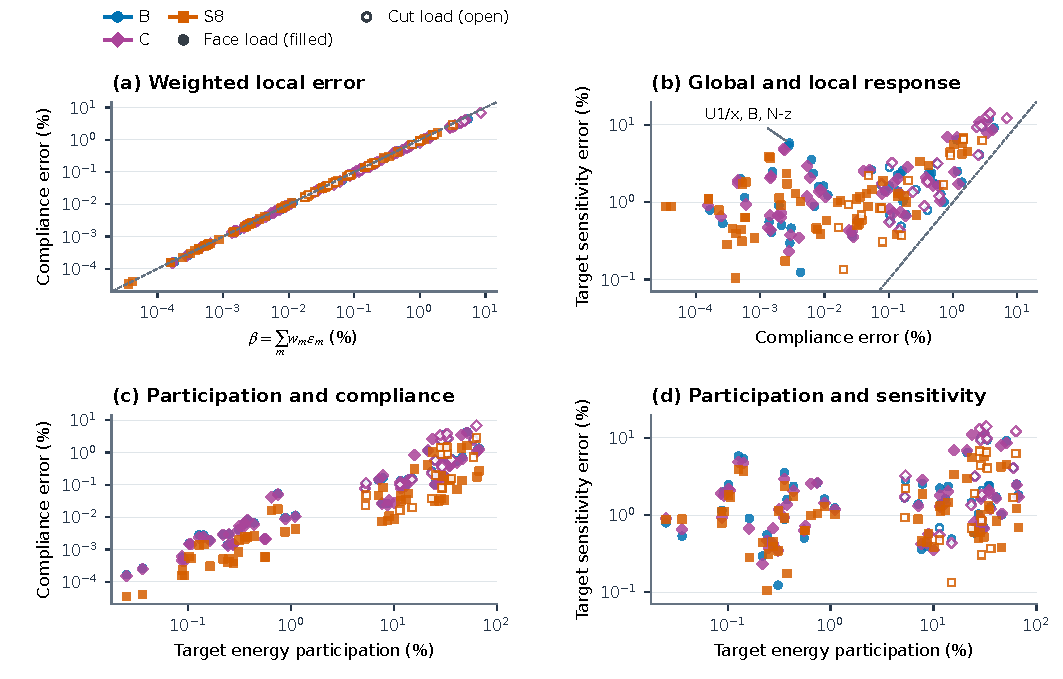
\includegraphics[width=\textwidth]{../figures/F10_energy_participation.pdf}
\caption{\textbf{Participation-weighted compliance error and local sensitivity.} Each point is one load for one model--configuration combination: 192 observations from the 25 B, C and S8 model--configuration combinations of Table ST13 other than L1. Filled markers denote face loads and open markers macro-cut loads. (a) Compliance error against \(\beta=\sum_mw_m\varepsilon_m\), with \(w_m=q_m^TS_mq_m/C\) and \(\varepsilon_m=q_m^T(\widehat S_m-S_m)q_m/(q_m^TS_mq_m)\), evaluated at the exact assembled retained displacement. Only the learned target contributes to \(\beta\). (b) Compliance and target-cell sensitivity errors under the same loads; the annotation identifies B on U1/x under the neighbour-z load. Dashed lines in (a,b) denote equality. (c,d) The two response errors versus the target\textquotesingle s exact energy participation.}\label{fig:10}
\end{figure}

\subsection{Effect of restricting the retained representation}

A complementary comparison isolates the effect of restricting the retained representation, as substructures with interpolated boundary displacements do \href{https://doi.org/10.1016/j.eml.2023.102041}{Huang et al. (2023)}, \href{https://doi.org/10.1016/j.cma.2026.118955}{Guo et al. (2026a)}. Pairs in configuration x are solved with exact cell operators while the box-face displacements are restricted to tensor Bernstein polynomials of degree \(r\) over each cell; degree one on the eight corners corresponds to the corner-linear boundary interpolation of the three-dimensional PIML examples. The non-box cut-band coordinates remain unrestricted, which favours the restricted model. Two variants are examined: every box face restricted, as in a lattice built entirely from such substructures, and only the shared interface restricted.

With every box face restricted, the corner-linear boundary gives compliance errors of 78--85\% on U1, M1, M2 and H1 (Figure 11). The error decreases with degree to about 4\% at \(r=5\) and 0.49--0.74\% at \(r=8\), where the restricted problem retains, on H1, 14,001 of 32,991 free coordinates. The local sensitivity converges more slowly: at \(r=8\) the maximum target-cell sensitivity error is 1.3--4.5\% over the target-face loads and 24--64\% when neighbour-face loads are included, the latter because the loads applied to the neighbour deform the shared face in patterns that a polynomial of degree eight does not resolve. Restricting only the shared interface removes most of the compliance error (U1, M1 and M2: 1.95--9.4\% at \(r=1\), 0.17--0.44\% at \(r=3\)), but the sensitivity error under neighbour loads remains 8--21\% at \(r=3\) and 2.2--3.4\% at \(r=5\). These maxima refer to their respective load sets and need not occur under the same load. The separation between global and local accuracy thus persists, and is stronger, when the approximation enters through the retained space; the full retained representation used here avoids it by construction. Table ST07 gives the degree sweeps and cut-traction responses.

\begin{figure}[!htbp]
\centering
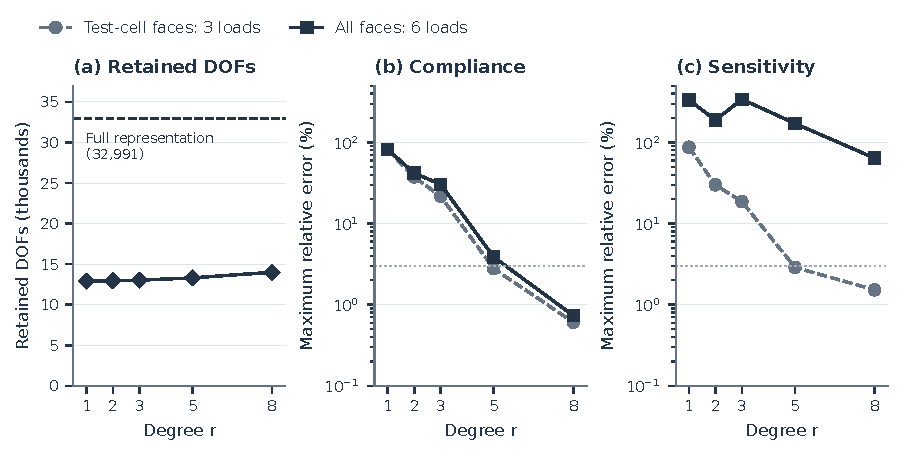
\includegraphics[width=\textwidth]{../figures/F06_bernstein.pdf}
\caption{\textbf{Response errors caused by restricting box-face displacements.} Both cells of H1/x use exact operators and Bernstein degree \(r\) on every box face, with unrestricted non-box cut-band coordinates. (a) Reduced coordinate count; the dashed line denotes the 32,991-coordinate full representation. (b,c) Maximum compliance and target-cell sensitivity errors over the three target-face loads or all six target- and neighbour-face loads. Macro-cut tractions are excluded from both sets. Errors are relative to the full retained-space solution; horizontal reference lines mark 3\%.}\label{fig:11}
\end{figure}

\subsection{Heterogeneous lattices with every cell learned}

The two-cell examples isolate one learned cell. In a design, every cell of the lattice is represented by the learned operator, and the errors of neighbouring cells enter the same assembled solution. Two lattices with a continuous graded thickness field and a planar boundary cut test this situation: a \(2\times2\times2\) block of eight distinct cells, four of them cut with retained volumes of 62\% and 25\%, and a \(3\times3\times1\) layer of eight cells, with one corner position left empty and three of the cells cut. Corner parameters range from 0.25 to 0.56 and neighbouring cells share their face corners. The lattices are clamped on one face and loaded by unit consistent tractions on the opposite face; every cell uses the learned operator, and the reference assembles the exact condensation of every cell. The reference holds no interior factorisation during the assembled solve: the dense condensed matrix of each cell is formed on its own, and the retained-level system is solved with these matrices to a recomputed relative residual of \(9\times10^{-11}\). Three random load vectors complement the three consistent face loads.

In the \(2\times2\times2\) block, with all eight cells represented by A3, the lattice compliance errors under the three consistent face loads are 0.014\%, 0.011\% and 0.0094\%, and at most 0.069\% under the random loads. The largest eight-corner sensitivity error over all cells is 0.14\% under the consistent loads and 0.45\% under the random loads, and the assembled retained solution differs from the exact one by 0.13\%. These errors are smaller than the largest errors of the two-cell configurations with a single learned cell (Section 6.6): the energy errors of the individual cells combine through their shares of the assembled energy rather than accumulate. The learned solve reaches the prescribed recursive residual, while its recomputed residual stagnates at \(3.6\times10^{-4}\), the level set by the network\textquotesingle s single-precision arithmetic; the errors above are measured at this solution. The \(3\times3\times1\) layer, with five uncut and three cut cells, behaves in the same way: the compliance errors are 0.015\%, 0.013\% and 0.010\% under the consistent loads and at most 0.056\% under the random loads, the largest sensitivity error is 0.14\% under the consistent loads (0.43\% under the random loads), and the retained solution differs by 0.12\%; the recomputed residual of the learned solve stagnates at \(3.2\times10^{-3}\).

By Eq. (12), the compliance errors of the learned cells add with the same sign, so the lattice compliance error is bounded by the participation-weighted sum of the cells\textquotesingle{} energy errors at the exact traces. The measured errors follow this bound closely. The cells\textquotesingle{} own energy errors at the exact traces range from 0.03\% to 0.12\%, largest in the cut cells; weighted by the cells\textquotesingle{} shares of the assembled energy, their sums are 0.014\%, 0.011\% and 0.0094\% for the consistent loads, exceeding the lattice compliance errors by less than 0.3\% of their value, and 4--5\% above them for the random loads. The difference arises because the assembled retained solution relaxes towards the stiffer surrogate, whereas \(\beta\) evaluates the cells\textquotesingle{} errors at the exact traces; it is small because the assembled retained displacements differ little from the exact ones. In the \(3\times3\times1\) layer the cells\textquotesingle{} energy errors range from 0.03\% to 0.08\%, and the weighted sums exceed the lattice compliance errors by less than 0.4\% for the consistent loads and by 4--5\% for the random loads.

\subsection{Computational cost against conventional condensation}

The practical alternative to a learned substructure is the conventional route: assemble the cut finite element stiffness of each cell and condense its interior with a sparse direct solver, either forming the dense condensed matrix \(S\) or applying it through the interior factorisation. Both routes share the geometric preprocessing, the cut-cell integration and the stiffness assembly, because the learned operator also evaluates \(F^TKF\) with the exact stiffness. They differ in the condensation: an interior factorisation, and for the explicit variant one solve per retained coordinate, against the network\textquotesingle s geometry encoding, the smoothing-interval estimate and coarse factorisation of the correction, and the forward and transpose actions per query.

Table 5 compares the two routes on the four deployment cells, two cut and two uncut, with 67,224 to 404,148 degrees of freedom. The conventional route runs on the 16 host cores available to the job (MKL PARDISO, 16 threads), as a practitioner would condense a cell; the learned route runs on one RTX 5090. Geometry preprocessing is identical for both routes; cell setup, moment integration and stiffness assembly use the same implementation, on the host cores for the conventional route and on the GPU for the learned route.

\begin{landscape}
{\scriptsize
\begin{longtable}[]{@{}
  >{\raggedright\arraybackslash}p{(\linewidth - 14\tabcolsep) * \real{0.090}}
  >{\raggedright\arraybackslash}p{(\linewidth - 14\tabcolsep) * \real{0.150}}
  >{\raggedright\arraybackslash}p{(\linewidth - 14\tabcolsep) * \real{0.110}}
  >{\raggedright\arraybackslash}p{(\linewidth - 14\tabcolsep) * \real{0.130}}
  >{\raggedright\arraybackslash}p{(\linewidth - 14\tabcolsep) * \real{0.130}}
  >{\raggedright\arraybackslash}p{(\linewidth - 14\tabcolsep) * \real{0.160}}
  >{\raggedright\arraybackslash}p{(\linewidth - 14\tabcolsep) * \real{0.190}}
  >{\raggedright\arraybackslash}p{(\linewidth - 14\tabcolsep) * \real{0.120}}@{}}
\caption{Cost per cell of the conventional and learned routes. Front end: geometry preprocessing plus cell setup, moment integration and stiffness assembly. Condensation: interior factorisation for the conventional route; network encoding plus correction setup (smoothing interval and coarse factorisation) for the learned route. Memory: interior factor, or the learned operator\textquotesingle s stored state. Application: \(Sq\) or \(\widehat Sq\) for a batch of 1, 16 or 64 retained vectors. Explicit \(S\): dense condensed matrix by one host solve per retained coordinate (timed for 300 s and extrapolated linearly in the number of columns where marked *). Host timings on an otherwise idle job; a first run with other jobs sharing the host cores agreed within 10\% for G1--G3.}\tabularnewline
\toprule\noalign{}
\begin{minipage}[b]{\linewidth}\raggedright
Cell
\end{minipage} & \begin{minipage}[b]{\linewidth}\raggedright
DOFs / retained
\end{minipage} & \begin{minipage}[b]{\linewidth}\raggedright
Front end (s): host / GPU
\end{minipage} & \begin{minipage}[b]{\linewidth}\raggedright
Condensation (s): learned / host PARDISO
\end{minipage} & \begin{minipage}[b]{\linewidth}\raggedright
Memory (GB): learned / host
\end{minipage} & \begin{minipage}[b]{\linewidth}\raggedright
Application, 1 / 16 / 64 vectors (ms): learned
\end{minipage} & \begin{minipage}[b]{\linewidth}\raggedright
host PARDISO
\end{minipage} & \begin{minipage}[b]{\linewidth}\raggedright
Explicit \(S\), host (s / GB)
\end{minipage} \\
\midrule\noalign{}
\endfirsthead
\toprule\noalign{}
\begin{minipage}[b]{\linewidth}\raggedright
Cell
\end{minipage} & \begin{minipage}[b]{\linewidth}\raggedright
DOFs / retained
\end{minipage} & \begin{minipage}[b]{\linewidth}\raggedright
Front end (s): host / GPU
\end{minipage} & \begin{minipage}[b]{\linewidth}\raggedright
Condensation (s): learned / host PARDISO
\end{minipage} & \begin{minipage}[b]{\linewidth}\raggedright
Memory (GB): learned / host
\end{minipage} & \begin{minipage}[b]{\linewidth}\raggedright
Application, 1 / 16 / 64 vectors (ms): learned
\end{minipage} & \begin{minipage}[b]{\linewidth}\raggedright
host PARDISO
\end{minipage} & \begin{minipage}[b]{\linewidth}\raggedright
Explicit \(S\), host (s / GB)
\end{minipage} \\
\midrule\noalign{}
\endhead
\bottomrule\noalign{}
\endlastfoot
G1 (cut) & 177,507 / 24,636 & 18.7 / 5.3 & 0.72 / 7.7 & 0.74 / 5.56 & 54 / 531 / 923 & 826 / 2,589 / 5,811 & 1,192* / 4.5 \\
G2 (cut) & 67,224 / 18,858 & 8.5 / 3.0 & 0.16 / 1.4 & 0.25 / 1.10 & 25 / 205 / 388 & 184 / 475 / 1,023 & 247 / 2.7 \\
G3 (uncut) & 289,494 / 17,508 & 30.3 / 6.1 & 0.78 / 19.2 & 1.20 / 12.3 & 84 / 877 / 1,481 & 1,783 / 5,582 / 8,987 & 1,609* / 2.3 \\
G4 (uncut) & 404,148 / 25,920 & 30.1 / 6.5 & 1.09 / 31.3 & 1.37 / 18.5 & 99 / 1,052 / 1,828 & 2,264 / 7,953 / 12,849 & 3,566* / 5.0 \\
\end{longtable}}
\end{landscape}


Against the conventional route, the learned operator condenses a cell 8.8 to 29 times faster and stores 4.4 to 13.5 times less. Each subsequent application is 7.4 to 23 times faster for a single vector and 2.3 to 7.6 times faster for batches of 16 or 64 vectors: the host solves are limited by reading the factor from memory, and the factor grows faster than the retained dimension. Forming the dense condensed matrix on the host takes 4 to 59 minutes per cell, against an estimated 2 to 12 minutes for evaluating \(\widehat S\) on all retained unit vectors in batches of 64. Including geometry preprocessing and assembly, a cell is ready for queries after 3.2 to 7.6 s on the learned route and 9.9 to 61 s on the conventional route, a factor of 3.1 to 8.1 that grows with cell size. Since both preparation and every application are cheaper, the learned route is cheaper for any number of queries per design iteration.

How many applications a design iteration requires depends on the assembled solver: in the lattices of Section 6.9, the preconditioned iteration needs 183 applications per cell with the exact cells and 186 with the learned cells for a batch of six loads (226 and 234 in the \(3\times3\times1\) layer). Since every application is cheaper, this count does not change the comparison with the conventional route.

A further alternative avoids condensation altogether: the full cut finite element model of the lattice, with the retained and interior degrees of freedom of every cell in one global stiffness matrix, is factorised once by a sparse direct solver and solved for all loads. Table 6 compares this whole-lattice direct solution, on the same 16 host cores (MKL PARDISO), with one design iteration of the learned route on the GPU. Besides the two eight-cell lattices of Section 6.9, it includes the two \(2\times2\times1\) layers of the \(2\times2\times2\) block as four-cell lattices, each with two uncut cells and two cut cells of 62\% and 25\% retained volume, clamped and loaded in the same way. The direct solution couples the cells through the same retained degrees of freedom, clamp and consistent face loads as the learned lattice, with three random loads in addition; its recomputed relative residuals are below \(10^{-10}\) for all six loads, so that for the four-cell lattices it also serves as the exact reference. The learned route is timed as deployed: front end, preconditioner setup, preconditioned conjugate gradients for the three consistent loads to a relative residual of \(10^{-6}\), and the sensitivities. The direct times include six loads but no sensitivities. Both routes start from the same generated cell geometries.

{\footnotesize
\begin{longtable}[]{@{}
  >{\raggedright\arraybackslash}p{(\linewidth - 12\tabcolsep) * \real{0.1474}}
  >{\raggedright\arraybackslash}p{(\linewidth - 12\tabcolsep) * \real{0.1474}}
  >{\raggedright\arraybackslash}p{(\linewidth - 12\tabcolsep) * \real{0.1368}}
  >{\raggedright\arraybackslash}p{(\linewidth - 12\tabcolsep) * \real{0.1368}}
  >{\raggedright\arraybackslash}p{(\linewidth - 12\tabcolsep) * \real{0.1368}}
  >{\raggedright\arraybackslash}p{(\linewidth - 12\tabcolsep) * \real{0.1263}}
  >{\raggedright\arraybackslash}p{(\linewidth - 12\tabcolsep) * \real{0.1684}}@{}}
\caption{Whole-lattice direct solution on the host versus the learned route. Direct: every cell\textquotesingle s full cut-cell stiffness in one global matrix, factorised by MKL PARDISO on 16 host cores; time from cell setup and assembly on the host to the solution for six loads (three consistent, three random); memory: PARDISO\textquotesingle s permanent and factorisation storage. For the eight-cell lattices the factorisation was not run: time up to the symbolic analysis, memory as predicted by the analysis. Learned: one design iteration of the deployed route on one RTX 5090 (front end, preconditioner setup, conjugate-gradient solve for the three consistent loads to \(10^{-6}\), sensitivities); GPU memory at its peak, host memory after the front end. Compliance error of the learned route under the three consistent loads, against the direct solution (four cells) or the exact condensation of Section 6.9 (eight cells); the learned compliance lies below the reference in every case. Table ST20 gives all phases.}\tabularnewline
\toprule\noalign{}
\begin{minipage}[b]{\linewidth}\raggedright
Lattice (cut / cells)
\end{minipage} & \begin{minipage}[b]{\linewidth}\raggedright
DOFs: total / free retained
\end{minipage} & \begin{minipage}[b]{\linewidth}\raggedright
Direct, Cholesky: time (s) / memory (GB)
\end{minipage} & \begin{minipage}[b]{\linewidth}\raggedright
Direct, LU: time (s) / memory (GB)
\end{minipage} & \begin{minipage}[b]{\linewidth}\raggedright
Learned: time (s) / iterations
\end{minipage} & \begin{minipage}[b]{\linewidth}\raggedright
Learned memory (GB): GPU / host
\end{minipage} & \begin{minipage}[b]{\linewidth}\raggedright
Learned compliance error (\%)
\end{minipage} \\
\midrule\noalign{}
\endfirsthead
\toprule\noalign{}
\begin{minipage}[b]{\linewidth}\raggedright
Lattice (cut / cells)
\end{minipage} & \begin{minipage}[b]{\linewidth}\raggedright
DOFs: total / free retained
\end{minipage} & \begin{minipage}[b]{\linewidth}\raggedright
Direct, Cholesky: time (s) / memory (GB)
\end{minipage} & \begin{minipage}[b]{\linewidth}\raggedright
Direct, LU: time (s) / memory (GB)
\end{minipage} & \begin{minipage}[b]{\linewidth}\raggedright
Learned: time (s) / iterations
\end{minipage} & \begin{minipage}[b]{\linewidth}\raggedright
Learned memory (GB): GPU / host
\end{minipage} & \begin{minipage}[b]{\linewidth}\raggedright
Learned compliance error (\%)
\end{minipage} \\
\midrule\noalign{}
\endhead
\bottomrule\noalign{}
\endlastfoot
\(2\times2\times1\), \(z=0\) (2 / 4) & 957,888 / 77,310 & 256 / 32.1 & 333 / 63.6 & 38.6 / 114 & 6.8 / 2.5 & 0.015, 0.012, 0.010 \\
\(2\times2\times1\), \(z=1\) (2 / 4) & 884,940 / 71,046 & 242 / 29.0 & 311 / 57.4 & 37.7 / 119 & 6.5 / 2.5 & 0.022, 0.016, 0.014 \\
\(2\times2\times2\) (4 / 8) & 1,833,474 / 139,002 & \textgreater{} 342 / 66.6 & \textgreater{} 358 / 132.3 & 81.2 / 129 & 9.1 / 4.1 & 0.014, 0.011, 0.0097 \\
\(3\times3\times1\) (3 / 8) & 2,113,611 / 143,685 & \textgreater{} 380 / 80.7 & \textgreater{} 395 / 160.5 & 110.1 / 165 & 9.9 / 4.9 & 0.015, 0.014, 0.015 \\
\end{longtable}}

For the four-cell lattices, the learned route completes a design iteration in 38 s, against 242 to 256 s for the direct Cholesky solution and 311 to 333 s for LU, the factorisation used in Table 5. Cell setup and assembly on the host account for 140 to 152 s of the direct time; the analysis, factorisation and solution alone take 91 s with Cholesky, against 30 to 31 s for the learned preconditioner setup and solve. The learned compliance agrees with the direct solution within 0.022\%. The factor memory grows slightly faster than the number of degrees of freedom, from 29 to 32 GB (Cholesky) and 57 to 64 GB (LU) for four cells to 67 to 81 GB and 132 to 160 GB for eight, and the process peak exceeded it by a further 5.2 to 6.4 GB in the four-cell runs. The eight-cell LU factorisations therefore exceed the 90 GB available to this job, and the eight-cell Cholesky factorisations, of 67 and 81 GB, were not run; direct solvers with out-of-core or distributed storage, which relax this limit, were not tested. The learned route needs at most 9.9 GB of GPU memory and 4.9 GB of host memory, and completes a design iteration of the eight-cell lattices in 81 and 110 s.

The historical deployment study of an earlier uncorrected predictor, including assembled iterative solves with several preconditioners, is retained in Supplementary Note S4.

\section{Discussion}

\subsection{Learning and correction in a fixed coupling space}

Fixing the retained coordinates gives a mechanical meaning to changes in the learned extension. The same box-face and cut-band displacements remain available to loads and assembly, while learning and correction alter the interior response associated with each input. In particular, an interior coarse space changes how equilibrium is approximated without restricting intercell compatibility. This distinction is useful for cut cells, where coefficients needed for cut-surface virtual work can belong to a band of active elements and need not form a minimal surface trace. The framework thus separates two decisions that a reduced substructure model otherwise combines: which displacement patterns neighbouring cells may exchange, and how accurately the interior responds to each of them.

Within this fixed space, the variational construction places the corrected learned extension in the classical Ritz setting: the extension selects an admissible field and the prescribed stiffness evaluates its energy. The complete transpose makes the returned force the derivative of that energy with respect to the retained displacement. Consequently, the interior energy error controls the amount by which the approximate condensed operator is too stiff, as expressed by Eq. (9). Symmetry and the rigid modes give this error a consistent mechanical structure; its magnitude is set by the quality of the interior extension. Rigid-body reconstruction and the reference nullspace assumptions remain essential to this interpretation.

The exact-operator Bernstein comparison reveals the complementary role of the retained space. Even with exact interior equilibrium, restricting box-face displacements changes the assembled response, and an order that gives accurate compliance for one load set can leave appreciable sensitivity error for another. Keeping the cut band unrestricted makes this comparison specific to box-face approximation. Boundary restriction and interior correction therefore act on different parts of the substructure model, and the response quantities of interest determine the acceptable error in each. This comparison also clarifies the relation to substructure methods that describe the boundary by a few coordinates, such as the corner-linear interpolation in the three-dimensional PIML examples \href{https://doi.org/10.1016/j.eml.2023.102041}{Huang et al. (2023)}. There the boundary description is exchanged for a much smaller coarse model, and its error is independent of how accurately the interior is learned. The present framework keeps the complete retained space and places the approximation error in the interior extension, where a better initial field or a larger correction budget reduces it. For the local thickness sensitivity of the cut cells examined, the boundary restriction produces larger errors than the interior approximation of the corrected operator (Sections 6.6 and 6.8); for structures where a compact coarse model matters more than local design quantities, the balance can differ.

\subsection{Why global work and local design error separate}

A small compliance error constrains a global energy norm of the reconstructed field error. The information this supplies about an individual cell depends on its role in the assembled response. Under the retained-coordinate loading and exact-equilibrium assumptions, Eq. (11) separates that error into orthogonal contributions from changed retained displacements and imperfect interior extension. For a uniformly scaled small extension error, the retained displacement changes at second order while the interior field can change at first order. This explains how accurate coupling displacements can accompany a less accurate recovered field.

Energy participation weights the influence of a local error on global work. Equation (12) weights a cell\textquotesingle s directional energy excess by its fraction of the exact assembled energy. Because that fraction depends on the load and neighbouring stiffnesses, the structural importance of a cell cannot be assigned from its geometry alone. A weakly participating target can contribute little to the compliance discrepancy while its local thickness-sensitivity vector remains inaccurate. The sensitivity error depends on the stiffness derivative acting on the field, and normalising by a small reference-vector norm can amplify the relative discrepancy. The matched-load comparisons expose this separation without changing the applied load between the two response measures.

The derivative weighting also explains why energy and sensitivity errors need not decrease together. The sensitivity expansion contains linear and quadratic field-error terms, whose relative size depends on error amplitude and alignment with the stiffness derivative. For the two difficult cut cells examined at the same retained displacement, the quadratic contribution dominates the measured aggregate term norms. In assembly, the changed retained displacement also interacts with the extension error, as Eq. (H.2) shows; the norms from the field-reconstruction and operator-replacement comparisons therefore need not add to the full sensitivity-error norm. The same separation motivates the sensitivity term of the training objective in Eq. (8): the energy term controls the interior error in the norm that governs compliance, whereas the sensitivity term weights it by the stiffness derivative that governs the local design quantities.

Design differentiation introduces a further requirement: the extension must approximate how the field changes with the thickness parameters. Under the stated stability assumptions, Eq. (J.5) gives a quadratic error in the complete surrogate compliance derivative when the extension error is uniformly \(C^1\)-small, \(H=tH_0(\tau)\), with bounded \(H_0\) and \(H_{0,c}\). The residual-weighted term in Eq. (14) supplies the derivative contribution from the extension. Its residual factor in Eq. (H.5) equals the square root of the energy excess, \(\|r_I\|_{A^{-1}}=(\widehat q^T(\widehat S-S)\widehat q)^{1/2}\) by Eq. (10); at A3\textquotesingle s population-mean excess of 0.074\% it is about 2.7\% of \(\|\widehat u\|_K\), against about 26\% for B, so the extension term is correspondingly small unless \(F_{I,c}\widehat q\) greatly exceeds the field\textquotesingle s own design derivative. Measuring this term within a complete design optimisation is left to subsequent work. Field-based sensitivity tests the recovered field in the reference derivative form; differentiating the surrogate objective also requires this design dependence. These are related but distinct requirements for using a learned substructure in optimisation.

\subsection{Complementary roles of prediction and equilibrium correction}

The energy interpretation gives correction a criterion that is independent of the network architecture. If an internal update contracts the \(A\)-energy error for every retained input, its condensed stiffness lies between the original learned stiffness and the exact Schur complement. At exact assembled equilibrium, the reconstructed error energy decreases and compliance approaches the reference from below. This is a consequence of the operator ordering; it does not impose monotonicity on the derivative-weighted thickness-sensitivity error. The correction thus makes the learned field the initial approximation of a controllable condensed operator rather than a standalone approximation: the variational properties do not depend on the accuracy of the network, and the accuracy of the operator is not limited by the network alone.

The comparisons of starting fields show why prediction and numerical correction are useful together, and in which proportion. Relaxation removes the error components with large Rayleigh quotients efficiently; these are the components that amplify a displacement error of one percent into an energy error of several percent (Section 6.4). The coarse solve removes the smooth components that relaxation reaches slowly, which in M1 lie below the lower end of the smoothing interval. What neither reaches at a practical budget is the remaining mid-band error, and this is what the learned field supplies: with the same eight-step, coarse, eight-step sequence, a harmonic starting field leaves 7 to 290 times the error of the learned field, and quadrupling the smoothing does not close the gap. Conversely, the correction relieves the network of the part of the problem that it represents poorly; a network error of 13.5\% becomes 0.19\% after correction without any change of weights. Training through the correction then lets the network concentrate on the components that the correction leaves. Its effect is secondary but systematic where the errors are largest: on the two cells with the largest sensitivity errors it lowers them by factors of 1.35 to 2.2, whereas on cells that the untrained combination already approximates well the two are equivalent. A trained network therefore does not need to be retrained to benefit from the correction, which can be added to an existing learned extension; retraining through it is worthwhile when the local design quantities of difficult cells are needed at the highest accuracy.

The all-direction condition in the operator argument also clarifies what learning must achieve. A sampled objective controls average error over its training directions, whereas assembly selects a direction through the coupled solution. Neighbour-induced directions and searches for large energy quotients make that distinction relevant to the training distribution. A uniform operator bound additionally requires quantitative coverage of the nonrigid retained space, as developed in Appendix J.7. This connects training-direction design to the mechanical guarantee and explains why distributional accuracy and an all-direction bound answer different questions.

\subsection{Computational value at a specified response accuracy}

Computational value depends on the response being predicted and the accuracy it requires. Compliance measures a global energy error, with energy participation weighting the bound on local contributions; local thickness sensitivity also resolves derivative-weighted field information. A correction budget adequate for one output can therefore leave the other inaccurate. The relevant comparison is the total work required to attain the prescribed response accuracy, including geometry-dependent setup, repeated operator actions and the assembled solve.

Reuse and batching determine how those costs are amortised. Conventional condensation factors each cell\textquotesingle s interior once and then applies or forms the condensed operator; the learned route encodes each geometry once, prepares its correction, and applies field operations for every query. In design optimisation every iteration changes the thickness parameters, and with them the geometry of every cell, so neither preparation can be reused across iterations; the relevant comparison is the cost per cell and design iteration, including the number of queries that the assembled solve requires. Against the conventional host route, the learned route is cheaper in preparation, in memory and in every application (Table 5), so this count does not change the comparison. A direct solution of the whole lattice without condensation already takes more time and memory than the learned route at four cells, and its factor memory grows slightly faster than the number of degrees of freedom (Table 6). The learned applications are dominated by the 32 stiffness actions of the correction, not by the network; fewer smoothing steps, a cheaper coarse space or fusing the stiffness actions would reduce this cost, at an accuracy cost that Section 6.5 quantifies for the smoothing budget.

Algebraic accuracy belongs to the same assessment. For a common fixed variational operator, Eq. (18) separates reconstructed mechanical error from the signed work of an incomplete assembled solve. An action--energy consistency term is additionally required if the numerical action differs from the stated energy operator. The recomputed applied-operator residual therefore connects the iteration cost to the solution actually obtained. Controlling both the interior approximation and the algebraic error makes the computational comparison meaningful for the intended structural response.

\section{Conclusions}

Static condensation of cut thin-walled TPMS cells can be approximated on the complete retained space by NICE, which combines a geometry-conditioned learned interior field with a fixed, geometry-specific multilevel equilibrium correction, with interior equilibrium as the common criterion for both. The corrected extension is a matrix-free operator, linear in the retained displacement, that preserves retained values and rigid motion; its complete transpose defines a variational condensed stiffness, bounded below by the exact Schur complement, that is applied without being formed. Because no reduced boundary representation is introduced, the remaining error lies in the interior extension and can be reduced through both the initial field and the correction budget. Classical energy orthogonality makes the stiffness excess quadratic in the interior extension error; at exact assembled equilibrium, the compliance discrepancy equals the reconstructed field-error energy, with each cell\textquotesingle s influence weighted by its energy participation, while thickness sensitivity weights the same error by the stiffness derivative and a local reference scale.

The principal mechanical finding is that accurate compliance does not imply accurate local thickness sensitivity, and these relations explain why for an uncorrected learned extension. Its displacement errors of about one percent lie in directions that are stiff relative to the exact field, which in thin walls deforms mainly by bending, so that energy errors of several percent result; weakly participating cells then show accurate compliance but sensitivity errors above 3\%. The relations also identify the remedy. Chebyshev smoothing and a trilinear coarse solve at fixed retained displacement remove the stiff error components and the slowly relaxed ones, respectively, and preserve the variational structure of the condensed operator. Trained through this correction, the predictor keeps the mean energy error of every one of 80 unseen geometries at or below 0.65\% and, in all fourteen assembled configurations examined, the compliance and thickness-sensitivity errors below 0.06\% and 0.7\%.

The learned field and the correction are complementary. Under the same correction budget, a harmonic starting field leaves errors 7 to 290 times larger than the learned field and a zero interior 2,400 to 12,000 times larger, and quadrupling the smoothing budget does not close this gap. The correction in turn makes the learned field sufficient: its error, not the network\textquotesingle s accuracy alone, determines the quality of the assembled response. Applying the same correction to an extension trained without it already brings all assembled responses examined within the accuracy reference; training through the correction reduces the largest remaining sensitivity errors by factors of 1.35 to 2.2. When every cell of a heterogeneous lattice is learned, the cells\textquotesingle{} energy errors combine through their shares of the assembled energy: the lattice compliance error, at most 0.015\% under consistent face loads, follows the participation-weighted bound of Eq. (12) to within 0.4\%, and the thickness sensitivities stay within 0.15\%. Against conventional condensation on the host cores, the learned operator condenses a cell 9 to 29 times faster, stores 4 to 14 times less and applies it 2 to 23 times faster, so it is cheaper for any number of queries.

% Declarations required by Elsevier / CMAME, set after the main text and before the appendices and references.
% Placeholders are printed in red; replace them before submission.
\section*{CRediT authorship contribution statement}
\textcolor{red}{[Author contributions (CRediT taxonomy).]}

\section*{Declaration of competing interest}
\textcolor{red}{[Competing-interest statement.]}

\section*{Data availability}
\textcolor{red}{[Data and code availability statement.]}

\section*{Acknowledgements}
\textcolor{red}{[Funding and acknowledgements.]}


\appendix
\section{Discrete construction and metric definitions}

\subsection{Active coefficients and element integration}

The active background elements use tensor-product \(Q_2\) displacements, with 27 nodes and 81 displacement degrees of freedom per element. Active coefficients are stored in a fixed node-major \(x,y,z\) order. The retained box set is the union of the nine face nodes of every certified positive-area material patch. The cut set is the union of all 27 nodes of each active element carrying a positive-area macro-cut patch. Their union is deduplicated in active-node order. The off-plane cut-band coefficients are retained because their basis functions determine displacement and virtual work on the cut plane.

The discrete stiffness is assembled as

\[
K(\eta)=\sum_e L_e^TK_e(\eta)L_e
 +\gamma\sum_{f\in\mathcal F_g}L_f^TG_f^TG_fL_f,
\qquad
K_e(\eta)=\sum_{\alpha\in\{0,\ldots,4\}^3}M_{e\alpha}(\eta)T_\alpha.
\tag{A.1}
\]

Here \(L_e,L_f\) extract element and ghost-face coefficients. The fixed elasticity templates \(T_\alpha\in\mathbb R^{81\times81}\) use the physical basis derivatives and isotropic Lamé constants \(\lambda_L=E_Y\nu/[(1+\nu)(1-2\nu)]\) and \(\mu_L=E_Y/[2(1+\nu)]\). The 125 moments \(M_{e\alpha}\) integrate local monomials with coordinatewise exponents from zero to four over the material part of an element. The ghost-face set, its factors and coefficient specify the stabilisation contribution. The sum defines the stabilised discrete energy, including its ghost-penalty contribution.

The ghost-face set \(\mathcal F_g\) consists of internal background faces whose two neighbouring elements are active and are not both certified as completely filled with material. These faces lie within each substructure. For background-element width \(h=1/n\), the unit-coefficient stabilisation bilinear form is

\[
g_h(v,u)=(\lambda_0+2\mu_0)\sum_{f\in\mathcal F_g}\sum_{j=1}^{2}
h^{2j-1}\int_f [\partial_{n_f}^{j}v]\cdot[\partial_{n_f}^{j}u] \,\mathrm dA.
\]

The derivative uses a common positive coordinate normal on both neighbouring elements, and the jump is the value on the first element minus that on the second. Integration covers the complete background face. The fixed templates use \(E_0=1\), \(\nu_0=0.3\), and their Lamé constants \(\lambda_0,\mu_0\); these match the material values of the 80 validation geometries. Each face integral uses a tensor-product three-point Gauss rule in its two tangential coordinates. Stacking the square-root-weighted jump evaluations for both derivative orders and all three displacement components gives \(G_f\in\mathbb R^{54\times135}\), acting on the 45 distinct nodes of the two-element patch. Thus the second term in Eq. (A.1) is the matrix representation of \(\gamma g_h\).

All 80 validation geometries use \(n=32\), normalised Young\textquotesingle s modulus \(E_Y=1\), Poisson\textquotesingle s ratio \(\nu=0.3\), and ghost-penalty coefficient \(\gamma=10^{-4}\), with length expressed relative to the unit reference box. This gives 65 Q2 node positions per axis; the network\textquotesingle s three transfer levels use 33, 17 and 9 positions per axis. The moment evaluator begins with \(4^3\) subcells per element and refines partial subcells once, then clips Kuhn tetrahedra using the tetrahedral rule parameter four. Appendix F.4 gives the full integration sequence. Training populations and the historical deployment benchmark are identified separately.

\subsection{Response metrics and aggregation}

With \(K_{,c}=\partial K/\partial\tau_c\) on the stated fixed-coordinate design interval, the metrics are

\[
\begin{aligned}
\varepsilon(q)&=\frac{\widehat u^TK\widehat u}{q^TSq}-1,
&C&=f_g^TU,\quad\widehat C=f_g^T\widehat U,\\
e_C&=\left|\frac{\widehat C}{C}-1\right|,
&\widetilde s_c(\widehat u)&=-\widehat u^TK_{,c}\widehat u,\\
e_s&=\frac{\|\widetilde{\boldsymbol s}-\boldsymbol s\|_2}{\|\boldsymbol s\|_2},
&\boldsymbol s&=\big(-u^TK_{,c}u\big)_{c=1}^{8}.
\end{aligned}
\tag{A.2}
\]

The local same-retained-displacement comparison uses \(u=Eq\). The assembled comparison uses the recovered fields at the respective global equilibria, whose retained displacements generally differ. All relative denominators are nonzero. A geometry-level energy score averages over the evaluated directions in one class; population means then give equal weight to each available geometry. A population maximum of geometry means is distinct from a worst-direction operator error.

The pair-assembly comparison joins a learned target to an exact neighbour with matched thickness parameters on the common face. Its six face-load cases define the selected 3\% joint compliance/sensitivity criterion, with sensitivity maxima taken over both cells. Cut-traction cases are reported separately. Table 2 and Tables ST01, ST12 and ST13 identify the populations and loading sets.

\section{Variational identity, rigid kernel, and directional norms}

Let the selectors satisfy \(J_P^TJ_P+J_I^TJ_I=I_{n_a}\), and assume the symmetric stiffness in Eq. (2) has \(A\succ0\). For any field \(v\) with \(J_Pv=q\), there is a unique \(w\in\mathbb R^i\) such that \(v=Eq+J_I^Tw\). Since \(J_IKE=0\),

\[
v^TKv=q^TSq+w^TAw.
\tag{B.1}
\]

This proves the energy-minimising property and uniqueness of \(Eq\). Applying the same expansion to a linear admissible extension \(F=E+J_I^TH\) yields Eq. (9). Moreover, \(r_I=J_IKFq=AHq\), proving both expressions in Eq. (10). These identities require trace admissibility and the specified symmetric stiffness; a contraction property of the approximation is a separate condition.

Suppose additionally that \(\ker K=\operatorname{range}R\), \(R_P\) has rank six, and \(FR_P=R\). The exact field associated with \(R_Pa\) is \(Ra\), because it has that retained trace and satisfies internal equilibrium. Thus \(ER_P=R\) and \(HR_P=0\). Rigid reproduction gives \(\widehat S R_P=F^TKR=0\). Conversely, if \(q^T\widehat S q=0\), positive semidefiniteness implies \(Fq\in\ker K\). Write \(Fq=Ra\); selecting the retained entries gives \(q=R_Pa\). Hence

\[
\ker S=\ker\widehat S=\operatorname{range}R_P.
\tag{B.2}
\]

The retained rigid coefficient map and deformation projector are

\[
C_R=(R_P^TR_P)^{-1}R_P^T,\qquad
\Pi_P=I_p-R_PC_R,\qquad q_d=\Pi_Pq.
\tag{B.3}
\]

Rigid reproduction and symmetry give

\[
\widehat S R_P=0,\qquad R_P^T\widehat S=0.
\tag{B.4}
\]

For the construction in Eq. (5), \(C_RR_P=I_6\) and \(\Pi_PR_P=0\). A linear raw displacement map sends zero to zero, so \(\widehat ER_P=R\). Corrections driven by the internal residual leave this field unchanged. These observations establish the two-sided rigid annihilation in Eq. (B.4) without altering any stiffness eigenvalue.

Let \(Z\in\mathbb R^{p\times(p-6)}\) have orthonormal columns spanning the retained rigid complement, and define \(S_*=Z^TSZ\succ0\). The all-direction energy error on this space is

\[
\varepsilon_*=\sup_{q\perp R_P,\ q\ne0}\varepsilon(q)
=\|A^{1/2}HZ S_*^{-1/2}\|_2^2,
\qquad\mu_*=1+\varepsilon_*.
\tag{B.5}
\]

Let \(q=Za\), with \(Z^TZ=I\) spanning the rigid complement. Its relative energy excess is

\[
\frac{a^TZ^TH^TAHZa}{a^TS_*a}
=\frac{\|A^{1/2}HZ S_*^{-1/2}b\|_2^2}{\|b\|_2^2},
\qquad b=S_*^{1/2}a.
\tag{B.6}
\]

Taking the supremum proves Eq. (B.5). The basis \(Z\) is used for analysis; the operator application does not construct these whitened coordinates.

\subsection{Displacement magnitude and directional stiffness}

The energy metric assigns different significance to displacement errors of equal magnitude. To make that dependence explicit, fix the retained rigid gauge by taking \(q\perp R_P\), let \(d=Fq-Eq\), and introduce a displacement norm induced by \(W\succ0\):

\[
\delta_W(q)=\frac{\|d\|_W}{\|Eq\|_W},\qquad
\mathcal R_{K,W}(v)=\frac{v^TKv}{v^TWv},\qquad
\kappa_W(q,d)=\frac{\mathcal R_{K,W}(d)}{\mathcal R_{K,W}(Eq)}.
\tag{B.7}
\]

For nonzero field error and nonzero reference energy, cancellation of \(d^TWd\) and \(u^TWu\), with \(u=Eq\), gives

\[
\boxed{\varepsilon(q)=\delta_W(q)^2\kappa_W(q,d).}
\tag{B.8}
\]

We use the full-field Euclidean norm, \(W=I_{n_a}\). The factor \(\kappa_W\) compares the stiffness content of the error and the equilibrium response; it is not a matrix condition number. An error concentrated in stiffer deformation than the loaded response has a large \(\kappa_W\), making even a small relative displacement error mechanically significant. Thus an energy target \(\varepsilon_{\rm tar}\) requires \(\delta_W\le\sqrt{\varepsilon_{\rm tar}/\kappa_W}\). Correction must address this energy content as well as displacement magnitude.

Changing the displacement normalisation changes the corresponding amplification factor. An alternative based on the retained displacement is

\[
\delta_P=\frac{\|d_I\|_2}{\|q\|_2},\qquad
\kappa_P=\frac{d_I^TAd_I/\|d_I\|_2^2}{q^TSq/\|q\|_2^2},
\qquad\varepsilon(q)=\delta_P^2\kappa_P.
\tag{B.9}
\]

\section{Assembly and compliance ordering}

For a global retained vector \(U\), minimising the sum of substructure energies over their disjoint internal variables separates into the individual minimisations in Eq. (B.1). The minimised quadratic form is \(\sum_m U^TB_m^TS_mB_mU\). This proves the equivalence of local condensation followed by assembly and elimination from the modular assembled system under the coupling assumptions in Section 2.3.

Let \(\mathbb D=\widehat{\mathbb K}-\mathbb K\). From Eq. (9),

\[
U^T\mathbb D U=\sum_m\|H_m B_mU\|_{A_m}^2\ge0.
\tag{C.1}
\]

If homogeneous supports make \(\mathbb K\succ0\), then both global systems are invertible and matrix inversion reverses their order. For any fixed nonzero load,

\[
\widehat C=f_g^T\widehat{\mathbb K}^{-1}f_g
\le C=f_g^T\mathbb K^{-1}f_g.
\tag{C.2}
\]

For completeness, the order reversal follows by setting \(Q=\mathbb K^{-1/2}\widehat{\mathbb K}\mathbb K^{-1/2}\succeq I\). Its eigenvalues are at least one, so \(Q^{-1}\preceq I\); a congruence gives the inverse inequality. If every substructure also satisfies \(0\preceq\widehat S_m-S_m\preceq\bar\varepsilon S_m\), applying the same argument to the upper and lower bounds gives

\[
\mathbb K\preceq\widehat{\mathbb K}\preceq(1+\bar\varepsilon)\mathbb K,
\qquad\frac{C}{1+\bar\varepsilon}\le\widehat C\le C,
\qquad\frac{C-\widehat C}{C}\le\frac{\bar\varepsilon}{1+\bar\varepsilon}.
\tag{C.3}
\]

The required local bound is uniform over directions. A mean over a finite bank has a different statistical meaning.

The assembled state error obeys the exact identity

\[
\widehat U-U=-\widehat{\mathbb K}^{-1}\mathbb D U.
\tag{C.4}
\]

Consequently, for a fixed finite assembly with uniformly stable support and bounded inverse, a family \(H_m=O(t)\) gives \(\mathbb D=O(t^2)\) and \(\widehat U-U=O(t^2)\) as \(t\to0\). This asymptotic statement holds with the exact discrete system fixed. Its constants depend on the assembly and do not prescribe which contribution dominates a finite-error sensitivity diagnostic.

\section{Polynomial smoothing and coarse projections}

For \(0<a<b\), the degree-\(k\) Chebyshev error polynomial and its energy bound are

\[
p_k(t)=\frac{T_k((a+b-2t)/(b-a))}{T_k((a+b)/(b-a))}.
\tag{D.1}
\]

\[
d_I^{\rm sm}=p_k(D^{-1}A)d_I,\qquad
\|d_I^{\rm sm}\|_A^2\le\rho_k^2\|d_I\|_A^2,\qquad
\rho_k=\max_{\lambda\in\sigma(\widetilde A)}|p_k(\lambda)|.
\tag{D.2}
\]

Here \(D=\operatorname{diag}(A)\) and \(\widetilde A=D^{-1/2}AD^{-1/2}\).

Write \(M=D^{-1}A\), \(\theta=(a+b)/2\), \(\eta_s=(b-a)/2\), and \(\sigma=\theta/\eta_s>1\). Starting from \(u_0\), keep its retained entries fixed and define the internal residual with the sign convention \(r_j=(Ku_j)_I\). A recurrence producing the polynomial in Eq. (D.1) is

\[
\begin{aligned}
\varrho_0&=1/\sigma,& s_0&=-D^{-1}r_0/\theta,\\
u_{j+1}&=u_j+J_I^Ts_j,&
\varrho_{j+1}&=(2\sigma-\varrho_j)^{-1},\\
s_{j+1}&=\varrho_{j+1}\varrho_j s_j
 -\frac{2\varrho_{j+1}}{\eta_s}D^{-1}r_{j+1}.
\end{aligned}
\tag{D.3}
\]

The last line is evaluated only when another step is needed. Zero steps return the initial field. To verify the polynomial, observe that \(\varrho_j=T_j(\sigma)/T_{j+1}(\sigma)\), and apply \(T_{j+2}(x)=2xT_{j+1}(x)-T_j(x)\). The first error update is \(d_1=(I-M/\theta)d_0\), and the same recurrence gives \(d_k=p_k(M)d_0\).

The matrices \(M\) and \(\widetilde A=D^{-1/2}AD^{-1/2}\) are similar, \(p_k(M)\) is self-adjoint in the \(A\)-inner product, and

\[
\|p_k(M)d\|_A^2
=\sum_j\lambda_j p_k(\lambda_j)^2c_j^2,
\qquad c_j=v_j^TDd.
\tag{D.4}
\]

This proves Eq. (D.2). If \(a\le\lambda\le b\), the argument of \(T_k\) lies in \([-1,1]\), where \(|T_k|\le1\). For \(0<\lambda<a\), it lies between 1 and \(\sigma\), where \(T_k\) increases from 1 to \(T_k(\sigma)\). Hence \(|p_k(\lambda)|\le1\) throughout \((0,b]\), so the polynomial is nonexpansive in the \(A\)-energy norm when the actual positive spectrum is contained in \((0,b]\). Modes below \(a\) can contract slowly, and eigenvalues above \(b\) can be amplified. The argument establishes contraction of the prescribed polynomial; it does not require every intermediate degree to improve monotonically.

The operational upper endpoint is estimated using a random power vector, 40 iterations of \(M\), Euclidean normalisation, and a factor of 1.05. The correction implementation fixes the random generator seed and caches the interval for the geometry. The separate smoothing diagnostic uses its own random start. The estimates are used to set the polynomial, while the result in Eq. (D.2) is conditional on its actual spectral values: a finite power estimate multiplied by a safety factor is an estimate of the endpoint, not the containment used above. For the 80 validation geometries we therefore compared the operational endpoint with \(\lambda_{\max}(M)\) computed by Lanczos iteration with full reorthogonalisation on \(D^{-1/2}AD^{-1/2}\) (78--150 steps; relative Ritz residual at most \(9.6\times10^{-4}\), median \(2.2\times10^{-6}\)). The operational endpoint exceeds the converged value by 2.1--5.0\% (median 3.9\%) on every geometry, so the containment required by Eq. (D.2) holds for all evaluated cells. The strict Gershgorin bound \(\max_i\sum_j|A_{ij}|/A_{ii}\) is 4.7--19.4 times the operational endpoint (median 18.4); used as \(b\), it would stretch the targeted interval by that factor and slow the contraction of the upper spectrum accordingly.

For a full-column-rank coarse basis \(V\), with \(A_c=V^TAV\succ0\), define \(Q_V=VA_c^{-1}V^TA\). Direct multiplication gives \(Q_V^2=Q_V\) and \(Q_V^TA=AQ_V\). Thus \(Q_V\) is an \(A\)-orthogonal projection and \(C_V=I-Q_V\) is its complementary projection. With \(b_r=V^TAd\),

\[
\|d\|_A^2=\|C_Vd\|_A^2+\|Q_Vd\|_A^2,
\qquad\|Q_Vd\|_A^2=b_r^TA_c^{-1}b_r.
\tag{D.5}
\]

This proves Eq. (16). Applying Eq. (D.2) before and after this projection yields \(\|P_kC_VP_kd\|_A\le\rho_k^2\|d\|_A\), which proves the \(\rho_k^4\) energy estimate and operator ordering in Eq. (17). This is the standard energy-projection mechanism of subspace correction \href{https://doi.org/10.1137/1034116}{Xu (1992)}.

\section{Transpose of the complete extension}

All transposes below use the Euclidean pairing of the stored displacement and nodal-force coordinates. Write \(M_I=J_I^TJ_I\). Transposing Eq. (5) gives

\[
\widehat E^Ty=J_Py+C_R^TR^TM_Iy
 +\Pi_P^T\mathcal N_\theta(\eta)^TM_Iy.
\tag{E.1}
\]

The overwrite therefore selects the direct retained contribution and masks the field sent through the network transpose. The geometry coefficients are held fixed during this displacement transpose.

Set \(s_k(t)=[1-p_k(t)]/t\), with the polynomial continuation at zero. The full-field smoothing map \(\mathcal T_k\) has the block representation

\[
\mathcal T_k=
\begin{bmatrix}
I_p&0\\
-s_k(M)D^{-1}K_{IP}&p_k(M)
\end{bmatrix},\qquad
\mathcal T_k^Ty=
\begin{bmatrix}
y_P-K_{PI}s_k(M)D^{-1}y_I\\
D p_k(M)D^{-1}y_I
\end{bmatrix}.
\tag{E.2}
\]

Indeed, the final internal field is its equilibrium value plus \(p_k(M)\) times the initial error. Replacing \((I-p_k(M))A^{-1}\) by \(s_k(M)D^{-1}\) yields the first expression. The second follows from \(M^TD=DM\), which implies \(p_k(M)^T=Dp_k(M)D^{-1}\) and the corresponding identity for \(s_k\). Although the forward map preserves retained displacement, its transpose contributes a retained force through the upper block in Eq. (E.2).

For the full-field coarse correction,

\[
\mathcal W_c=I_{n_a}-J_I^TVA_c^{-1}V^TJ_IK,
\qquad
\mathcal W_c^T=I_{n_a}-KJ_I^TVA_c^{-1}V^TJ_I.
\tag{E.3}
\]

A cycle \(\mathcal W=\mathcal T_{\rm post}\mathcal W_c\mathcal T_{\rm pre}\) therefore uses the reverse sequence \(\mathcal W^T=\mathcal T_{\rm pre}^T\mathcal W_c^T\mathcal T_{\rm post}^T\). The complete reaction is

\[
\widehat S q=\widehat E^T\mathcal W^TK\mathcal W\widehat E q.
\tag{E.4}
\]

The same formulas hold for the symmetric shifted inverse defined below when it replaces the coarse inverse consistently in both actions. Iteration counts, coarse bases, and polynomial coefficients depend on geometry and remain fixed across input directions. An input-dependent iterative stopping rule would require a separate analysis of linearity and differentiation.

\section{Coarse spaces, factorisation, and arithmetic}

\subsection{Explicit coarse-space study}

Coarse tensor-product shape functions are evaluated at the active background-node coordinates and restricted to \(I\). Standard \(Q_1\) and \(Q_2\) vector spaces carry three displacement coefficients per coarse node. The enriched partition-of-unity space carries 12 coefficients per vertex through fields of the form \(\sum_vN_v(x)[a_v+B_v(x-x_v)]\), with \(a_v\in\mathbb R^3\) and \(B_v\in\mathbb R^{3\times3}\). The spaces examined use \(Q_1\) grids of 9, 17, or 33 vertices per axis, a \(Q_2\) grid of 17 nodes per axis, and enriched \(Q_1\) grids of 9 or 17 vertices per axis.

Columns with an absolute interior-support sum at most \(10^{-14}\) are removed. In the fixed-weight CPU study, the symmetric internal matrix is formed from its stored upper triangle. The coarse matrix is explicitly computed as \(V^TAV\) and symmetrised. Columns whose diagonal energy is at most \(10^{-12}\) times the largest coarse diagonal are then removed. The resulting sparse matrix is factorised with PARDISO, or SuperLU when PARDISO is unavailable. This construction adds no explicit diagonal shift. The projection formulas in Eqs. (16)--(17) apply to linearly independent surviving coarse columns and the exact Galerkin action. Interpreting a recorded numerical solve through those formulas additionally requires verification of its solve accuracy.

The enriched generating functions are linearly dependent, and the surviving columns are not certified independent; the enriched entries of Table ST04 are therefore reported as numerical observations in Supplementary Note S6, and the \(Q_1(17)\) result is the principal coarse-correction result.

For each input direction, the study evaluates the exact field and the uncorrected network field once. It compares the network alone, a smoothing tail, a coarse update, coarse followed by smoothing, smoothing on both sides of the coarse update, and a zero-interior initialization followed by the same complete cycle. Its energy ratios use a recomputed teacher energy for the supplied direction. The fields are converted to float64 before correction.

\subsection{Differentiable correction implementation}

The differentiable implementation constructs coarse support metadata and recovers a coarse matrix using coloured stiffness probes. Its configured stencil reach is four fine-grid node spacings. With \(h_g\) fine-node spacings per coarse-vertex spacing, the probe radius is \(R_g=2+\lceil4/h_g\rceil\); colours use vertex coordinates modulo \(2R_g+1\) and the component or enrichment slot. Recovery assumes the resulting colour separation resolves every interacting coarse pair. This setup supports the \(Q_1\) and enriched \(Q_1\) spaces. The explicit \(Q_2\) study uses the CPU construction in Appendix F.1.

The recovered matrix is Jacobi scaled with the corresponding column scaling of \(V\). Cholesky factorisation reads its lower triangle, trying diagonal shifts in the order \(0,10^{-12},10^{-10},10^{-8},10^{-6},10^{-4}\). The selected value is stored with the geometry factorisation. To characterize such a solve algebraically, let \(V_s\) denote the scaled basis, \(H_c=V_s^TAV_s\succeq0\), \(\xi\ge0\), \(H_c+\xi I\succ0\), \(B_c=(H_c+\xi I)^{-1}\), and \(b_s=V_s^Tr_I\). Then

\[
\|d_I\|_A^2-\|d_I-V_sB_cb_s\|_A^2
=b_s^TB_c(H_c+2\xi I)B_cb_s\ge0.
\tag{F.1}
\]

Expanding the squared norms, as in Eq. (J.9) with basis \(V_s\), \(G=B_c\), and \(A_c\) replaced by \(H_c\), gives \(b_s^T(2B_c-B_cH_cB_c)b_s\), and multiplication by \(H_c+\xi I\) establishes the equality. A positive shift changes the exact projection but preserves this energy decrease when the solved matrix is the stated scaled Galerkin matrix. The identity assumes that matrix equality, symmetry, and consistent forward and transpose solves.

\subsection{Precision and normalisation}

The learned displacement extension, rigid-body reconstruction, and prescribed retained entries use float32. Quadratic energies and sparse stiffness products use float64. The differentiable correction implementation computes its relaxation and coarse algebra in float64 and returns to the input displacement dtype. The explicit inference transpose also crosses the float64/float32 boundary around its network action. Sensitivity contractions use float32 element products with float64 accumulation. These arithmetic choices approximate the real linear maps in the preceding derivations.

{\def\LTcaptype{none} % do not increment counter
{\small
\begin{longtable}[]{@{}
  >{\raggedright\arraybackslash}p{(\linewidth - 4\tabcolsep) * \real{0.3333}}
  >{\raggedright\arraybackslash}p{(\linewidth - 4\tabcolsep) * \real{0.3333}}
  >{\raggedright\arraybackslash}p{(\linewidth - 4\tabcolsep) * \real{0.3333}}@{}}
\toprule\noalign{}
\begin{minipage}[b]{\linewidth}\raggedright
Evaluation path
\end{minipage} & \begin{minipage}[b]{\linewidth}\raggedright
Initial field and correction
\end{minipage} & \begin{minipage}[b]{\linewidth}\raggedright
Condensed action
\end{minipage} \\
\midrule\noalign{}
\endhead
\bottomrule\noalign{}
\endlastfoot
Fixed-weight coarse study (B) & Float32 network field converted to float64; explicit CPU Galerkin matrix and float64 correction & The saved comparison evaluates corrected field energies; it is separate from the deployment timing study. \\
Differentiable correction / S8 evaluation & Float32 learned field; relaxation algebra in float64; correction routines return to their input dtype & The correction and its complete transpose enter the stated variational action. S8 uses eight smoothing steps and no coarse solve. \\
Explicit inference implementation & Float32 network and rigid reconstruction; float64 stiffness product; dtype conversions before the transpose action & The complete transpose follows the actual configured correction sequence, with finite-precision consistency assessed separately. \\
\end{longtable}}
}

In the mixed-precision two-grid implementation, each smoothing routine returns its input dtype. Consequently a float32 pre-smoothed field can be rounded before entering the float64 coarse solve; the final corrected field returns to the original dtype. These casts belong to the numerical implementation rather than the real-linear maps used in the identities.

The role of actual retained values can be isolated algebraically. Suppose a computed field \(v\) has retained entries \(q'=J_Pv=q+b_P\), and set \(d=v-Eq\). Without assuming \(b_P=0\),

\[
v^TKv-q^TSq=d^TKd+2b_P^TSq.
\tag{F.2}
\]

Using the actual trace instead gives the nonnegative variational difference \(v^TKv-q'^TSq'\). In exact arithmetic applied to those actual vectors, with \(r_I=(Kv)_I\),

\[
v^TKv-1=r_I^TA^{-1}r_I+(q'^TSq'-1).
\tag{F.3}
\]

Thus a score formed by subtracting one also depends on the normalisation of the stored direction. Recomputed teacher denominators, stored unit-energy assumptions, and finite-precision quadratic forms are separate parts of a numerical energy diagnostic.

\subsection{Moment integration}

The teacher\textquotesingle s standard entry points initialize \(4^3\) subcells per active background element and refine partially occupied subcells once into \(2^3\) children. Thus the finest subcell width near the material boundary is \(h/8\). Fully occupied subcells contribute analytic tensor-product monomial moments. At the finest partial level, each subcell is divided into six Kuhn tetrahedra and clipped successively by the three interpolated inequalities defining the band and the macro cut. The tetrahedral quadrature helper is called with its order parameter set to four. The accumulated moments are multiplied by the physical Jacobian \((2n)^{-3}\). Refinement is local to partial subcells; it does not uniformly subdivide every active element to the finest level.

\section{Network coefficients and directional training}

\subsection{Geometry features and displacement maps}

The architecture in Figure 3 separates geometry-dependent coefficient generation from displacement propagation. Let \(N\) denote the number of active nodes, \(N_P\) the number of retained nodes and \(B\) the number of simultaneous displacement directions. Then \(n_a=3N\), \(p=3N_P\), and the deformational input \(q_d=\Pi_Pq\) has shape \(p\times B\). The fine displacement features have shape \(N\times B\times32\); a coarse latent level with \(N_\ell\) participating vertices has shape \(N_\ell\times B\times32\). Geometry embeddings have 64 components and carry no displacement-direction dimension. Element, face, retained-node and grid-transfer incidences are constructed before the network is evaluated.

\textbf{Geometry encoding.} Each element has 126 input features: material volume fraction, its logarithm, and the remaining 124 moments normalised by material volume. The 11 node features contain retained, box, cut-band and weak-support indicators, a normalised logarithmic stiffness diagonal, and six sine/cosine coordinate entries. The stiffness summary is the Frobenius norm of the node\textquotesingle s diagonal \(3\times3\) block. A node is designated weakly supported when this norm is less than 0.01 times its median over active nodes. These features supply information about both material occupancy and its mechanical support.

The element encoder maps 126 inputs to a 64-component embedding. Mean aggregation of incident element embeddings, concatenated with the 11 node features, supplies the 75-input node encoder. Two residual message-passing rounds then update elements from the mean embeddings of their 27 nodes and update nodes from their incident elements. Each update uses the current embedding and the aggregated neighbouring embedding as a 128-component input. A ghost-face embedding is formed from the two adjacent element embeddings and a three-component indicator of the face axis. All encoders and coefficient heads use two affine layers separated by GELU, with hidden width 64. The B, C and S8 configurations use the base features described here; their optional five-feature extension is disabled.

\textbf{Local linear interactions.} The three retained displacement components are lifted by a shared matrix \(W_{\rm in}\in\mathbb R^{3\times32}\), while internal features are initially zero. Denote this initial feature field by \(X^0(q)\), with its dependence on \(q\) occurring through \(q_d\). For each element or face stencil \(t\), local node slot \(s\) and head \(h\), the interaction first gathers and mixes channels:

\[
Z_{th}=\left(\sum_{s=1}^{27}a_{tsh}(\eta)X_{i(t,s)}\right)W_{\ell h},
\qquad
\Delta X_i=\sum_{(t,s):i(t,s)=i}\sum_{h=1}^{4}
\omega_{ts}\,b_{tsh}(\eta)Z_{th}.
\]

Here \(W_{\ell h}\in\mathbb R^{32\times32}\) is a shared learned channel map for layer \(\ell\) and head \(h\). The scalar gather and scatter coefficients \(a\) and \(b\) are generated separately from the element or face embedding, the incident node embedding and an eight-dimensional slot embedding. Their 136-component concatenation identifies both the local material context and the position within the stencil. The four heads provide distinct gather-\/-mix-\/-scatter contributions on the same fixed incidence. Equation (4) adds their update to the incoming state and restores the prescribed retained features after every local interaction.

The element stencil contains all 27 \(Q_2\) nodes. The learned ghost-face stencil contains 18 owner-side nodes and nine neighbour-side nodes, ordered consistently by face direction. It defines a learned communication map on a face neighbourhood; the full mechanical ghost-penalty contribution remains in \(K\).

The node scatter accounts for the number and relative stiffness of incident contributions. If \(k_{es}\) is the Frobenius norm of the element\textquotesingle s diagonal \(3\times3\) block at slot \(s\), the element weights are

\[
\pi_{es}=\frac{k_{es}}{\sum_{(e',s')\mapsto i}k_{e's'}},
\qquad
\omega_{es}=\frac{1-\lambda_{\rm mix}}{\deg(i)}
 +\lambda_{\rm mix}\pi_{es},\qquad(e,s)\mapsto i.
\tag{G.1}
\]

The face weights use the corresponding ghost-contribution diagonal blocks and face incidences. When all incident stiffness norms at a node vanish, the stiffness share is defined by inverse incidence count. Each layer has its own learned \(\lambda_{\rm mix}\), without a convex-interval constraint. This weighting changes coefficients on the prescribed scatter map. For the additional weak-region layers, a stencil is selected when it contains a weak node; its weights retain the normalisation of the full element or face incidence set.

\textbf{Multilevel propagation.} The latent hierarchy enlarges the spatial range of communication while retaining the fine field through additive skips. Let \(t_{ia}\) be the fixed trilinear incidence weight between a fine node \(i\) and a coarse vertex \(a\). Positive geometry coefficients \(r_i\) and \(p_i\) define restriction and prolongation componentwise:

\[
(\mathcal R X)_a=\frac{\sum_i t_{ia}r_iX_i}{\sum_i t_{ia}r_i},
\qquad
(\mathcal P X_c)_i=p_i\frac{\sum_a t_{ia}X_{c,a}}{\sum_a t_{ia}}.
\]

Only coarse vertices reached by the stored trilinear incidences participate. The denominators depend on geometry alone, so both maps are linear in displacement. Restriction and prolongation are separately parameterised. Their relationship does not impose symmetry on the raw extension; the transpose in Eq. (6) is obtained from the complete composition of operations.

On each coarse level, a residual convolution takes the form

\[
X\leftarrow X+g_{\ell j}(\eta)\odot\operatorname{Conv}_{\ell j}(X).
\]

Each convolution has a \(3\times3\times3\) kernel, 32 input and output channels, unit padding and no bias or displacement activation. Participating latent nodes are inserted into the corresponding background grid, with unused positions set to zero; the convolution output is sampled back at those nodes. The geometry branch supplies one multiplicative coefficient per participating node, channel and convolution. Its coarse embeddings are obtained by fixed trilinear weighted averaging.

The full displacement sequence is specified below. Grid sizes count background positions per axis, whereas the participating node counts depend on geometry. Every row carries 32 displacement channels until the final projection.

{\def\LTcaptype{none} % do not increment counter
{\small
\begin{longtable}[]{@{}
  >{\raggedright\arraybackslash}p{(\linewidth - 2\tabcolsep) * \real{0.5000}}
  >{\raggedright\arraybackslash}p{(\linewidth - 2\tabcolsep) * \real{0.5000}}@{}}
\toprule\noalign{}
\begin{minipage}[b]{\linewidth}\raggedright
Stage
\end{minipage} & \begin{minipage}[b]{\linewidth}\raggedright
Operations in execution order
\end{minipage} \\
\midrule\noalign{}
\endhead
\bottomrule\noalign{}
\endlastfoot
Fine input, 65 grid & Lift \(q_d\) on retained nodes, set internal features to zero; apply four element-then-face interaction pairs; save \(S_0\). \\
Downward, 33 grid & Restrict 65→33; apply two residual convolutions; save \(S_1\). \\
Downward, 17 grid & Restrict 33→17; apply two residual convolutions; save \(S_2\). \\
Downward, 9 grid & Restrict 17→9; apply two residual convolutions. \\
Upward, 9 grid & Apply two residual convolutions; prolong 9→17; add \(S_2\). \\
Upward, 17 grid & Apply two residual convolutions; prolong 17→33; add \(S_1\). \\
Upward, 33 grid & Apply two residual convolutions; prolong 33→65; add \(S_0\). \\
Fine output, 65 grid & Restore retained features; apply four element-then-face interaction pairs, then four weak-region element-then-face pairs; project 32→3. \\
\end{longtable}}
}

At each upward step the combination is \(X=S_\ell+\sigma_\ell\mathcal P_\ell X_c\), with a learned scalar \(\sigma_\ell\). Thus convolution precedes prolongation, the skips are additive, and the 9-position grid receives two downward and two upward convolutions. There are twelve coarse convolution updates in total. The fine retained values are restored after the hierarchy returns to the active nodes. These latent operations communicate within the extension; the mechanical operator still accepts and returns all \(p\) retained coordinates. The Galerkin correction of Section 5 instead uses the internal stiffness and equilibrium residual.

\textbf{Coefficient bounds and output.} The local heads produce separate gather/scatter values for eight ordinary element layers, twelve face layers and four additional weak-region element layers, each with four heads and 27 slots. Raw head outputs are multiplied by 0.2. For a finite positive group bound \(a_{\max}\), the coefficient map is

\[
\mathcal C(z)=
\begin{cases}
z,&|z|\le k_ba_{\max},\\
\operatorname{sgn}(z)\left[k_ba_{\max}+(1-k_b)a_{\max}
\tanh\!\left(\dfrac{|z|-k_ba_{\max}}{(1-k_b)a_{\max}}\right)\right],&|z|>k_ba_{\max}.
\end{cases}
\]

The B, C and S8 configurations set \(k_b=0.5\). An infinite bound denotes the identity map. Bounds are fixed model-state arrays indexed by coefficient type, layer and gather/scatter role. Positive transfer coefficients apply the corresponding bound to \(\operatorname{softplus}(z)\) and add \(10^{-3}\); convolution coefficients use \(2\operatorname{sigmoid}(z)\). All these nonlinearities act on geometry-derived coefficients. The channel matrices, convolution kernels and skip scalars are shared learned parameters, whereas the coefficient-head outputs vary with geometry.

A bias-free matrix \(W_{\rm out}\in\mathbb R^{32\times3}\) returns the fine features to nodal displacement in the prescribed coordinate order. Rigid reconstruction and retained-value restoration then produce Eq. (5). The energy action Eq. (6) uses this complete map, together with the prescribed correction, and its transpose; it therefore determines the force from the same displacement representation.

\textbf{Frame consistency.} For an orthogonal cube transformation, the deterministic signed permutation maps satisfy

\[
K'=T_aKT_a^T,\qquad E'=T_aET_P^T,\qquad S'=T_PST_P^T.
\tag{G.2}
\]

The augmented geometry and vector field are passed through the network and the predicted displacement is returned to the original frame for mechanical evaluation. These relations describe the transformed target and the frame-consistency condition. Sampling the cube views trains the geometry-conditioned extension towards that condition; displacement linearity alone does not establish rotational equivariance.

\subsection{Direction banks}

The normalised retained directions are

\[
q_j=\frac{\Pi_P\widetilde q_j}
{\sqrt{(\Pi_P\widetilde q_j)^TS(\Pi_P\widetilde q_j)}}.
\tag{G.3}
\]

The direction classes used by the trainer have the following mechanical definitions.

{\def\LTcaptype{none} % do not increment counter
{\small
\begin{longtable}[]{@{}
  >{\raggedright\arraybackslash}p{(\linewidth - 2\tabcolsep) * \real{0.5000}}
  >{\raggedright\arraybackslash}p{(\linewidth - 2\tabcolsep) * \real{0.5000}}@{}}
\toprule\noalign{}
\begin{minipage}[b]{\linewidth}\raggedright
Class
\end{minipage} & \begin{minipage}[b]{\linewidth}\raggedright
Construction before rigid removal and energy normalisation
\end{minipage} \\
\midrule\noalign{}
\endhead
\bottomrule\noalign{}
\endlastfoot
\texttt{force} & Equilibrated nodal loads from smooth plane waves or localized Gaussian patches, with a subset loading the cut boundary. \\
\texttt{force\_c} & Consistently integrated self-equilibrated tractions on material box faces; a subset also loads the cut face. Equilibrium is imposed in traction-quadrature space. \\
\texttt{face} / \texttt{face\_c} & Single-face equilibrated nodal loads or consistently integrated tractions. \\
\texttt{support} & Responses with soft spring support on one box face and equilibrated loads on other faces. \\
\texttt{support\_k} & Consistent loads with springs scaled by the local stiffness diagonal and a logarithmically sampled factor in \([0.3,3]\); the cut face remains unloaded. \\
\texttt{macro} & Equal sampling of uniform strain, quadratic, and cubic imposed displacement fields. \\
\texttt{grf} & Multiscale displacement fields spanning 0.5--24 spatial cycles across the reference box. \\
\texttt{glued} & Traces induced by a neighbouring cell with shared interface degrees of freedom and far-face clamping or springs; one quarter of samples load only the neighbour. \\
\texttt{adv} & Directions selected by the generalised-energy search described below. \\
\end{longtable}}
}

The isolated teacher removes the rigid component and normalizes the resulting retained direction by Eq. (G.3). Glued responses therefore supply a contextual direction while the energy and sensitivity labels refer to the target cell\textquotesingle s operator. Banks store the normalised vectors in float32.

\subsection{Optimisation and difficult-direction search}

The v2L1 (B), A0 (C), A2 (S8), A2b and A3 configurations use batches of 16 directions, update the geometry every step, keep three geometries in the device pool, and replace a pool entry every 100 steps. Their nominal class weights, in the order \texttt{force}, \texttt{force\_c}, \texttt{support}, \texttt{support\_k}, \texttt{face}, \texttt{face\_c}, \texttt{macro}, \texttt{grf}, \texttt{glued}, \texttt{adv}, are \(0.10,0.10,0.075,0.075,0.10,0.10,0.10,0.125,0.075,0.15\). Weights are renormalized over available classes and assigned by systematic quotas.

Optimisation uses Adam, a one-cycle learning-rate schedule with peak \(3\times10^{-4}\), 5\% warm-up, cosine decay, and final division factor 100. The gradient norm is clipped at one. Selected weights use an exponential moving average with decay 0.9997 and zero-initialization bias correction. Table 2 identifies the model roles, and Table ST12 gives the training and weight-selection settings for each arm. The energy term in Eq. (8) uses a \(10^{-12}\) lower clamp inside the logarithm; the reported sensitivity loss is the squared relative eight-corner norm with unit weight. The optional bank-spectrum loss has zero default weight in these configurations.

A3 and A2b continue B from its selected weights for 15,000 steps with the same schedule, class weights and training population as C, so that the three continuations differ only in the correction used in the forward map of Eq. (8): none for C, eight Chebyshev steps for A2b, and the eight-step, \(Q_1(17)\), eight-step sequence for A3. The correction is recomputed for every geometry of the device pool (smoothing interval by power iteration, coarse matrix by coloured probing, Appendix F.2) and is treated as a fixed linear map of the network output. Gradients of Eq. (8) are propagated through the smoothing recurrence and the coarse solve by automatic differentiation in double precision; the transposes used at evaluation (Appendix E) are the explicit adjoints of the same operations. The weights are selected at step 15,000 on the validation list described in Section 6.1.

The adversarial search initializes eight candidate directions and performs four block iterations when a geometry is loaded. Applying \(S^{-1}_{\perp}\) uses an equilibrated Neumann solve: six deterministically selected displacement pins remove rigid freedom, and the result is projected into the retained rigid complement. A bank search instead forms \(G=Q_b^TSQ_b\) and \(\widehat G=(FQ_b)^TK(FQ_b)\), solves a generalised eigenproblem after flooring the search metric at \(10^{-3}\lambda_{\max}(G)\), and renormalizes selected candidates with the original \(G\). The floor belongs to the search coordinates. Candidate energy ratios remain directional observations; their maximization does not supply an all-direction upper bound.

\section{Sensitivity identities and design intervals}

The exact condensed derivative and the fixed-displacement energy derivative are

\[
S_{,c}=E^TK_{,c}E,\qquad
\frac{\partial}{\partial\tau_c}\left(\tfrac12q^TSq\right)
=\tfrac12(Eq)^TK_{,c}(Eq).
\tag{H.1}
\]

For an assembly, the full local field difference is

\[
F\widehat q-Eq=(F-E)q+E(\widehat q-q)+(F-E)(\widehat q-q).
\tag{H.2}
\]

On a differentiable interval with fixed active topology and coordinate maps, differentiating \(J_PE=I_p\) gives \(J_PE_{,c}=0\). Since \(J_IKE=0\), both terms \(E_{,c}^TKE\) and \(E^TKE_{,c}\) vanish. Differentiating \(S=E^TKE\) therefore proves Eq. (H.1).

For a supported equilibrium, differentiating \(\mathbb K U=f_g\) at a fixed load gives \(U_{,c}=-\mathbb K^{-1}\mathbb K_{,c}U\) and hence \(C_{,c}=-U^T\mathbb K_{,c}U\). With fixed gathers and Eq. (H.1), this becomes the sum of \(-u_m^TK_{m,c}u_m\) over affected cells. For an isolated energy-normalised direction, this label holds the base-design force fixed. The assembled sensitivity labels likewise hold the base-design nodal load fixed, including loads generated from consistent tractions. Reassembling a prescribed surface traction over a changing material boundary introduces the load-derivative term stated below; differentiating the direction normalisation also defines a different quantity.

Expanding the field-based quadratic estimate at \(u+d\) proves Eq. (13). In the Euclidean norm, it implies

\[
|\widetilde s_c-s_c|
\le2\|K_{,c}u\|_2\|d\|_2+\|K_{,c}\|_2\|d\|_2^2.
\tag{H.3}
\]

For the corner-thickness band in Eq. (1), the nonnegative trilinear shape functions make the material domains nested as one thickness parameter increases. With fixed basis functions and ghost stabilisation, exact integration gives \(K_{,c}\succeq0\) and nonpositive equilibrium compliance derivatives; Eq. (J.6) in Appendix J.5 proves the semidefiniteness. The linear cross term in Eq. (13) can have either sign, while the quadratic term is nonpositive; their relative importance depends on derivative-weighted alignment and error amplitude. General design parameterizations can instead produce indefinite derivative matrices. The numerical moment-difference implementation is specified below. In an assembly, substituting Eq. (H.2) into the same quadratic expansion includes both the change of trace and its interaction with the extension error. Field-only and solution-only relative errors are therefore not additive scalar contributions.

For the surrogate operator, direct differentiation gives

\[
\widehat S_{,c}=F_{,c}^TKF+F^TK_{,c}F+F^TKF_{,c}.
\tag{H.4}
\]

Apply the equilibrium compliance derivative to the assembled surrogate and use \(J_PF_{,c}=0\). The two extension terms become \(2(F_{I,c}\widehat q)^Tr_I\), proving Eq. (14). Its magnitude is bounded by

\[
|\widehat C_{,c}-\widetilde s_c|
\le2\|F_{I,c}\widehat q\|_A\|r_I\|_{A^{-1}}
\tag{H.5}
\]

for a single affected cell, with a sum of such bounds for several cells. This bound involves the extension\textquotesingle s design derivative as well as its equilibrium residual. It provides no fixed error order in the field amplitude without a corresponding assumption on that derivative. If the load depends on design, the full compliance derivative also contains \(2f_{g,c}^T\widehat U\), and correspondingly \(2f_{g,c}^TU\) for the exact assembly; changes of coordinate, assembly, or support maps contribute their own chain-rule terms, including the derivatives of \(B_m^TS_mB_m\) when \(B_m\) varies. Fixed active topology does not, on its own, imply differentiability of quadrature branches or a moving-load map.

In the teacher, moment derivatives are approximated by

\[
M_{e\alpha,c}\approx
\frac{M_{e\alpha}(\boldsymbol\tau+h_ce_c)-M_{e\alpha}(\boldsymbol\tau-h_ce_c)}{2h_c},
\qquad h_c=10^{-5}\tau_c.
\tag{H.6}
\]

The active set is fixed for this calculation, and the elasticity templates and ghost contribution are held constant. The moment quadrature is recomputed at each perturbed thickness, so its clipping and integration branches may change. The resulting matrices represent a numerical design derivative on that prescribed topology. Training differentiates the field-based sensitivity loss with respect to the predicted field and network parameters. Computing the complete design derivative in Eq. (14) additionally differentiates the geometry-dependent extension and correction maps.

\section{Residual lower diagnostics and a reduced-trace comparison}

For any nonzero internal test vector \(z\), Cauchy--Schwarz applied to \(A^{1/2}z\) and \(A^{-1/2}r_I\) gives

\[
\Delta(q):=q^T(\widehat S-S)q=r_I^TA^{-1}r_I
\ge L_z:=\frac{(z^Tr_I)^2}{z^TAz}.
\tag{I.1}
\]

A preconditioned residual, a coarse approximation, or a Krylov iterate can supply \(z\). Evaluating the final one-vector quotient with the original \(A\) makes the inequality independent of how that vector was generated. For \(e_h=\widehat u^TK\widehat u\) and \(e_h-L_z>0\), the map \(x\mapsto x/(e_h-x)\) is increasing on the relevant interval. Therefore

\[
\varepsilon(q)\ge\frac{L_z}{e_h-L_z},\qquad
\mu_*\ge1+\frac{L_z}{e_h-L_z}.
\tag{I.2}
\]

If the exact reference energy is known, \(L_z/(q^TSq)\) gives a sharper lower estimate. A large value detects an inaccurate direction; a small value alone does not bound the error from above. These are real-arithmetic inequalities, with numerical evaluation requiring the stated original quadratic forms.

The reduced-trace comparison in Section 6.8 uses a tensor-product Bernstein space of degree \(r\) on selected box faces. Its global map \(G_r\) respects shared coordinates, while cut-band coordinates outside the box trace retain identity columns. The supported Galerkin system is

\[
\mathbb K_r=G_r^T\mathbb K G_r,\qquad
f_r=G_r^Tf_g,\qquad U_r=G_r\mathbb K_r^{-1}f_r.
\tag{I.3}
\]

The comparison evaluates exact local Schur operators within this restricted trace space. Restriction may be applied to all box faces or only shared interfaces. It isolates the effect of boundary representation in the specified assembly; local interior correction in Section 5 leaves those retained coordinates intact. Boundary-space reduction is also used in physics-informed local shape-function methods \href{https://doi.org/10.1016/j.eml.2023.102041}{Huang et al. (2023)}, but the Bernstein construction here is defined by Eq. (I.3) and the face selections of this comparison.

\section{Further variational and mechanical analysis}

This appendix uses the notation of the main text and preceding appendices to develop the variational analysis of the prescribed discrete system. Analytical matrix examples in Appendix J.9 illustrate the resulting error orders and mechanical relationships.

\subsection{Assumptions and mechanical target}

In this appendix, \(f\equiv f_g\) denotes the assembled retained load.

For each cell, \(K=K^T\succeq0\), the retained and internal coordinate sets \(P,I\) are fixed, and \(A=K_{II}\succ0\). The exact extension is defined by \(E_P=I\) and \(E_I=-A^{-1}K_{IP}\). A linear extension \(F\) has \(F_P=I\). Set \(H=F_I-E_I\), so \(F=E+J_I^TH\), \(S=E^TKE\), and \(\widehat S=F^TKF\). All transposes include the entire extension and correction. Interior body loads are zero; equivalently, the load functional factors through the retained coordinates. Consistent boundary loads have this property when all coefficients with nonzero boundary virtual work are retained.

The cell interiors are disjoint, all intercell couplings act through the retained coordinates, and the assembly maps \(B_m\) include fixed homogeneous supports. The supported exact assembled stiffness \(\mathbb K=\sum_m B_m^TS_mB_m\) is positive definite. The same local stabilised matrices define both the reference and surrogate assemblies. The applied global load \(f\ne0\) is fixed. These assumptions distinguish the modular reference from a different monolithic discretisation that introduces additional intercell stabilisation.

Design statements additionally use a differentiable interval on which the active coordinates, retained coordinates, assembly maps, supports, and load are fixed. Stiffness derivatives include every varying term in the chosen discrete specification. In the present frozen sensitivity implementation, moment differences vary the body stiffness while the selected ghost matrix and its coefficient are fixed. The algebraic field-error expansions also hold for the saved symmetric finite-difference derivative matrices; interpreting them as exact design derivatives requires convergence to the derivative of that discrete system.

The full retained nodal representation need not be a minimal independent basis of surface traces. The cut band keeps the active coefficients needed for the cut-surface load functional. This sufficiency, and containment of all intercell couplings in \(P\), is the property used by condensation and assembly.

\subsection{Why the complete transpose gives a quadratic operator error}

Appendix B derives \(\widehat S-S=H^TAH\) and \(r_I=(KFq)_I=AHq\) from the expansion in Eq. (B.1), in which internal stationarity \(J_IKE=0\) removes both cross terms. The stabilised discrete-energy excess at fixed \(q\) is one half of \(q^TH^TAHq\); the reported energy excess uses the quadratic energy without the factor one half.

The retained block of the unbalanced discrete force, used alone, would be

\[
(KF)_P=S+K_{PI}H.
\]

The additional variational reaction is \(F_I^T(KF)_I=(E_I+H)^TAH\). Since \(E_I^TA=-K_{PI}\), its term \(E_I^TAH\) cancels \(K_{PI}H\). Thus

\[
(KF)_P+F_I^T(KF)_I=S+H^TAH.
\tag{J.1}
\]

The complete transpose supplies both reciprocity and cancellation of the first-order stiffness error. A retained-force extraction without this term generally has an \(O(H)\) error and need not be symmetric.

Under \(\ker K=\operatorname{range}R\), full column rank of \(R_P\), and rigid reproduction \(FR_P=R\), Eqs. (B.2) and (B.4) give \(\ker\widehat S=\operatorname{range}R_P\) with two-sided annihilation. The conclusion excludes extra modes without adding stiffness. Positive semidefiniteness alone does not imply rigid reproduction; rigid reproduction alone does not exclude extra modes in a reference \(K\) with a larger kernel.

For any global vector, the quadratic error is the sum of nonnegative local errors in Eq. (C.1). Consequently \(\widehat{\mathbb K}\succeq\mathbb K\succ0\). This also proves supported solvability even if some local cells are only semidefinite. A high condition number can still increase the cost and sensitivity of the numerical solve.

\subsection{Compliance as the full reconstructed error energy}

Let \(U=\mathbb K^{-1}f\), \(\widehat U=\widehat{\mathbb K}^{-1}f\), \(q_m=B_mU\), \(\widehat q_m=B_m\widehat U\), \(u_m=E_mq_m\), and \(\widehat u_m=F_m\widehat q_m\). Write \(\Delta=\widehat{\mathbb K}-\mathbb K=\sum_m B_m^TH_m^TA_mH_mB_m\), the matrix \(\mathbb D\) of Eq. (C.1).

For conforming cell fields, use the energy form \(a(v,v)=\sum_m v_m^TK_mv_m\). Shared retained coefficients are counted through their separate cell energy contributions. Exact local equilibrium and the global equation give \(a(u,v)=f^TV_P\), where \(V_P\) denotes the free assembled trace. At the surrogate equilibrium, \(a(\widehat u,\widehat u)=f^T\widehat U=\widehat C\). Hence

\[
\boxed{C-\widehat C=a(\widehat u-u,\widehat u-u)
=\|\widehat U-U\|_{\mathbb K}^2
+\sum_m\|H_m\widehat q_m\|_{A_m}^2.}
\]

The second equality follows from
\(\widehat u_m-u_m=E_m(\widehat q_m-q_m)+J_{I,m}^TH_m\widehat q_m\).
The two terms are \(K_m\)-orthogonal because \(J_{I,m}K_mE_m=0\). Thus compliance underestimation measures the total energy error of the reconstructed field, whereas the retained-solution error accounts for only one part of it. In particular,

\[
\frac{\|\widehat U-U\|_{\mathbb K}}{\|U\|_{\mathbb K}}
\le\sqrt{\frac{C-\widehat C}{C}}.
\]

This nonasymptotic bound is valid without a small-error assumption. The sharper asymptotic retained-solution order is derived below.

Define \(T=\mathbb K^{-1/2}\Delta\mathbb K^{-1/2}\succeq0\), \(z=\mathbb K^{-1/2}f\), \(\rho=\|T\|_2\), and

\[
\beta=\frac{U^T\Delta U}{C}
=\sum_{m:q_m^TS_mq_m>0}w_m\varepsilon_m(q_m),
\qquad w_m=\frac{q_m^TS_mq_m}{C}.
\]

For zero-energy cells with exact rigid reproduction, the corresponding numerator is also zero and its contribution is defined directly as zero. Spectral calculus gives

\[
\frac{C-\widehat C}{C}
=\frac{z^TT(I+T)^{-1}z}{z^Tz},\qquad
\boxed{\frac{\beta}{1+\rho}\le\frac{C-\widehat C}{C}
\le\frac{\beta}{1+\beta}\le\beta.}
\]

The lower bound uses \(\lambda/(1+\lambda)\ge\lambda/(1+\rho)\). For the sharper upper bound, insert \(V=\alpha U\) in the maximum principle

\[
\widehat C=\max_V\{2f^TV-V^T\widehat{\mathbb K}V\}.
\]

Optimizing the scalar gives \(\alpha=(1+\beta)^{-1}\) and \(\widehat C\ge C/(1+\beta)\). The familiar participation-weighted bound \(e_C\le\beta\) follows. This is a load-specific statement: \(w_m\) and \(\varepsilon_m\) are evaluated at the same exact assembled trace.

A uniform local inequality \(0\preceq\widehat S_m-S_m\preceq\varepsilon_*S_m\) implies \(T\preceq\varepsilon_*I\), which recovers the load-independent bound \(e_C\le\varepsilon_*/(1+\varepsilon_*)\) of Eq. (C.3). Rigid reproduction extends a quotient-space bound to arbitrary local traces.

Now take \(H_m(t)=tH_{0,m}\) and hold the reference matrices and maps fixed. Set \(\mathbb D_0=\sum_m B_m^TH_{0,m}^TA_mH_{0,m}B_m\). Expanding the inverse at zero yields

\[
\begin{aligned}
\widehat{\mathbb K}_t&=\mathbb K+t^2\mathbb D_0,\\
\widehat U_t-U&=-t^2\mathbb K^{-1}\mathbb D_0U+O(t^4),\\
C-\widehat C_t&=t^2U^T\mathbb D_0U+O(t^4),\\
\widehat u_{m,t}-u_m
&=tJ_{I,m}^TH_{0,m}q_m
-t^2E_mB_m\mathbb K^{-1}\mathbb D_0U+O(t^3).
\end{aligned}
\tag{J.2}
\]

Thus the retained displacement and compliance errors are \(O(t^2)\), the local full-field error is generically \(O(t)\), and the retained-error contribution in Eq. (11) is \(O(t^4)\). If \(\mathbb D_0U=0\), then \(H_{0,m}q_m=0\) for every affected cell, and this load is reproduced exactly for all \(t\). Uniform estimates across a family of geometries require uniform coercivity and bounded maps; fixed-geometry big-O constants do not supply those estimates automatically.

\subsection{From energy to eight-corner sensitivity}

For a fixed retained \(q\), set \(u=Eq\), \(d=J_I^THq\), and \(\mathcal E=d^TKd=(Hq)^TA(Hq)\). Let \(D_c=K_{,c}\), \(c=1,\ldots,8\), be symmetric. Define the reference vector \(s_c=-u^TD_cu\), and assume \(\|\boldsymbol s\|_2>0\). Eq. (13) then reads

\[
\widetilde s_c-s_c=-2d^TD_cu-d^TD_cd.
\]

Let \(b_c=J_ID_cu\), \(D_{II,c}=J_ID_cJ_I^T\), and let the rows of \(\mathsf B_s\in\mathbb R^{8\times i}\) be \(b_c^TA^{-1/2}\). Define

\[
L=\|\mathsf B_s\|_2,\qquad
Q=\left(\sum_{c=1}^8\|A^{-1/2}D_{II,c}A^{-1/2}\|_2^2\right)^{1/2}.
\]

Cauchy--Schwarz and the quadratic-form operator bound give

\[
\boxed{\|\widetilde{\boldsymbol s}-\boldsymbol s\|_2
\le2L\sqrt{\mathcal E}+Q\mathcal E,
\qquad e_s\le\frac{2L\sqrt{q^TSq}}{\|\boldsymbol s\|_2}\sqrt\varepsilon
+\frac{Qq^TSq}{\|\boldsymbol s\|_2}\varepsilon.}
\tag{J.3}
\]

All eight components are included, and the denominator is the norm of the exact eight-vector for that particular direction. The constants distinguish derivative coupling, interior coercivity, and reference sensitivity scale. For fixed \(q\) and \(H=tH_0\), the linear coefficient vanishes precisely when \((H_0q)^Tb_c=0\) for every corner. It vanishes for all interior errors if \(J_ID_cE q=0\) for every corner. A useful special case is \(D_c=\alpha_cK\): internal stationarity removes the linear term and the relative sensitivity error equals the energy excess when the reference vector is nonzero.

For a re-equilibrated assembly, the quadratic expansion remains exact with \(d_m=\widehat u_m-u_m\), but \(d_m\) now includes a changed retained trace. Eq. (J.2) gives, componentwise,

\[
\begin{aligned}
\widetilde s_{m,c}(t)-s_{m,c}
={}&-2t(J_I^TH_{0,m}q_m)^TD_cu_m\\
&+t^2\{2(E_mB_m\mathbb K^{-1}\mathbb D_0U)^TD_cu_m\\
&\qquad-(J_I^TH_{0,m}q_m)^TD_c(J_I^TH_{0,m}q_m)\}+O(t^3).
\end{aligned}
\]

The leading term is the same as the fixed-trace term. The solution-only replacement is \(O(t^2)\); its coefficient can be large on a soft assembly or relative to a small local reference. If only one cell has a learned extension, an exact neighbouring cell has no \(O(t)\) reconstruction term, although its solved trace can change at order \(t^2\).

There is also a global-to-local bound. Suppose \(K_m\) has its fixed rigid kernel, each \(D_{m,c}\) annihilates that kernel, and

\[
\Gamma_m=\left(\sum_c
\|K_{m,*}^{-1/2}D_{m,c,*}K_{m,*}^{-1/2}\|_2^2\right)^{1/2}<\infty
\]

on its rigid complement. Set \(E_m^{\rm loc}=u_m^TK_mu_m=w_mC>0\), \(\chi_m=\|\boldsymbol s_m\|_2/E_m^{\rm loc}>0\), and \(e_C=(C-\widehat C)/C\). The field expansion and Eq. (11) yield

\[
\boxed{e_{s,m}\le\frac{\Gamma_m}{\chi_m}
\left(2\sqrt{\frac{e_C}{w_m}}+\frac{e_C}{w_m}\right).}
\tag{J.4}
\]

Indeed, the local error energy is at most \(e_CC\). Substitution into
\(\|\delta\boldsymbol s_m\|_2\le\Gamma_m(2\sqrt{E_m^{\rm loc}a_m(d_m,d_m)}+a_m(d_m,d_m))\)
proves the result. This bound makes the roles of small participation and small reference sensitivity explicit. The frozen TPMS records do not measure \(\Gamma_m\), \(\chi_m\), or the local error energy, so Eq. (J.4) is a quantitative theoretical explanation, not a fitted attribution of a reported percentage.

Replacement diagnostics are not an additive sensitivity decomposition. Denote the three terms of Eq. (H.2) by \(a=(F-E)q\), \(b=E(\widehat q-q)\), and \(c=(F-E)(\widehat q-q)\), so that the full field error is \(a+b+c\). In addition to the field-only and solution-only vector differences, its sensitivity discrepancy contains
\(-2c^TD_cu-c^TD_cc-2a^TD_cb-2a^TD_cc-2b^TD_cc\).
Knowing only the three output norms does not determine these terms or their angles.

\subsection{The complete design derivative and its order}

Differentiating \(J_IKE=0\) at fixed coordinates, with \(J_PE_{,c}=0\), gives

\[
A E_{I,c}=-J_IK_{,c}E,
\]

while the condensed derivative \(S_{,c}=E^TK_{,c}E\) is Eq. (H.1). Appendix H also derives the exact assembly compliance derivative \(C_{,c}=-U^T\mathbb K_{,c}U\) and, from the surrogate\textquotesingle s own equilibrium, Eq. (14): \(\widehat C_{,c}\) is the sum over affected cells of \(\widetilde s_{m,c}-2(F_{I,m,c}\widehat q_m)^Tr_{I,m}\). The design derivative of the solved trace has already been eliminated using equilibrium; the residual term differentiates \(F\) at fixed trace. It includes geometry-conditioned coefficients and every design-dependent correction operation.

Equivalently, with \(A_{,c}=(K_{,c})_{II}\), differentiate the variational stiffness error:

\[
\boxed{(\widehat S-S)_{,c}
=H_{,c}^TAH+H^TA_{,c}H+H^TAH_{,c}.}
\tag{J.5}
\]

Its norm is bounded by \(2\|A\|\|H\|\|H_{,c}\|+\|A_{,c}\|\|H\|^2\). Thus a value error \(H=O(t)\) by itself does not imply a quadratic derivative error. A uniformly \(C^1\)-small extension error, \(H=tH_0(\tau)\) with bounded \(H_0,H_{0,c}\), gives \((\widehat S-S)_{,c}=O(t^2)\). With uniformly bounded exact solutions and inverse stiffnesses, this also yields \(\widehat C_{,c}-C_{,c}=O(t^2)\). One useful exact splitting is

\[
\widehat C_{,c}-C_{,c}
=-\widehat U^T\Delta_{,c}\widehat U
-(\widehat U-U)^T\mathbb K_{,c}(\widehat U+U).
\]

The \(O(t)\) field-estimate term can cancel against the residual term. At the same trace, \(J_IK_{,c}Eq=-AE_{I,c}q\). For \(H=tH_0\), the linear field-estimate error is \(+2t(H_0q)^TAE_{I,c}q\), while the linear residual-chain contribution is \(-2t(E_{I,c}q)^TAH_0q\). This cancellation explains how a first-order field estimate and a second-order complete derivative can coexist.

Under a fixed basis and exact integration, increasing one band parameter \(\tau_c\) with nonnegative \(Q_1\) shape functions enlarges the material domain. With fixed ghost stabilisation, this gives \(K_{,c}\succeq0\), \(S_{,c}\succeq0\), and \(C_{,c}\le0\). The field estimate is then also nonpositive for any field. Pointwise variational stiffness dominance does not itself enforce monotonicity of the surrogate with respect to design: the residual-chain term can change the sign of its complete derivative. This is a separate mechanical consistency question from symmetry and positive definiteness at a fixed design. Numerical moment derivatives inherit the monotonicity statement only when they represent the same nested-domain integration rule.

More explicitly, for \(h>0\), \(N_c^{Q_1}(x)\ge0\) implies \(\Omega(\tau)\subseteq\Omega(\tau+h e_c)\). For any discrete coefficient vector \(v\),
\[
v^T[K(\tau+h e_c)-K(\tau)]v
=\int_{\Omega(\tau+h e_c)\setminus\Omega(\tau)}
\epsilon(v):\mathsf C:\epsilon(v)\,dx\ge0.
\tag{J.6}
\]
Here the material tensor and basis are fixed and the ghost contribution cancels. Taking the differentiable limit proves positive semidefiniteness of the thickness derivative. A centred difference of stiffness matrices assembled from exactly nested domains is also PSD. Changes of adaptive integration subdivision, approximate moments, or independently selected stabilisation can interrupt that discrete nesting relation; fixed active topology alone does not verify its numerical preservation. No derivative eigenvalues or step-refinement study are saved in the selected sensitivity records.

This positive structure strengthens the sensitivity interpretation without requiring an indefinite derivative. Put \(a_c=u^TK_{,c}u=-s_c\ge0\), \(\zeta_c=d^TK_{,c}d\ge0\). Positive-semidefinite Cauchy--Schwarz gives
\[
|\widetilde s_c-s_c|\le2\sqrt{a_c\zeta_c}+\zeta_c,\qquad
\|\widetilde{\boldsymbol s}-\boldsymbol s\|_2
\le2\sqrt{\sum_c a_c\zeta_c}+\|\boldsymbol\zeta\|_2.
\tag{J.7}
\]
If \(\gamma_c=\|A^{-1/2}A_{,c}A^{-1/2}\|_2\), then \(\zeta_c\le\gamma_c\mathcal E\), giving \(2\sqrt{\sum_c a_c\gamma_c}\sqrt{\mathcal E}+\|\boldsymbol\gamma\|_2\mathcal E\). The quadratic term in the signed sensitivity discrepancy is nonpositive; the cross term can have either sign. The reference eight-vector has nonpositive components. A small reference norm reflects small derivative-weighted local strain energy. For a general variable that moves a cut or redistributes material, an indefinite derivative is possible; that generality is unnecessary to explain the present corner-thickening mechanism.

Design-dependent loads and assembly maps add the chain-rule terms stated after Eq. (H.5). These changes are different derivative problems rather than modifications of Eq. (J.5).

\subsection{Finite iteration residual and energy/action consistency}

Let \(\bar U\) be an approximate solution of the same fixed variational operator, \(\rho=f-\widehat{\mathbb K}\bar U\), \(\bar C=f^T\bar U\), and \(\bar u_m=F_mB_m\bar U\). The exact identity becomes

\[
\boxed{C-\bar C
=a(\bar u-u,\bar u-u)+\bar U^T\rho,
\quad
J(\bar U)=\bar C+\bar U^T\rho\le\widehat C\le C.}
\]

The error of the corrected functional is \(\widehat C-J(\bar U)=\rho^T\widehat{\mathbb K}^{-1}\rho\), and \(\widehat C-\bar C=\widehat U^T\rho\). Thus the work \(f^T\bar U\) can violate the variational compliance ordering if the algebraic residual is appreciable, while the concave work functional retains a quadratic residual error. A Euclidean residual bound converts through

\[
\frac{|\bar U^T\rho|}{C}
\le\frac{\|\bar U\|_2\|f\|_2}{C}\frac{\|\rho\|_2}{\|f\|_2},
\]

with a load- and stiffness-dependent constant.

If an applied action \(y(\bar U)\) is not numerically identical to the variational energy, define
\(\omega=\bar U^Ty(\bar U)-\sum_m\bar u_m^TK_m\bar u_m\)
and \(\rho=f-y(\bar U)\). Then the first identity acquires an additional \(+\omega\). This separates solve residual from action/energy inconsistency. A recursive Krylov residual need not equal this applied-action residual. The deployment benchmark for predictor D records both residual norms. Evaluating the terms in Eq. (18) additionally requires the signed residual work and \(\omega\), which are not stored in those records.

\subsection{Directional training, coverage, rotations, and spectra}

With \(Z\) and \(S_*=Z^TSZ\succ0\) as in Eq. (B.5), let
\(T_*=S_*^{-1/2}Z^TH^TAHZ S_*^{-1/2}\).
For an energy-normalised direction, \(x_j=S_*^{1/2}Z^Tq_j\) has unit Euclidean norm and, by Eq. (B.6), \(\varepsilon_j=x_j^TT_*x_j\). Define its coverage matrix \(M_N=N^{-1}\sum_jx_jx_j^T\). Then

\[
\overline\varepsilon=\operatorname{tr}(T_*M_N),\qquad
M_N\succeq\alpha I, \alpha>0
\ \Longrightarrow\ 
\varepsilon_*\le\operatorname{tr}(T_*)\le\overline\varepsilon/\alpha.
\tag{J.8}
\]

If the directions do not span the complement, choose a unit \(v\) orthogonal to them and \(T_*=Mvv^T\). Every sampled error is zero and the worst error is \(M\), arbitrarily large. Such a PSD perturbation can be realised as \(H^TAH\) if there is at least one interior degree of freedom. Thus retaining all coordinates in P defines the approximation target, while adequate direction coverage controls its learned accuracy.

The logarithmic loss is nonnegative for the exact variational construction and behaves as \(\log(1+\varepsilon)=\varepsilon+O(\varepsilon^2)\) near zero. It weights large directional errors differently from their arithmetic mean. A finite average log loss \(L_N\) only supplies the weak sample bound \(\sum_j\varepsilon_j\le e^{NL_N}-1\); it has no unsampled-direction implication without coverage. With exact reference normalisation, Ritz searches give attained Rayleigh quotients and hence lower bounds on the true largest quotient. Geometry-averaged direction means, their population maxima, and the full operator supremum are different statistics.

For an orthogonal signed-permutation action, the transformations in Eq. (G.2) together with \(q'=T_Pq\) and \(B'_m=T_PB_mT_g^T\) preserve energies, nullspaces and assembly. A correspondingly transformed extension has the same property. Training on transformed examples encourages this relation but does not prove that an unconstrained learned map satisfies it on every group element. Geometry and loading transform together, and fields are returned to the original frame before comparison.

The identity \(\varepsilon=\delta^2\kappa\) in Eq. (B.8) uses the same full-field displacement norm for both Rayleigh quotients. Its denominator measures the physical response in the chosen trace direction. The smoother instead acts on the spectrum of \(A v=\lambda Dv\), \(D=\operatorname{diag}A\), with trace fixed. These concepts of softness are distinct. For example, \(A=\operatorname{diag}(\epsilon,1)\) has a very soft unscaled direction, while \(D^{-1/2}AD^{-1/2}=I\). An internal eigenmode also has zero retained trace and is not itself a free-cell Schur response. Consequently, cumulative Jacobi-scaled low-mode error energy identifies slowly relaxed components; it does not determine the measured \(\kappa\), a continuum bending-mode label, or a model-capacity lower bound.

\subsection{Corrections preserve the target and can improve different quantities differently}

A geometry-fixed linear correction acts on \(H\) through \(H_{\rm new}=TH\). If \(T^TAT\preceq A\), then

\[
S\preceq\widehat S_{\rm new}\preceq\widehat S_{\rm old}.
\]

Thus exact assembled compliance increases monotonically toward the reference, and Eq. (11)\textquotesingle s total reconstructed energy error decreases. Neither a signed component of displacement nor the field-based sensitivity norm is ordered by this matrix inequality.

Appendix D establishes the two components of such a correction: Chebyshev smoothing satisfies the energy bound of Eq. (D.2), with \(\rho_k\le1\) when the actual positive spectrum lies in \((0,b]\), and the exact Galerkin update \(C_V=I-VA_c^{-1}V^TA\), \(A_c=V^TAV\), is the \(A\)-orthogonal projection of Eq. (D.5). For a symmetric approximate inverse \(G\) in place of \(A_c^{-1}\), the precise condition is

\[
\|d\|_A^2-\|d-VGV^TAd\|_A^2
=b_r^T(2G-GA_cG)b_r,\quad b_r=V^TAd.
\tag{J.9}
\]

Consequently \(2G-GA_cG\succeq0\) suffices for nonexpansiveness. For an accurate \(A_c\), a nonnegative shift \(G=(A_c+\Lambda)^{-1}\), \(\Lambda\succeq0\), satisfies this condition, although it is not the exact projection. This statement concerns the coarse inverse while the prescribed fine-grid stiffness \(K\) remains fixed. If a probed matrix differs from \(A_c\), contraction depends on the approximate inverse relative to the true \(A_c\).

The pre-smooth/coarse/post-smooth cycle \(H_{\rm tg}=P_kC_VP_kH_0\) then satisfies the \(\rho_k^4\) energy bound derived in Appendix D. At the operator-application level the entire affine field update, including the retained forcing, is transposed in reverse order, as in Eqs. (E.3)--(E.4). Geometry-fixed coefficients and a fixed iteration count ensure linearity. A fixed number of ordinary CG iterations generally does not: its coefficients depend on the right-hand side. Arbitrary direction-dependent stopping also need not define one linear extension.

The benefit of learning under a fixed correction budget is measured by the error surviving the correction: \(\|TH_{\rm net}q\|_A^2\) versus \(\|TH_{\rm start}q\|_A^2\). Initial errors with the same energy can leave different corrected errors. This connects direction-sensitive training to the numerical correction actually used.

Boundary-space restriction and interior correction affect different trial spaces. Exact interior condensation followed by a restriction \(U=G_ry\) solves over a subspace of the retained coordinates; nested boundary spaces give nondecreasing Ritz compliance. Interior correction preserves all retained coordinates and changes the interior graph \(u=FBU\); its matrix ordering comes from contraction of \(H\), even though two such graph spaces need not be nested. In both cases compliance can approach the reference monotonically while a local sensitivity norm does not.

\subsection{Illustrative matrix examples}

The following matrix examples isolate the roles of error amplitude, derivative coupling, and design regularity.

\begin{enumerate}
\def\labelenumi{\arabic{enumi}.}
\item
  \textbf{Orders under re-equilibration.} A two-retained/three-internal SPD cell is coupled to a three-coordinate supported assembly. Five halved values of \(t\) verify the variational identity, Eq. (11), Eq. (12) and the sensitivity expansion. The saved final log-two slopes are approximately 2 for the operator, retained displacement and compliance, 1 for the full field and field-based sensitivity, and 4 for the retained-error energy in Eq. (11). Supplementary Note S2 gives the matrices, parameter sequence, and saved slope values for this illustrative algebraic example.
\item
  \textbf{Energy decreases while sensitivity error increases, even for a PSD derivative.} At the base design take \(K=I_3\), \(P=\{1\}\), \(u=(1,0,0)^T\), \(v=(1,1,-1)^T\), and \(K_{,c}=vv^T\succeq0\). The family \(K(\tau)=I+\tau vv^T\) is SPD for \(\tau>-1/3\) and increases with \(\tau\). Start with error \(d=(0,t,t)^T\) and project out the second coordinate. Its energy falls from \(2t^2\) to \(t^2\), while the sensitivity discrepancy changes from zero to \(2t-t^2\). The reference sensitivity is \(-1\), so this is also a relative-error counterexample. At \(t=.1\), the energies are .02 and .01 and the sensitivity discrepancies are zero and .19. The construction has the positive derivative structure of a nested thickening family.
\item
  \textbf{First-order field estimate, second-order total derivative with a PSD stiffness derivative.} Let
  \[
  K(\tau)=\begin{bmatrix}1+\tau&\tau\\\tau&1+\tau\end{bmatrix},\quad
  E=(1,-\tau/(1+\tau))^T,\quad F_t=E+(0,t)^T.
  \]
  Then \(S=(1+2\tau)/(1+\tau)\) and \(\widehat S=S+(1+\tau)t^2\). For \(f=1\) at \(\tau=0\), the exact derivative is \(-1\), the field estimate is \(-(1+t)^2/(1+t^2)^2\), and the residual-chain term is \(2t/(1+t^2)^2\). Their sum is \(-1/(1+t^2)\), whose error is \(t^2/(1+t^2)\). The \(O(t)\) terms cancel while the stiffness derivative is positive semidefinite.
\item
  \textbf{Small values without small derivatives.} For a fixed load \(f=1\), let \(K=I_2\), \(E=(1,0)^T\), and \(F_t(\tau)=(1,t+\tau)^T\). At \(\tau=0\), the compliance gap is \(C-\widehat C_t=t^2/(1+t^2)\), whereas the signed derivative error is
  \[
  \left.\partial_\tau(\widehat C_t-C)\right|_{\tau=0}
  =-\frac{2t}{(1+t^2)^2}.
  \]
  Uniform value convergence also does not imply derivative convergence: take \(H_t(\tau)=t\sin(\tau/t^2+\pi/4)\). At \(\tau=0\), the compliance gap is \(O(t^2)\), but
  \[
  \left.\partial_\tau(\widehat C_t-C)\right|_{\tau=0}
  =-\frac{1}{(1+t^2/2)^2}\longrightarrow-1.
  \]
  Each family is differentiable; neither is uniformly \(C^1\)-small. The derivative of the positive gap \(C-\widehat C_t\) has the opposite sign.
\item
  \textbf{Fixed-design structure does not imply design monotonicity.} For \(K(c)=cI_2\), \(c>0\), \(E=(1,0)^T\), and \(F=(1,h(c))^T\), one has \(\widehat S=c(1+h^2)\ge S=c\). At \(c=1\), \(h=.1\), \(h'=-10\), \(\widehat S'=-.99\) and \(\widehat C'>0\) for \(f=1\), although \(C'=-1\). The field estimate remains negative. This counterexample isolates design variation of the extension from its valid pointwise energy structure.
\item
  \textbf{Trace drift and normalisation.} If an implemented field has retained coordinates \(q+b\), then splitting the term \(d^TKd\) in Eq. (F.2), with \(b_P=b\), gives, relative to the original input,
  \[
  \widehat u^TK\widehat u-q^TSq
  =2b^TSq+b^TSb+\|\widehat u_I-E_I(q+b)\|_A^2.
  \tag{J.10}
  \]
  Thus a first-order trace or normalisation discrepancy can mask a small quadratic internal error. Relative to the actual retained vector, the nonnegative internal-energy identity remains the appropriate comparison. Equation (J.10) separates retained-coordinate drift from internal reconstruction error and specifies the quantities needed for a consistent energy comparison.
\end{enumerate}

\section*{References}
\begingroup\small\setlength{\parindent}{0pt}\setlength{\parskip}{3pt}\everypar{\hangindent=1.5em\hangafter=1}
Adams, M., Brezina, M., Hu, J., Tuminaro, R. (2003). \href{https://doi.org/10.1016/s0021-9991(03)00194-3}{Parallel multigrid smoothing: polynomial versus Gauss--Seidel}. \emph{Journal of Computational Physics}, 188(2), 593--610.

Burman, E., Claus, S., Hansbo, P., Larson, M. G., Massing, A. (2015). \href{https://doi.org/10.1002/nme.4823}{CutFEM: Discretizing geometry and partial differential equations}. \emph{International Journal for Numerical Methods in Engineering}, 104(7), 472--501.

Giles, M. B., Pierce, N. A. (2000). \href{https://doi.org/10.1023/a:1011430410075}{An Introduction to the Adjoint Approach to Design}. \emph{Flow, Turbulence and Combustion}, 65(3--4), 393--415.

Guo, Y., Liu, C., Du, Z., Jia, Y., Jiang, C., Guo, X., Shen, C. (2026a). \href{https://doi.org/10.1016/j.cma.2026.118955}{High-Generalization AI-Enhanced Mechanical Analysis and Topology Optimization via Cubic Bézier Interpolation of Substructure Boundary Displacements}. \emph{Computer Methods in Applied Mechanics and Engineering}, 456, 118955.

Guo, Y., Liu, C., Du, Z., Liu, J., Feng, J., Zhang, X., Li, Y., Yang, T., Shen, C., Guo, X. (2026b). \href{https://arxiv.org/abs/2607.22019v1}{PIML-OFEM: A New Large-Scale Structural Analysis Method Based on Problem-Independent Machine Learning and Overlapping Finite Element Technique}. arXiv:2607.22019v1 {[}Preprint{]}.

Hou, T. Y., Wu, X.-H. (1997). \href{https://doi.org/10.1006/jcph.1997.5682}{A Multiscale Finite Element Method for Elliptic Problems in Composite Materials and Porous Media}. \emph{Journal of Computational Physics}, 134(1), 169--189.

Huang, M., Cui, T., Liu, C., Du, Z., Zhang, J., He, C., Guo, X. (2023). \href{https://doi.org/10.1016/j.eml.2023.102041}{A Problem-Independent Machine Learning (PIML) enhanced substructure-based approach for large-scale structural analysis and topology optimization of linear elastic structures}. \emph{Extreme Mechanics Letters}, 63, 102041.

Huang, M., Liu, C., Guo, Y., Zhang, L., Du, Z., Guo, X. (2024). \href{https://doi.org/10.1016/j.jmps.2024.105893}{A mechanics-based data-free Problem Independent Machine Learning (PIML) model for large-scale structural analysis and design optimization}. \emph{Journal of the Mechanics and Physics of Solids}, 193, 105893.

Jiang, H., Zhan, J., Zhang, C., Wang, F. (2026). \href{https://arxiv.org/abs/2608.02036v1}{Convex Neural Energy Elements: Monolithic Finite-Element Assembly of Geometry-Parameterized Neural Operators with Stability and Error Guarantees}. arXiv:2608.02036v1 {[}Preprint{]}.

Kopaničáková, A., Karniadakis, G. E. (2025). \href{https://doi.org/10.1137/24m162861x}{DeepONet Based Preconditioning Strategies for Solving Parametric Linear Systems of Equations}. \emph{SIAM Journal on Scientific Computing}, 47(1), C151--C181.

Parish, E., Lindsay, P., Shelton, T., Mersch, J. (2024). \href{https://doi.org/10.1007/s00466-024-02481-5}{Embedded symmetric positive semi-definite machine-learned elements for reduced-order modeling in finite-element simulations with application to threaded fasteners}. \emph{Computational Mechanics}, 74(6), 1357--1381.

Smetana, K., Patera, A. T. (2016). \href{https://doi.org/10.1137/15m1009603}{Optimal Local Approximation Spaces for Component-Based Static Condensation Procedures}. \emph{SIAM Journal on Scientific Computing}, 38(5), A3318--A3356.

Xing, Y., Liu, Y., Xue, T., Lu, L. (2026). \href{https://doi.org/10.1145/3811333}{GMT: A Geometric Multigrid Transformer Solver for Microstructure Homogenization}. \emph{ACM Transactions on Graphics}, 45(4), 1--15.

Xu, J. (1992). \href{https://doi.org/10.1137/1034116}{Iterative Methods by Space Decomposition and Subspace Correction}. \emph{SIAM Review}, 34(4), 581--613.

Xu, W., Liu, C., Guo, Y., Huang, M., Guo, X. (2025). \href{https://doi.org/10.1016/j.compstruct.2025.119330}{Problem-Independent Machine Learning (PIML) enhanced 3D lattice composite structures optimization via moving morphable components approach}. \emph{Composite Structures}, 369, 119330.

Yu, S., Sun, J., Bai, J. (2019). \href{https://doi.org/10.1016/j.matdes.2019.108021}{Investigation of functionally graded TPMS structures fabricated by additive manufacturing}. \emph{Materials \& Design}, 182, 108021.

Zhang, E., Kahana, A., Kopaničáková, A., Turkel, E., Ranade, R., Pathak, J., Karniadakis, G. E. (2024). \href{https://doi.org/10.1038/s42256-024-00910-x}{Blending neural operators and relaxation methods in PDE numerical solvers}. \emph{Nature Machine Intelligence}, 6(11), 1303--1313.

\endgroup

\end{document}
